% Options for packages loaded elsewhere
\PassOptionsToPackage{unicode}{hyperref}
\PassOptionsToPackage{hyphens}{url}
%
\documentclass[
]{article}
\usepackage{amsmath,amssymb}
\usepackage{iftex}
\ifPDFTeX
  \usepackage[T1]{fontenc}
  \usepackage[utf8]{inputenc}
  \usepackage{textcomp} % provide euro and other symbols
\else % if luatex or xetex
  \usepackage{unicode-math} % this also loads fontspec
  \defaultfontfeatures{Scale=MatchLowercase}
  \defaultfontfeatures[\rmfamily]{Ligatures=TeX,Scale=1}
\fi
\usepackage{lmodern}
\ifPDFTeX\else
  % xetex/luatex font selection
\fi
% Use upquote if available, for straight quotes in verbatim environments
\IfFileExists{upquote.sty}{\usepackage{upquote}}{}
\IfFileExists{microtype.sty}{% use microtype if available
  \usepackage[]{microtype}
  \UseMicrotypeSet[protrusion]{basicmath} % disable protrusion for tt fonts
}{}
\makeatletter
\@ifundefined{KOMAClassName}{% if non-KOMA class
  \IfFileExists{parskip.sty}{%
    \usepackage{parskip}
  }{% else
    \setlength{\parindent}{0pt}
    \setlength{\parskip}{6pt plus 2pt minus 1pt}}
}{% if KOMA class
  \KOMAoptions{parskip=half}}
\makeatother
\usepackage{xcolor}
\usepackage[margin=1in]{geometry}
\usepackage{color}
\usepackage{fancyvrb}
\newcommand{\VerbBar}{|}
\newcommand{\VERB}{\Verb[commandchars=\\\{\}]}
\DefineVerbatimEnvironment{Highlighting}{Verbatim}{commandchars=\\\{\}}
% Add ',fontsize=\small' for more characters per line
\usepackage{framed}
\definecolor{shadecolor}{RGB}{248,248,248}
\newenvironment{Shaded}{\begin{snugshade}}{\end{snugshade}}
\newcommand{\AlertTok}[1]{\textcolor[rgb]{0.94,0.16,0.16}{#1}}
\newcommand{\AnnotationTok}[1]{\textcolor[rgb]{0.56,0.35,0.01}{\textbf{\textit{#1}}}}
\newcommand{\AttributeTok}[1]{\textcolor[rgb]{0.13,0.29,0.53}{#1}}
\newcommand{\BaseNTok}[1]{\textcolor[rgb]{0.00,0.00,0.81}{#1}}
\newcommand{\BuiltInTok}[1]{#1}
\newcommand{\CharTok}[1]{\textcolor[rgb]{0.31,0.60,0.02}{#1}}
\newcommand{\CommentTok}[1]{\textcolor[rgb]{0.56,0.35,0.01}{\textit{#1}}}
\newcommand{\CommentVarTok}[1]{\textcolor[rgb]{0.56,0.35,0.01}{\textbf{\textit{#1}}}}
\newcommand{\ConstantTok}[1]{\textcolor[rgb]{0.56,0.35,0.01}{#1}}
\newcommand{\ControlFlowTok}[1]{\textcolor[rgb]{0.13,0.29,0.53}{\textbf{#1}}}
\newcommand{\DataTypeTok}[1]{\textcolor[rgb]{0.13,0.29,0.53}{#1}}
\newcommand{\DecValTok}[1]{\textcolor[rgb]{0.00,0.00,0.81}{#1}}
\newcommand{\DocumentationTok}[1]{\textcolor[rgb]{0.56,0.35,0.01}{\textbf{\textit{#1}}}}
\newcommand{\ErrorTok}[1]{\textcolor[rgb]{0.64,0.00,0.00}{\textbf{#1}}}
\newcommand{\ExtensionTok}[1]{#1}
\newcommand{\FloatTok}[1]{\textcolor[rgb]{0.00,0.00,0.81}{#1}}
\newcommand{\FunctionTok}[1]{\textcolor[rgb]{0.13,0.29,0.53}{\textbf{#1}}}
\newcommand{\ImportTok}[1]{#1}
\newcommand{\InformationTok}[1]{\textcolor[rgb]{0.56,0.35,0.01}{\textbf{\textit{#1}}}}
\newcommand{\KeywordTok}[1]{\textcolor[rgb]{0.13,0.29,0.53}{\textbf{#1}}}
\newcommand{\NormalTok}[1]{#1}
\newcommand{\OperatorTok}[1]{\textcolor[rgb]{0.81,0.36,0.00}{\textbf{#1}}}
\newcommand{\OtherTok}[1]{\textcolor[rgb]{0.56,0.35,0.01}{#1}}
\newcommand{\PreprocessorTok}[1]{\textcolor[rgb]{0.56,0.35,0.01}{\textit{#1}}}
\newcommand{\RegionMarkerTok}[1]{#1}
\newcommand{\SpecialCharTok}[1]{\textcolor[rgb]{0.81,0.36,0.00}{\textbf{#1}}}
\newcommand{\SpecialStringTok}[1]{\textcolor[rgb]{0.31,0.60,0.02}{#1}}
\newcommand{\StringTok}[1]{\textcolor[rgb]{0.31,0.60,0.02}{#1}}
\newcommand{\VariableTok}[1]{\textcolor[rgb]{0.00,0.00,0.00}{#1}}
\newcommand{\VerbatimStringTok}[1]{\textcolor[rgb]{0.31,0.60,0.02}{#1}}
\newcommand{\WarningTok}[1]{\textcolor[rgb]{0.56,0.35,0.01}{\textbf{\textit{#1}}}}
\usepackage{longtable,booktabs,array}
\usepackage{calc} % for calculating minipage widths
% Correct order of tables after \paragraph or \subparagraph
\usepackage{etoolbox}
\makeatletter
\patchcmd\longtable{\par}{\if@noskipsec\mbox{}\fi\par}{}{}
\makeatother
% Allow footnotes in longtable head/foot
\IfFileExists{footnotehyper.sty}{\usepackage{footnotehyper}}{\usepackage{footnote}}
\makesavenoteenv{longtable}
\usepackage{graphicx}
\makeatletter
\newsavebox\pandoc@box
\newcommand*\pandocbounded[1]{% scales image to fit in text height/width
  \sbox\pandoc@box{#1}%
  \Gscale@div\@tempa{\textheight}{\dimexpr\ht\pandoc@box+\dp\pandoc@box\relax}%
  \Gscale@div\@tempb{\linewidth}{\wd\pandoc@box}%
  \ifdim\@tempb\p@<\@tempa\p@\let\@tempa\@tempb\fi% select the smaller of both
  \ifdim\@tempa\p@<\p@\scalebox{\@tempa}{\usebox\pandoc@box}%
  \else\usebox{\pandoc@box}%
  \fi%
}
% Set default figure placement to htbp
\def\fps@figure{htbp}
\makeatother
\setlength{\emergencystretch}{3em} % prevent overfull lines
\providecommand{\tightlist}{%
  \setlength{\itemsep}{0pt}\setlength{\parskip}{0pt}}
\setcounter{secnumdepth}{5}
\usepackage{pdfpages}
\usepackage{booktabs}
\usepackage{longtable}
\usepackage{array}
\usepackage{multirow}
\usepackage{wrapfig}
\usepackage{float}
\usepackage{colortbl}
\usepackage{pdflscape}
\usepackage{tabu}
\usepackage{threeparttable}
\usepackage{threeparttablex}
\usepackage[normalem]{ulem}
\usepackage{makecell}
\usepackage{xcolor}
\usepackage{bookmark}
\IfFileExists{xurl.sty}{\usepackage{xurl}}{} % add URL line breaks if available
\urlstyle{same}
\hypersetup{
  pdftitle={Einfluss der Wettbewerbsstruktur auf Gehaltsniveaus im Data Science-Bereich:},
  hidelinks,
  pdfcreator={LaTeX via pandoc}}

\title{Einfluss der Wettbewerbsstruktur auf Gehaltsniveaus im Data
Science-Bereich:}
\usepackage{etoolbox}
\makeatletter
\providecommand{\subtitle}[1]{% add subtitle to \maketitle
  \apptocmd{\@title}{\par {\large #1 \par}}{}{}
}
\makeatother
\subtitle{Eine Social Network Analyse}
\author{}
\date{\vspace{-2.5em}}

\begin{document}
\maketitle

{
\setcounter{tocdepth}{3}
\tableofcontents
}
\newpage

\section{Einleitung}\label{einleitung}

\subsection{Requirements}\label{requirements}

Zunächst müssen die benötigten Bibliotheken geladen werden:

\begin{Shaded}
\begin{Highlighting}[]
\FunctionTok{library}\NormalTok{(tidyverse)}
\FunctionTok{library}\NormalTok{(igraph)}
\FunctionTok{library}\NormalTok{(visNetwork)}
\FunctionTok{library}\NormalTok{(dplyr)}
\FunctionTok{library}\NormalTok{(tidyr)}
\FunctionTok{library}\NormalTok{(knitr)}
\FunctionTok{library}\NormalTok{(kableExtra)}
\FunctionTok{library}\NormalTok{(webshot)}
\FunctionTok{library}\NormalTok{(ggplot2)}
\FunctionTok{library}\NormalTok{(RColorBrewer)}
\FunctionTok{library}\NormalTok{(skimr)}
\FunctionTok{library}\NormalTok{(htmlwidgets)}
\end{Highlighting}
\end{Shaded}

\subsection{Motivation und
Zielsetzung}\label{motivation-und-zielsetzung}

Die fortschreitende Digitalisierung sowie der kontinuierlich steigende
Einsatz datengetriebener Technologien haben in den vergangenen Jahren zu
einer exponentiellen Zunahme an Daten geführt. Es ist daher nicht
verwunderlich, dass die Aussage ``Data is the new Oil'', die auf einen
Artikel im Economist aus dem Jahr 2017 zurückgeht\footnote{Vgl. The
  Economist, „The world`s most valuable resource is no longer oil, but
  data`` 2017} , zunehmend an Resonanz gewinnt. Es wird prognostiziert,
dass die weltweite Datenmenge von 33 Zettabytes im Jahr 2018 auf 175
Zettabytes im Jahr 2025 anwachsen wird\footnote{Vgl. Rydning 2018, S. 3}
, was einem exponentiellen Wachstum entspricht.\footnote{Vgl. Mahanti
  2021, S. 6} Die Herausforderung für Unternehmen besteht folglich
darin, diese Datenmengen effizient zu verwalten, um auf dieser Grundlage
fundierte Entscheidungen treffen zu können. Mit dem Aufkommen von Data
Science als eigenständiger Disziplin und der Etablierung des
Berufsbildes „Data Scientist`` wird das Potenzial der Datenanalyse in
unterschiedlichen Bereichen zunehmend erkannt.\footnote{Vgl.
  Stockinger/Stadelmann/Ruckstuhl 2016, S. 60} \(\\\) In ihrem Artikel
``Data Scientist: The Sexiest Job of the 21st Century'' betonen
Davenport und Patil, dass Data Scientists durch ihre Fähigkeiten in
Informatik, Statistik und ihr Fachwissen allgemein einen erheblichen
Mehrwert für Unternehmen schaffen.\footnote{Vgl. Davenport/Patil 2012}
Die Fähigkeit, aus komplexen, unstrukturierten Daten wertvolle
Erkenntnisse zu gewinnen, macht Data Scientisten in vielen Branchen zu
einer unverzichtbaren Ressource.\footnote{Vgl. Davenport/Patil 2012} Die
Nutzung ihrer Kompetenzen verschafft Unternehmen einen
Wettbewerbsvorteil, da sie datengetriebene Entscheidungen,
Produktinnovationen und Effizienzsteigerungen ermöglicht.\footnote{Vgl.
  Davenport/Patil 2012} \(\\\) Darüber ob das Berufsbild Data Scientist
immer noch the ``Sexiest Job'' des 21. Jahrhunderts ist, lässt sich
streiten. Fakt ist jedoch, dass die Nachfrage nach Data Scientists in
den letzten Jahren stark gestiegen ist und vorraussichtlich immer weiter
steigen wird. Dieser Trend ist auch in den Google-Suchanfragen zu den
Begriffen erkenntlich:\footnote{Google Trends, abgerufen am 30.10.2024}

\begin{Shaded}
\begin{Highlighting}[]
\FunctionTok{ggplot}\NormalTok{(data, }\FunctionTok{aes}\NormalTok{(}\AttributeTok{x =}\NormalTok{ Monat)) }\SpecialCharTok{+}
  \FunctionTok{geom\_line}\NormalTok{(}\FunctionTok{aes}\NormalTok{(}\AttributeTok{y =} \StringTok{\textasciigrave{}}\AttributeTok{data science}\StringTok{\textasciigrave{}}\NormalTok{, }\AttributeTok{color =} \StringTok{"data science"}\NormalTok{)) }\SpecialCharTok{+}
  \FunctionTok{geom\_line}\NormalTok{(}\FunctionTok{aes}\NormalTok{(}\AttributeTok{y =} \StringTok{\textasciigrave{}}\AttributeTok{data scientist}\StringTok{\textasciigrave{}}\NormalTok{, }\AttributeTok{color =} \StringTok{"data scientist"}\NormalTok{)) }\SpecialCharTok{+}
  \FunctionTok{labs}\NormalTok{(}\AttributeTok{title =} \StringTok{"Google Suchtrend für \textquotesingle{}data science\textquotesingle{} und \textquotesingle{}data scientist\textquotesingle{}"}\NormalTok{,}
       \AttributeTok{x =} \StringTok{"Datum"}\NormalTok{,}
       \AttributeTok{y =} \StringTok{"Interesse"}\NormalTok{,}
       \AttributeTok{color =} \StringTok{"Suchbegriff"}\NormalTok{) }\SpecialCharTok{+}
  \FunctionTok{theme\_minimal}\NormalTok{()}
\end{Highlighting}
\end{Shaded}

\pandocbounded{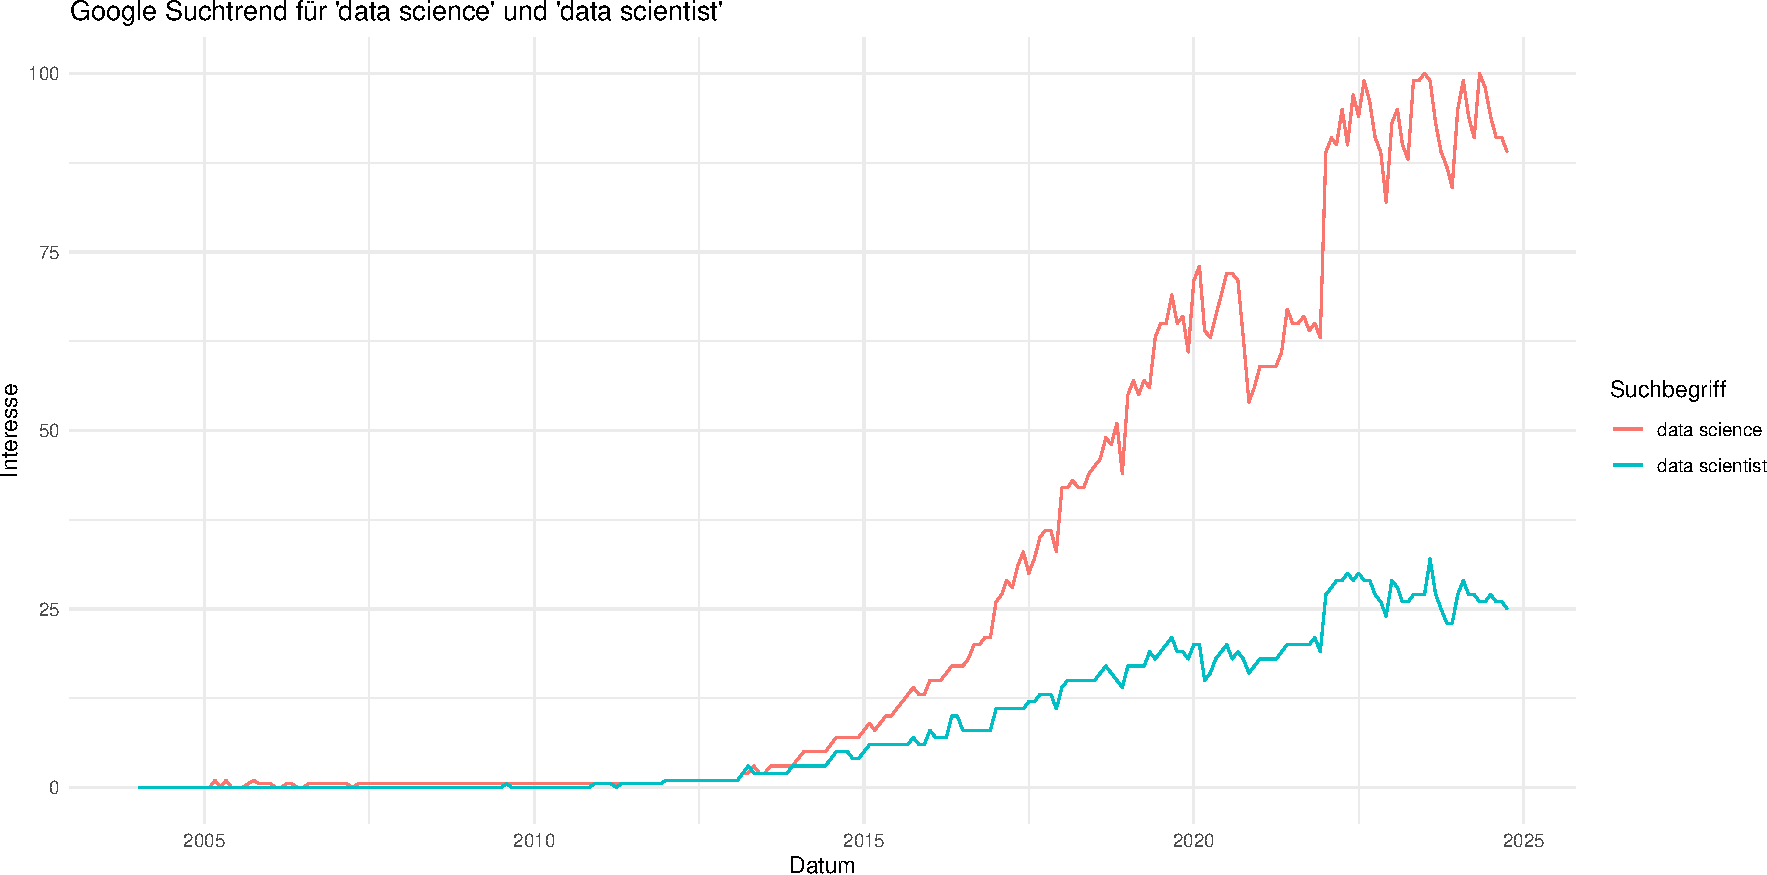
\includegraphics[keepaspectratio]{DataScience_files/figure-latex/unnamed-chunk-2-1.pdf}}
\(\\\) Das wachsende Interesse an Data Science stellt eine große Chance
für Arbeitnehmer dar. Ziel dieser Arbeit ist es einen Überblick über den
Data-Science-Jobmarkt zu geben, um Arbeitnehmern bei der Jobsuche zu
helfen und andererseits einen Überblick über die Gehälter und die Rolle
von Geographie und Wettbewerb bei Jobangeboten und Gehältern zu geben.

\subsection{Forschungsfrage}\label{forschungsfrage}

Im Rahmen der vorliegenden Arbeit wird die folgende Forschungsfrage
bearbeitet:

Es soll untersucht werden, inwiefern die Position und Zentralität von
Unternehmen im Wettbewerbsnetzwerk die Gehaltsstrukturen von
Data-Science-Positionen beeinflusst. Zudem soll erörtert werden, welche
Rolle die Intensität des Wettbewerbs bei der Erklärung von
Gehaltsunterschieden spielt.

Dabei sollen folgende Aspekte untersucht werden:

Bieten Unternehmen, die als zentrale Knoten in einem dichten
Wettbewerbsnetzwerk agieren, tendenziell höhere Löhne an? \(\\\)
Inwieweit beeinflusst die Clusterbildung im Netzwerk die
Gehaltsstrukturen und gibt es spezifische Cluster, in denen höhere
Gehälter häufiger angeboten werden? \(\\\) Welche Zentralitätsmaße
korrelieren signifikant mit überdurchschnittlichen Gehältern und können
Unternehmen mit bestimmten Netzwerkpositionen spezifische
Wettbewerbsvorteile erzielen?

\subsection{Datengrundlage}\label{datengrundlage}

Nachdem die Daten in Python extern als Vorbereitung aufbereitet wurden,
kann nun die Datengrundlage für diese Arbeit in R eingelesen werden.
Dabei wurde sich an
\url{https://www.kaggle.com/code/fahadrehman07/data-science-job-salary-prediction-glassdoor}
orientiert.

\subsubsection{CSV einlesen}\label{csv-einlesen}

\begin{Shaded}
\begin{Highlighting}[]
\NormalTok{data }\OtherTok{\textless{}{-}} \FunctionTok{read\_csv}\NormalTok{(}\StringTok{"data/Glassdoor\_DataScience\_Salary\_modified.csv"}\NormalTok{, }\AttributeTok{show\_col\_types =} \ConstantTok{FALSE}\NormalTok{)}
\end{Highlighting}
\end{Shaded}

Die vorliegende Arbeit basiert auf einem Datensatz von Kaggle, der
Informationen über Data Science Jobs in verschiedenen Unternehmen für
den US-amerikanischen Markt enthält. Der Datensatz umfasst 742 Zeilen
und 28 Spalten, was auf eine Anzahl von 742 verschiedenen Jobangeboten
hindeutet. Diese Anzahl ist kann für die Zwecke dieser Arbeit als
ausreichend zu betrachten, auch wenn eine höhere Zahl an Beobachtungen
möglicherweise zu präziseren Schlussfolgerungen geführt hätte.

Der Datensatz beruht auf Daten, die von Glassdoor extrahiert wurden,
eine für Stellenanzeigen und Unternehmensbewertung bekannte Website, und
bietet detaillierte Informationen über Data-Science-Jobs sowie deren
Gehälter. Der Datensatz beinhaltet wesentliche Informationen, darunter
Jobtitel, geschätzte Gehälter, Stellenbeschreibungen,
Unternehmensbewertungen sowie relevante Unternehmensdaten wie Standort,
Größe und Branche. Eine detaillierte Beschreibung dieser Daten erfolgt
im späteren Verlauf. Der Datensatz eignet sich in besonderem Maße für
den Zweck dieser Arbeit, aber auch für Analysen des Arbeitsmarktes,
beispielsweise zur Untersuchung von Gehaltstrends oder zur
Identifizierung der am besten bewerteten Unternehmen.

Der Datensatz umfasst konkret die folgenden Spalten:

\subsubsection{Erste Ansicht der Daten}\label{erste-ansicht-der-daten}

\begin{Shaded}
\begin{Highlighting}[]
\FunctionTok{head}\NormalTok{(data, }\DecValTok{5}\NormalTok{)}
\end{Highlighting}
\end{Shaded}

\begin{verbatim}
## # A tibble: 5 x 28
##   `Job Title` `Salary Estimate` `Job Description` Rating `Company Name` Location
##   <chr>                   <dbl> <chr>              <dbl> <chr>          <chr>   
## 1 Data Scien~              72   "Data Scientist\~    3.8 Tecolote Rese~ Albuque~
## 2 Healthcare~              87.5 "What You Will D~    3.4 University of~ Linthic~
## 3 Data Scien~              85   "KnowBe4, Inc. i~    4.8 KnowBe4        Clearwa~
## 4 Data Scien~              76.5 "*Organization a~    3.8 PNNL           Richlan~
## 5 Data Scien~             114.  "Data Scientist\~    2.9 Affinity Solu~ New Yor~
## # i 22 more variables: Headquarters <chr>, Size <chr>, Founded <dbl>,
## #   `Type of ownership` <chr>, Industry <chr>, Sector <chr>, Revenue <chr>,
## #   Competitors <chr>, Min_Salary <dbl>, Max_Salary <dbl>, State <chr>,
## #   `Same State` <dbl>, Age <dbl>, Python_yn <dbl>, `R Studio` <dbl>,
## #   Spark <dbl>, AWS_yn <dbl>, Excel_yn <dbl>, Job_simp <chr>, job_state <chr>,
## #   desc_len <dbl>, Num_comp <dbl>
\end{verbatim}

\begin{Shaded}
\begin{Highlighting}[]
\CommentTok{\# Erstellen einer schönen Zusammenfassung des Datensatzes}
\FunctionTok{skim}\NormalTok{(data)}
\end{Highlighting}
\end{Shaded}

\begin{longtable}[]{@{}ll@{}}
\caption{Data summary}\tabularnewline
\toprule\noalign{}
\endfirsthead
\endhead
\bottomrule\noalign{}
\endlastfoot
Name & data \\
Number of rows & 742 \\
Number of columns & 28 \\
\_\_\_\_\_\_\_\_\_\_\_\_\_\_\_\_\_\_\_\_\_\_\_ & \\
Column type frequency: & \\
character & 14 \\
numeric & 14 \\
\_\_\_\_\_\_\_\_\_\_\_\_\_\_\_\_\_\_\_\_\_\_\_\_ & \\
Group variables & None \\
\end{longtable}

\textbf{Variable type: character}

\begin{longtable}[]{@{}
  >{\raggedright\arraybackslash}p{(\linewidth - 14\tabcolsep) * \real{0.2308}}
  >{\raggedleft\arraybackslash}p{(\linewidth - 14\tabcolsep) * \real{0.1282}}
  >{\raggedleft\arraybackslash}p{(\linewidth - 14\tabcolsep) * \real{0.1795}}
  >{\raggedleft\arraybackslash}p{(\linewidth - 14\tabcolsep) * \real{0.0513}}
  >{\raggedleft\arraybackslash}p{(\linewidth - 14\tabcolsep) * \real{0.0769}}
  >{\raggedleft\arraybackslash}p{(\linewidth - 14\tabcolsep) * \real{0.0769}}
  >{\raggedleft\arraybackslash}p{(\linewidth - 14\tabcolsep) * \real{0.1154}}
  >{\raggedleft\arraybackslash}p{(\linewidth - 14\tabcolsep) * \real{0.1410}}@{}}
\toprule\noalign{}
\begin{minipage}[b]{\linewidth}\raggedright
skim\_variable
\end{minipage} & \begin{minipage}[b]{\linewidth}\raggedleft
n\_missing
\end{minipage} & \begin{minipage}[b]{\linewidth}\raggedleft
complete\_rate
\end{minipage} & \begin{minipage}[b]{\linewidth}\raggedleft
min
\end{minipage} & \begin{minipage}[b]{\linewidth}\raggedleft
max
\end{minipage} & \begin{minipage}[b]{\linewidth}\raggedleft
empty
\end{minipage} & \begin{minipage}[b]{\linewidth}\raggedleft
n\_unique
\end{minipage} & \begin{minipage}[b]{\linewidth}\raggedleft
whitespace
\end{minipage} \\
\midrule\noalign{}
\endhead
\bottomrule\noalign{}
\endlastfoot
Job Title & 0 & 1 & 9 & 98 & 0 & 264 & 0 \\
Job Description & 0 & 1 & 407 & 10051 & 0 & 463 & 0 \\
Company Name & 0 & 1 & 2 & 51 & 0 & 343 & 0 \\
Location & 0 & 1 & 8 & 33 & 0 & 200 & 0 \\
Headquarters & 0 & 1 & 2 & 26 & 0 & 198 & 0 \\
Size & 0 & 1 & 2 & 23 & 0 & 9 & 0 \\
Type of ownership & 0 & 1 & 2 & 30 & 0 & 11 & 0 \\
Industry & 0 & 1 & 2 & 40 & 0 & 60 & 0 \\
Sector & 0 & 1 & 2 & 34 & 0 & 25 & 0 \\
Revenue & 0 & 1 & 2 & 32 & 0 & 14 & 0 \\
Competitors & 0 & 1 & 2 & 92 & 0 & 128 & 0 \\
State & 0 & 1 & 2 & 11 & 0 & 38 & 0 \\
Job\_simp & 0 & 1 & 2 & 14 & 0 & 7 & 0 \\
job\_state & 0 & 1 & 2 & 2 & 0 & 37 & 0 \\
\end{longtable}

\textbf{Variable type: numeric}

\begin{longtable}[]{@{}
  >{\raggedright\arraybackslash}p{(\linewidth - 20\tabcolsep) * \real{0.1684}}
  >{\raggedleft\arraybackslash}p{(\linewidth - 20\tabcolsep) * \real{0.1053}}
  >{\raggedleft\arraybackslash}p{(\linewidth - 20\tabcolsep) * \real{0.1474}}
  >{\raggedleft\arraybackslash}p{(\linewidth - 20\tabcolsep) * \real{0.0842}}
  >{\raggedleft\arraybackslash}p{(\linewidth - 20\tabcolsep) * \real{0.0842}}
  >{\raggedleft\arraybackslash}p{(\linewidth - 20\tabcolsep) * \real{0.0632}}
  >{\raggedleft\arraybackslash}p{(\linewidth - 20\tabcolsep) * \real{0.0737}}
  >{\raggedleft\arraybackslash}p{(\linewidth - 20\tabcolsep) * \real{0.0737}}
  >{\raggedleft\arraybackslash}p{(\linewidth - 20\tabcolsep) * \real{0.0737}}
  >{\raggedleft\arraybackslash}p{(\linewidth - 20\tabcolsep) * \real{0.0632}}
  >{\raggedright\arraybackslash}p{(\linewidth - 20\tabcolsep) * \real{0.0632}}@{}}
\toprule\noalign{}
\begin{minipage}[b]{\linewidth}\raggedright
skim\_variable
\end{minipage} & \begin{minipage}[b]{\linewidth}\raggedleft
n\_missing
\end{minipage} & \begin{minipage}[b]{\linewidth}\raggedleft
complete\_rate
\end{minipage} & \begin{minipage}[b]{\linewidth}\raggedleft
mean
\end{minipage} & \begin{minipage}[b]{\linewidth}\raggedleft
sd
\end{minipage} & \begin{minipage}[b]{\linewidth}\raggedleft
p0
\end{minipage} & \begin{minipage}[b]{\linewidth}\raggedleft
p25
\end{minipage} & \begin{minipage}[b]{\linewidth}\raggedleft
p50
\end{minipage} & \begin{minipage}[b]{\linewidth}\raggedleft
p75
\end{minipage} & \begin{minipage}[b]{\linewidth}\raggedleft
p100
\end{minipage} & \begin{minipage}[b]{\linewidth}\raggedright
hist
\end{minipage} \\
\midrule\noalign{}
\endhead
\bottomrule\noalign{}
\endlastfoot
Salary Estimate & 0 & 1 & 100.63 & 38.86 & 13.5 & 73.5 & 97.5 & 122.5 &
254 & ▂▇▅▁▁ \\
Rating & 0 & 1 & 3.62 & 0.80 & -1.0 & 3.3 & 3.7 & 4.0 & 5 & ▁▁▁▇▅ \\
Founded & 0 & 1 & 1837.15 & 497.18 & -1.0 & 1939.0 & 1988.0 & 2007.0 &
2019 & ▁▁▁▁▇ \\
Min\_Salary & 0 & 1 & 74.72 & 30.98 & 15.0 & 52.0 & 69.5 & 91.0 & 202 &
▅▇▃▁▁ \\
Max\_Salary & 0 & 1 & 127.18 & 46.91 & 16.0 & 96.0 & 124.0 & 155.0 & 306
& ▂▇▆▂▁ \\
Same State & 0 & 1 & 0.56 & 0.50 & 0.0 & 0.0 & 1.0 & 1.0 & 1 & ▆▁▁▁▇ \\
Age & 0 & 1 & 49.39 & 53.96 & -1.0 & 14.0 & 27.0 & 62.0 & 279 & ▇▂▁▁▁ \\
Python\_yn & 0 & 1 & 0.53 & 0.50 & 0.0 & 0.0 & 1.0 & 1.0 & 1 & ▇▁▁▁▇ \\
R Studio & 0 & 1 & 0.00 & 0.05 & 0.0 & 0.0 & 0.0 & 0.0 & 1 & ▇▁▁▁▁ \\
Spark & 0 & 1 & 0.23 & 0.42 & 0.0 & 0.0 & 0.0 & 0.0 & 1 & ▇▁▁▁▂ \\
AWS\_yn & 0 & 1 & 0.24 & 0.43 & 0.0 & 0.0 & 0.0 & 0.0 & 1 & ▇▁▁▁▂ \\
Excel\_yn & 0 & 1 & 0.52 & 0.50 & 0.0 & 0.0 & 1.0 & 1.0 & 1 & ▇▁▁▁▇ \\
desc\_len & 0 & 1 & 3869.55 & 1521.50 & 407.0 & 2801.0 & 3731.0 & 4740.0
& 10051 & ▂▇▅▁▁ \\
Num\_comp & 0 & 1 & 1.05 & 1.38 & 0.0 & 0.0 & 0.0 & 3.0 & 4 & ▇▁▁▃▁ \\
\end{longtable}

Im Folgenden wird eine Übersicht der wesentlichen Spalten präsentiert:

\begin{itemize}
\tightlist
\item
  \texttt{Job\ Title}: Die Berufsbezeichnung, sie gibt Aufschluss über
  die Tätigkeit.
\item
  \texttt{Salary\ Estimate}: Die geschätzte Gehalt, in tausend Dollar
  pro Jahr. Es basiert auf dem Durchschnitt von dem minimalen und
  maximalen Gehalt.
\item
  \texttt{Job\ Description}, \texttt{Job\_simp}: Die Beschreibung der
  Stelle, die Aufgaben und Anforderungen enthält. Auch die vereinfachte
  Version der Berufsbezeichnung.
\item
  \texttt{Rating}: Die Bewertung des Unternehmens, sie weist eine
  Spannbreite von 1 bis 5 auf, wobei die Bewertung ``-1'' bei jeder
  Spalte für fehlende Bewertungen steht.
\item
  \texttt{Company\ Name}, \texttt{Location}, \texttt{Headquarters},
  \texttt{Size}, \texttt{Founded}: Unternehmensbezogene Daten wie Name,
  Standort, Sitz, Größe und Gründungsjahr des Unternehmens.
\item
  \texttt{Type\ of\ ownership}, \texttt{Industry}, \texttt{Sector},
  \texttt{Revenue}: Weitere Unternehmensmerkmale, diese umfassen die
  Eigentumsart, die Branche, den Sektor sowie die Einnahmen.
\item
  \texttt{Competitors}: Die Wettbewerber des Unternehmens, die im
  Zusammenhang dieser Arbeit von besonderer Bedeutung sind.
\item
  Skills (\texttt{Python\_yn}, \texttt{R\ Studio}, \texttt{Spark},
  \texttt{AWS\_yn}, \texttt{Excel\_yn}): Spalten, aus denen hervorgeht,
  ob die betreffende Kompetenz in der Stellenbeschreibung verlangt wird
  (0 = nein, 1 = ja).
\item
  \texttt{Min\_salary}, \texttt{Max\_salary}: Minimale und maximale
  Gehaltsschätzungen.
\item
  \texttt{State}, \texttt{Same\ State}, \texttt{job\_state},
  \texttt{Age}, \texttt{desc\_len}, \texttt{Num\_comp}: Zusätzliche
  Informationen wie Standort der Stelle, Alter des Unternehmens, Länge
  der Stellenbeschreibung und Anzahl der Mitbewerber.
\end{itemize}

Es zeigt sich, dass eine Vielzahl von Spalten für die vorliegende
Untersuchung irrelevant ist. Infolgedessen werden in einem späteren Teil
der Arbeit irrelevante Spalten, wie beispielsweise die Kenntnisse in
Python, R Studio, Spark und ähnlichen Programmen, welche ursprünglich
aus der Jobbeschreibung extrahiert wurden, entfernt.

Im Folgenden wird eine erste Betrachtung der Daten vorgenommen. Zu
diesem Zweck werden die Jobs in New York nach ihren jeweiligen
Vergütungen geordnet und in Form eines Balkendiagramms dargestellt.

\begin{Shaded}
\begin{Highlighting}[]
\CommentTok{\# Filterung der Daten für New York}
\NormalTok{data\_ny }\OtherTok{\textless{}{-}}\NormalTok{ data }\SpecialCharTok{\%\textgreater{}\%}
  \FunctionTok{filter}\NormalTok{(State }\SpecialCharTok{==} \StringTok{"NY"}\NormalTok{)}

\CommentTok{\# Durchschnittsgehalt nach Berufsbezeichnung}
\NormalTok{avg\_salary\_by\_job\_ny }\OtherTok{\textless{}{-}}\NormalTok{ data\_ny }\SpecialCharTok{\%\textgreater{}\%}
  \FunctionTok{group\_by}\NormalTok{(}\StringTok{\textasciigrave{}}\AttributeTok{Job Title}\StringTok{\textasciigrave{}}\NormalTok{) }\SpecialCharTok{\%\textgreater{}\%}
  \FunctionTok{summarise}\NormalTok{(}\AttributeTok{Average\_Salary =} \FunctionTok{mean}\NormalTok{(}\StringTok{\textasciigrave{}}\AttributeTok{Salary Estimate}\StringTok{\textasciigrave{}}\NormalTok{, }\AttributeTok{na.rm =} \ConstantTok{TRUE}\NormalTok{)) }\SpecialCharTok{\%\textgreater{}\%}
  \FunctionTok{arrange}\NormalTok{(}\FunctionTok{desc}\NormalTok{(Average\_Salary))}

\CommentTok{\# Bar Plot}
\FunctionTok{ggplot}\NormalTok{(avg\_salary\_by\_job\_ny,}
       \FunctionTok{aes}\NormalTok{(}\AttributeTok{x =} \FunctionTok{reorder}\NormalTok{(}\StringTok{\textasciigrave{}}\AttributeTok{Job Title}\StringTok{\textasciigrave{}}\NormalTok{, Average\_Salary), }\AttributeTok{y =}\NormalTok{ Average\_Salary)) }\SpecialCharTok{+}
  \FunctionTok{geom\_bar}\NormalTok{(}\AttributeTok{stat =} \StringTok{"identity"}\NormalTok{) }\SpecialCharTok{+}
  \FunctionTok{coord\_flip}\NormalTok{() }\SpecialCharTok{+}
  \FunctionTok{labs}\NormalTok{(}\AttributeTok{title =} \StringTok{"Average Salary by Job Title in NY"}\NormalTok{,}
       \AttributeTok{x =} \StringTok{"Job Title"}\NormalTok{,}
       \AttributeTok{y =} \StringTok{"Average Salary"}\NormalTok{) }\SpecialCharTok{+}
  \FunctionTok{theme\_minimal}\NormalTok{() }\SpecialCharTok{+}
  \FunctionTok{theme}\NormalTok{(}
    \AttributeTok{axis.title =} \FunctionTok{element\_text}\NormalTok{(}\AttributeTok{size =} \DecValTok{14}\NormalTok{),}
    \AttributeTok{axis.text =} \FunctionTok{element\_text}\NormalTok{(}\AttributeTok{size =} \DecValTok{12}\NormalTok{),}
    \AttributeTok{plot.title =} \FunctionTok{element\_text}\NormalTok{(}\AttributeTok{size =} \DecValTok{16}\NormalTok{, }\AttributeTok{face =} \StringTok{"bold"}\NormalTok{)}
\NormalTok{  )}
\end{Highlighting}
\end{Shaded}

\pandocbounded{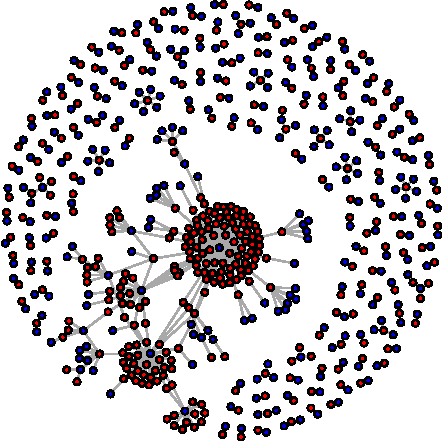
\includegraphics[keepaspectratio]{DataScience_files/figure-latex/unnamed-chunk-5-1.pdf}}
Es lässt sich eine signifikante Variation der Gehälter in New York
beobachten. Zudem zeigt sich eine Korrelation zwischen Höhe des Gehalts
und der Position: Mit steigendem Einkommen nehmen die Anzahl und der
Rang der Senior- und Managerpositionen zu.

\begin{center}\rule{0.5\linewidth}{0.5pt}\end{center}

Da die Datengrundlage nicht in einem igraph-Objekt vorliegt und
ungerichtet ist, ist es notwendig Knoten, Kanten sowie relevante
Attribute wie beispielsweise Gewichtungen zu definieren, um überhaupt
Netzwerkvisualisierungen in R durchführen zu können. Doch dazu mehr im
nächsten Kapitel.

\newpage

\section{Analysestrategie}\label{analysestrategie}

Im Rahmen meiner Analyse werde ich die verschiedenen Zentralitätsmaße
zur Untersuchung der Position und Bedeutung von Unternehmen im
Wettbewerbsnetzwerk heranziehen. Die Anwendung dieser Maße ermöglicht
unterschiedlicher Einblicke in die strategische Verknüpfung von
Unternehmen im Netzwerk sowie in die potenzielle Auswirkung dieser
Verknüpfung auf die Gehaltspolitik und Attraktivität von Unternehmen im
Data-Science-Bereich.

\textbf{1. Datenaufbereitung und Netzwerkerstellung}

In einem ersten Schritt wird ein Netzwerk aufgebaut, in dem jedes
Unternehmen als Knoten dargestellt wird. Die Verbindungen zwischen den
Knoten basieren auf der Spalte ``Competitors''. Dabei werden
Unternehmen, die als Wettbewerber aufgeführt sind, durch eine Kante
verbunden. Im nächsten Schritt erfolgt eine Aufbereitung der Daten. Dazu
werden doppelte oder fehlerhafte Einträge entfernt sowie
Unternehmensnamen standardisiert, um eine korrekte Kantenbildung zu
gewährleisten.

\textbf{2. Berechnung von Netzwerkmetriken und Zentralitätsmaßen}

In der nächsten Phase erfolgt die Berechnung wichtiger
Zentralitätsmetriken, welche die Bedeutung der einzelnen Unternehmen im
Wettbewerbsnetzwerk bestimmen. Die Betweenness-Zentralität ermöglicht
die Identifikation von Unternehmen, die eine Brückenfunktion zwischen
anderen Unternehmen einnehmen. Diese Unternehmen sind von entscheidender
Bedeutung für die Kommunikation und den Austausch von Informationen
innerhalb des Netzwerkes. Die Degree-Zentralität gibt Aufschluss über
die Anzahl direkter Wettbewerber, mit denen ein Unternehmen in Beziehung
steht. Dies reflektiert die Wettbewerbsintensität und gibt Aufschluss
über die Integration eines Unternehmens in das Wettbewerbsumfeld. Die
Eigenvektor-Zentralität demonstriert die besondere Einflussnahme von
Unternehmen, welche durch eine exzellente Vernetzung mit anderen
zentralen Wettbewerbern gekennzeichnet ist.

\textbf{3. Visualisierung und Strukturanalyse des Wettbewerbsnetzwerks}

Im Folgenden erfolgt eine Anwendung von Algorithmen zur Erkennung von
Communities, wie beispielsweise Louvain, mit dem Ziel, Cluster innerhalb
des Netzwerks zu identifizieren. Die Analyse zielt darauf ab, natürliche
Gruppen von Unternehmen zu identifizieren, die durch intensive
Wettbewerbsverhältnisse gekennzeichnet sind. Des Weiteren erfolgt
innerhalb der identifizierten Cluster eine Analyse der Gehaltsstrukturen
sowie der Branchenzugehörigkeit, mit dem Ziel, etwaige Muster und
Zusammenhänge zu identifizieren.

\textbf{4. Explorative Gehaltsanalyse im Netzwerk}

Abschließen wird im Rahmen einer explorativen Gehaltsanalyse dem Leser
die Möglichkeit gegeben die Gehaltsstrukturen innerhalb des Netzwerkes
gemeinsam mit den Zentralitätsmaßen selbstständig zu erforschen.

\newpage

\section{Analyse}\label{analyse}

\subsection{Datenbereinigung}\label{datenbereinigung}

\subsubsection{Bereinigung für die geografische
Analysex}\label{bereinigung-fuxfcr-die-geografische-analysex}

Bei der Durchsicht des Datensatzes viel auf, dass die Spalten ``Same
State'' und ``job\_state'' von der Logik her ähnlich sind. Dies soll nun
näher unterucht werden, um spätere Fehler, vor allem bei geografischen
Netzwerken(siehe Anhang), vorzubeugen. \(\\\)

\begin{Shaded}
\begin{Highlighting}[]
\CommentTok{\# Auswahl der "State" und "job\_state" Spalten}
\NormalTok{selected\_data }\OtherTok{\textless{}{-}}\NormalTok{ data }\SpecialCharTok{\%\textgreater{}\%}
  \FunctionTok{select}\NormalTok{(State, job\_state)}

\CommentTok{\# Heading der ausgewählten Spalten}
\FunctionTok{head}\NormalTok{(selected\_data, }\DecValTok{15}\NormalTok{)}
\end{Highlighting}
\end{Shaded}

\begin{verbatim}
## # A tibble: 15 x 2
##    State job_state
##    <chr> <chr>    
##  1 NM    NM       
##  2 MD    MD       
##  3 FL    FL       
##  4 WA    WA       
##  5 NY    NY       
##  6 TX    TX       
##  7 MD    MD       
##  8 CA    CA       
##  9 NY    NY       
## 10 NY    NY       
## 11 CA    CA       
## 12 VA    VA       
## 13 TX    TX       
## 14 WA    WA       
## 15 MA    MA
\end{verbatim}

Es scheint, dass beide Spalten identisch sind. Diesbezüglich ist jedoch
eine Prüfung erforderlich. \(\\\)

\begin{Shaded}
\begin{Highlighting}[]
\ControlFlowTok{if}\NormalTok{ (}\FunctionTok{all}\NormalTok{(selected\_data}\SpecialCharTok{$}\NormalTok{State }\SpecialCharTok{==}\NormalTok{ selected\_data}\SpecialCharTok{$}\NormalTok{job\_state, }\AttributeTok{na.rm =} \ConstantTok{TRUE}\NormalTok{)) \{}
  \FunctionTok{print}\NormalTok{(}\StringTok{"Alle Werte in \textquotesingle{}State\textquotesingle{} und \textquotesingle{}job\_state\textquotesingle{} sind identisch."}\NormalTok{)}
\NormalTok{\} }\ControlFlowTok{else}\NormalTok{ \{}
  \FunctionTok{print}\NormalTok{(}\StringTok{"Es gibt Unterschiede zwischen \textquotesingle{}State\textquotesingle{} und \textquotesingle{}job\_state\textquotesingle{}."}\NormalTok{)}
\NormalTok{\}}
\end{Highlighting}
\end{Shaded}

\begin{verbatim}
## [1] "Es gibt Unterschiede zwischen 'State' und 'job_state'."
\end{verbatim}

Diese Annahme erweist sich jedoch als unzutreffend, da sich in der Tat
Unterschiede feststellen lassen. \(\\\)

\begin{Shaded}
\begin{Highlighting}[]
\CommentTok{\# Auswahl der Zeilen, in denen "State" und "job\_state" unterschiedlich sind}
\NormalTok{different\_states }\OtherTok{\textless{}{-}}\NormalTok{ selected\_data }\SpecialCharTok{\%\textgreater{}\%}
  \FunctionTok{filter}\NormalTok{(State }\SpecialCharTok{!=}\NormalTok{ job\_state)}

\FunctionTok{print}\NormalTok{(different\_states, }\AttributeTok{n =} \ConstantTok{Inf}\NormalTok{)}
\end{Highlighting}
\end{Shaded}

\begin{verbatim}
## # A tibble: 1 x 2
##   State       job_state
##   <chr>       <chr>    
## 1 Los Angeles CA
\end{verbatim}

Es fällt auf, dass LA und Los Angeles nicht einheitlich verwendet
werden. Außerdem ist Los Angeles kein eigener Bundesstaat, sondern ein
Teil von Kalifornien (CA). Dies sollte korrigiert werden. \(\\\)
Außerdem sollte bei der weiteren Vorgehensweise darauf geachtet werden,
dass Werte wie ``Na'' oder ``-1'' vor den Auswertungen entfernt werden.
\(\\\)

\begin{Shaded}
\begin{Highlighting}[]
\CommentTok{\# Ersetzen von "Los Angeles" durch "LA" und "LA" durch "CA"}
\NormalTok{data }\OtherTok{\textless{}{-}}\NormalTok{ data }\SpecialCharTok{\%\textgreater{}\%}
  \FunctionTok{mutate}\NormalTok{(}\AttributeTok{State =} \FunctionTok{ifelse}\NormalTok{(State }\SpecialCharTok{==} \StringTok{"Los Angeles"}\NormalTok{, }\StringTok{"LA"}\NormalTok{, State),}
         \AttributeTok{job\_state =} \FunctionTok{ifelse}\NormalTok{(job\_state }\SpecialCharTok{==} \StringTok{"Los Angeles"}\NormalTok{, }\StringTok{"LA"}\NormalTok{, job\_state))}

\NormalTok{data }\OtherTok{\textless{}{-}}\NormalTok{ data }\SpecialCharTok{\%\textgreater{}\%}
  \FunctionTok{mutate}\NormalTok{(}\AttributeTok{State =} \FunctionTok{ifelse}\NormalTok{(State }\SpecialCharTok{==} \StringTok{"LA"}\NormalTok{, }\StringTok{"CA"}\NormalTok{, State),}
         \AttributeTok{job\_state =} \FunctionTok{ifelse}\NormalTok{(job\_state }\SpecialCharTok{==} \StringTok{"LA"}\NormalTok{, }\StringTok{"CA"}\NormalTok{, job\_state))}

\CommentTok{\# Erneute Überprüfung}
\NormalTok{selected\_data }\OtherTok{\textless{}{-}}\NormalTok{ data }\SpecialCharTok{\%\textgreater{}\%}
  \FunctionTok{select}\NormalTok{(State, job\_state)}

\ControlFlowTok{if}\NormalTok{ (}\FunctionTok{all}\NormalTok{(selected\_data}\SpecialCharTok{$}\NormalTok{State }\SpecialCharTok{==}\NormalTok{ selected\_data}\SpecialCharTok{$}\NormalTok{job\_state, }\AttributeTok{na.rm =} \ConstantTok{TRUE}\NormalTok{)) \{}
  \FunctionTok{print}\NormalTok{(}\StringTok{"Alle Werte in \textquotesingle{}State\textquotesingle{} und \textquotesingle{}job\_state\textquotesingle{} sind identisch."}\NormalTok{)}
\NormalTok{\} }\ControlFlowTok{else}\NormalTok{ \{}
  \FunctionTok{print}\NormalTok{(}\StringTok{"Es gibt Unterschiede zwischen \textquotesingle{}State\textquotesingle{} und \textquotesingle{}job\_state\textquotesingle{}."}\NormalTok{)}
\NormalTok{\}}
\end{Highlighting}
\end{Shaded}

\begin{verbatim}
## [1] "Alle Werte in 'State' und 'job_state' sind identisch."
\end{verbatim}

\subsubsection{Überprüfung auf weitere fehlende
Werte}\label{uxfcberpruxfcfung-auf-weitere-fehlende-werte}

Im nächsten Schritt wird der Datensatz auf weitere fehlende Werte
überprüft, um sicherzustellen, dass keine fehlerhaften Daten in die
Analyse einfließen. \(\\\)

\begin{Shaded}
\begin{Highlighting}[]
\CommentTok{\# Überprüfen auf NA{-}Werte}
\NormalTok{na\_counts }\OtherTok{\textless{}{-}} \FunctionTok{colSums}\NormalTok{(}\FunctionTok{is.na}\NormalTok{(data))}

\CommentTok{\# Anzahl der NA{-}Werte pro Spalte:}
\FunctionTok{print}\NormalTok{(na\_counts)}
\end{Highlighting}
\end{Shaded}

\begin{verbatim}
##         Job Title   Salary Estimate   Job Description            Rating 
##                 0                 0                 0                 0 
##      Company Name          Location      Headquarters              Size 
##                 0                 0                 0                 0 
##           Founded Type of ownership          Industry            Sector 
##                 0                 0                 0                 0 
##           Revenue       Competitors        Min_Salary        Max_Salary 
##                 0                 0                 0                 0 
##             State        Same State               Age         Python_yn 
##                 0                 0                 0                 0 
##          R Studio             Spark            AWS_yn          Excel_yn 
##                 0                 0                 0                 0 
##          Job_simp         job_state          desc_len          Num_comp 
##                 0                 0                 0                 0
\end{verbatim}

\begin{Shaded}
\begin{Highlighting}[]
\CommentTok{\# Überprüfen auf "na"{-}Werte (kleingeschrieben)}
\NormalTok{na\_string\_counts }\OtherTok{\textless{}{-}} \FunctionTok{sapply}\NormalTok{(data, }\ControlFlowTok{function}\NormalTok{(x) }\FunctionTok{sum}\NormalTok{(}\FunctionTok{tolower}\NormalTok{(x) }\SpecialCharTok{==} \StringTok{"na"}\NormalTok{, }\AttributeTok{na.rm =} \ConstantTok{TRUE}\NormalTok{))}

\CommentTok{\# Anzahl der "na"{-}Werte pro Spalte:}
\FunctionTok{print}\NormalTok{(na\_string\_counts)}
\end{Highlighting}
\end{Shaded}

\begin{verbatim}
##         Job Title   Salary Estimate   Job Description            Rating 
##                 0                 0                 0                 0 
##      Company Name          Location      Headquarters              Size 
##                 0                 0                 0                 0 
##           Founded Type of ownership          Industry            Sector 
##                 0                 0                 0                 0 
##           Revenue       Competitors        Min_Salary        Max_Salary 
##                 0                 0                 0                 0 
##             State        Same State               Age         Python_yn 
##                 0                 0                 0                 0 
##          R Studio             Spark            AWS_yn          Excel_yn 
##                 0                 0                 0                 0 
##          Job_simp         job_state          desc_len          Num_comp 
##               184                 0                 0                 0
\end{verbatim}

\begin{Shaded}
\begin{Highlighting}[]
\CommentTok{\# Überprüfen auf {-}1{-}Werte}
\NormalTok{neg\_one\_counts }\OtherTok{\textless{}{-}} \FunctionTok{sapply}\NormalTok{(data, }\ControlFlowTok{function}\NormalTok{(x) }\FunctionTok{sum}\NormalTok{(x }\SpecialCharTok{==} \SpecialCharTok{{-}}\DecValTok{1}\NormalTok{, }\AttributeTok{na.rm =} \ConstantTok{TRUE}\NormalTok{))}

\CommentTok{\# Anzahl der {-}1 Werte in der Spalte Competitors}
\FunctionTok{print}\NormalTok{(neg\_one\_counts)}
\end{Highlighting}
\end{Shaded}

\begin{verbatim}
##         Job Title   Salary Estimate   Job Description            Rating 
##                 0                 0                 0                11 
##      Company Name          Location      Headquarters              Size 
##                 0                 0                 1                 1 
##           Founded Type of ownership          Industry            Sector 
##                50                 1                10                10 
##           Revenue       Competitors        Min_Salary        Max_Salary 
##                 1               460                 0                 0 
##             State        Same State               Age         Python_yn 
##                 0                 0                50                 0 
##          R Studio             Spark            AWS_yn          Excel_yn 
##                 0                 0                 0                 0 
##          Job_simp         job_state          desc_len          Num_comp 
##                 0                 0                 0                 0
\end{verbatim}

\(\\\) Es zeigt sich, dass lediglich in der Spalte ``Competitors''
relevante negative Werte zu finden sind, welche nun entfernt werden
müssen. Die ``na''-Werte in der Spalte ``Job\_simp'' hingegen haben
keinen Einfluss auf die Analyse. \(\\\)

\begin{Shaded}
\begin{Highlighting}[]
\CommentTok{\# Entfernen von Zeilen mit {-}1 Werten in der Spalte "Competitors"}
\NormalTok{data }\OtherTok{\textless{}{-}}\NormalTok{ data }\SpecialCharTok{\%\textgreater{}\%}
  \FunctionTok{filter}\NormalTok{(Competitors }\SpecialCharTok{!=} \SpecialCharTok{{-}}\DecValTok{1}\NormalTok{)}

\CommentTok{\# Überprüfen auf {-}1{-}Werte nach Entfernung}
\NormalTok{neg\_one\_counts }\OtherTok{\textless{}{-}} \FunctionTok{sapply}\NormalTok{(data, }\ControlFlowTok{function}\NormalTok{(x) }\FunctionTok{sum}\NormalTok{(x }\SpecialCharTok{==} \SpecialCharTok{{-}}\DecValTok{1}\NormalTok{, }\AttributeTok{na.rm =} \ConstantTok{TRUE}\NormalTok{))}
\CommentTok{\# Anzahl der {-}1 Werte pro Spalte:}
\FunctionTok{print}\NormalTok{(neg\_one\_counts)}
\end{Highlighting}
\end{Shaded}

\begin{verbatim}
##         Job Title   Salary Estimate   Job Description            Rating 
##                 0                 0                 0                 0 
##      Company Name          Location      Headquarters              Size 
##                 0                 0                 0                 0 
##           Founded Type of ownership          Industry            Sector 
##                 1                 0                 0                 0 
##           Revenue       Competitors        Min_Salary        Max_Salary 
##                 0                 0                 0                 0 
##             State        Same State               Age         Python_yn 
##                 0                 0                 1                 0 
##          R Studio             Spark            AWS_yn          Excel_yn 
##                 0                 0                 0                 0 
##          Job_simp         job_state          desc_len          Num_comp 
##                 0                 0                 0                 0
\end{verbatim}

\subsubsection{Entfernen irrelevanter
Spalten}\label{entfernen-irrelevanter-spalten}

In einem nächsten Schritt werden auf Basis der zuvor festgelegten
Analysestrategie sowie der geplanten Analysen diejenigen Spalten
identifiziert, die für die Analysen nicht erforderlich sind und
anschließend entfernt. \(\\\)

\begin{Shaded}
\begin{Highlighting}[]
\CommentTok{\# Entfernen irrelevanter Spalten}
\NormalTok{data }\OtherTok{\textless{}{-}}\NormalTok{ data }\SpecialCharTok{\%\textgreater{}\%}
  \FunctionTok{select}\NormalTok{(}\SpecialCharTok{{-}}\FunctionTok{c}\NormalTok{(}\StringTok{\textasciigrave{}}\AttributeTok{Job Description}\StringTok{\textasciigrave{}}\NormalTok{, Rating, Headquarters, Size, Founded,}
            \StringTok{\textasciigrave{}}\AttributeTok{Type of ownership}\StringTok{\textasciigrave{}}\NormalTok{, Sector, Revenue, Python\_yn,}
            \StringTok{\textasciigrave{}}\AttributeTok{R Studio}\StringTok{\textasciigrave{}}\NormalTok{, Spark, AWS\_yn, Excel\_yn, desc\_len, Num\_comp))}

\CommentTok{\# Ausgeben der noch enthaltenen Spalten}
\FunctionTok{print}\NormalTok{(data }\SpecialCharTok{\%\textgreater{}\%} \FunctionTok{names}\NormalTok{())}
\end{Highlighting}
\end{Shaded}

\begin{verbatim}
##  [1] "Job Title"       "Salary Estimate" "Company Name"    "Location"       
##  [5] "Industry"        "Competitors"     "Min_Salary"      "Max_Salary"     
##  [9] "State"           "Same State"      "Age"             "Job_simp"       
## [13] "job_state"
\end{verbatim}

\subsubsection{Bereinigung irrelevanter
Jobtitel}\label{bereinigung-irrelevanter-jobtitel}

Im Rahmen dieser Arbeit erfolgt eine Analyse von Gehältern und
Wettbewerbsbeziehungen für den Data-Science-Jobmarkt. Dabei ist zu
überprüfen, ob alle Spalten tatsächlich konkrete Data-Science-Jobs
repräsentieren.

Bei einer ersten Betrachtung des in der Einleitung präsentierten
Balkendiagramms wird ersichtlich, dass eine Reihe von Jobtiteln nicht
unmittelbar mit dem Bereich der ``Data Science'' assoziiert werden
können. \(\\\)

\begin{Shaded}
\begin{Highlighting}[]
\CommentTok{\# ausgeben alles uniqeuen Job Title und Job\_simp}
\FunctionTok{print}\NormalTok{(data }\SpecialCharTok{\%\textgreater{}\%} \FunctionTok{select}\NormalTok{(}\StringTok{\textasciigrave{}}\AttributeTok{Job Title}\StringTok{\textasciigrave{}}\NormalTok{, }\StringTok{\textasciigrave{}}\AttributeTok{Job\_simp}\StringTok{\textasciigrave{}}\NormalTok{) }\SpecialCharTok{\%\textgreater{}\%} \FunctionTok{unique}\NormalTok{())}
\end{Highlighting}
\end{Shaded}

\begin{verbatim}
## # A tibble: 111 x 2
##    `Job Title`                                                     Job_simp     
##    <chr>                                                           <chr>        
##  1 Data Scientist                                                  data scienti~
##  2 Staff Data Scientist - Technology                               data scienti~
##  3 Scientist I/II, Biology                                         na           
##  4 Data Analyst                                                    analyst      
##  5 Scientist                                                       na           
##  6 Senior Data Scientist                                           data scienti~
##  7 Lead Data Scientist                                             data scienti~
##  8 Spectral Scientist/Engineer                                     na           
##  9 College Hire - Data Scientist - Open to December 2019 Graduates data scienti~
## 10 Data Scientist, Office of Data Science                          data scienti~
## # i 101 more rows
\end{verbatim}

Es lässt sich feststellen, dass der Datensatz auch eine Reihe von Jobs
von Wissenschaftlern umfasst, die nicht unmittelbar mit Data Science
assoziiert werden. Diese Jobs sind zudem nicht mit einem vereinfachten
Jobtitel (``Job\_simp'') versehen, der auf eine Tätigkeit im Bereich
Data Science hinweist. Daher ist es erforderlich, alle Datensätze mit
na-Werten in der Spalte ``Job\_simp'' zu eliminieren. Diese besutzen
auch eine andere Schreibweise, deswegen wurden sie nicht direkt
entfernt. \(\\\)

\begin{Shaded}
\begin{Highlighting}[]
\CommentTok{\# Entfernen von Zeilen mit NA{-}Werten in der Spalte "Job\_simp"}
\NormalTok{data }\OtherTok{\textless{}{-}}\NormalTok{ data }\SpecialCharTok{\%\textgreater{}\%}
  \FunctionTok{filter}\NormalTok{(Job\_simp }\SpecialCharTok{!=} \StringTok{"na"}\NormalTok{)}

\CommentTok{\# Überprüfen auf "na"{-}Werte in der Spalte "Job\_simp"}
\NormalTok{na\_job\_simp }\OtherTok{\textless{}{-}} \FunctionTok{sum}\NormalTok{(data}\SpecialCharTok{$}\NormalTok{Job\_simp }\SpecialCharTok{==} \StringTok{"na"}\NormalTok{)}

\FunctionTok{print}\NormalTok{(}\FunctionTok{paste}\NormalTok{(}\StringTok{"Anzahl der \textquotesingle{}na\textquotesingle{}{-}Werte in der Spalte \textquotesingle{}Job\_simp\textquotesingle{}:"}\NormalTok{, na\_job\_simp))}
\end{Highlighting}
\end{Shaded}

\begin{verbatim}
## [1] "Anzahl der 'na'-Werte in der Spalte 'Job_simp': 0"
\end{verbatim}

\begin{Shaded}
\begin{Highlighting}[]
\FunctionTok{print}\NormalTok{(}\StringTok{"Alle verbleibenden Jobtitel:"}\NormalTok{)}
\end{Highlighting}
\end{Shaded}

\begin{verbatim}
## [1] "Alle verbleibenden Jobtitel:"
\end{verbatim}

\begin{Shaded}
\begin{Highlighting}[]
\FunctionTok{print}\NormalTok{(data }\SpecialCharTok{\%\textgreater{}\%} \FunctionTok{select}\NormalTok{(}\StringTok{\textasciigrave{}}\AttributeTok{Job Title}\StringTok{\textasciigrave{}}\NormalTok{, Job\_simp) }\SpecialCharTok{\%\textgreater{}\%} \FunctionTok{unique}\NormalTok{())}
\end{Highlighting}
\end{Shaded}

\begin{verbatim}
## # A tibble: 73 x 2
##    `Job Title`                                                     Job_simp     
##    <chr>                                                           <chr>        
##  1 Data Scientist                                                  data scienti~
##  2 Staff Data Scientist - Technology                               data scienti~
##  3 Data Analyst                                                    analyst      
##  4 Senior Data Scientist                                           data scienti~
##  5 Lead Data Scientist                                             data scienti~
##  6 College Hire - Data Scientist - Open to December 2019 Graduates data scienti~
##  7 Data Scientist, Office of Data Science                          data scienti~
##  8 Data Scientist in Artificial Intelligence Early Career          data scienti~
##  9 Data Scientist - Research                                       data scienti~
## 10 Data Scientist SR                                               data scienti~
## # i 63 more rows
\end{verbatim}

Nachdem die Bereinigung des Datensatzes nun abgeschlossen ist, kann mit
der Analyse begonnen werden. \(\\\)

\subsection{Wettbewerbsnetzwerk}\label{wettbewerbsnetzwerk}

In diesem Abschnitt wird mit der eigentlichen Analyse, dem Ziel dieser
Arbeit, der Erstellung einer Wettbewerbsanalyse begonnen.

\subsubsection{Erstellung eines
Wettbewerbsnetzwerkes}\label{erstellung-eines-wettbewerbsnetzwerkes}

Zu diesem Zweck wird ein Netzwerk erstellt, das auf den
Wettbewerbsbeziehungen zwischen Unternehmen basiert.

Die Wettbewerbsbeziehungen werden anhand der in der Spalte
``Competitors'' aufgeführten Unternehmen definiert. Die Punkte im
Netzwerk repräsentieren die Unternehmen, während die Kanten die
Wettbewerbsbeziehungen zwischen ihnen darstellen.

Die Gewichtung der Kanten erfolgt wie folgt:

\begin{itemize}
\tightlist
\item
  Direkte Wettbewerber erhalten eine Gewichtung von 1.
\item
  Unternehmen in derselben Branche, jedoch nicht als direkte
  Wettbewerber aufgeführt, erhalten eine Gewichtung von 0.5.
\end{itemize}

Branchenbezogene Wettbewerbsbeziehungen sind in blau dargestellt,
während direkte Wettbewerber in rot hervorgehoben sind.

\begin{Shaded}
\begin{Highlighting}[]
\CommentTok{\# Extrahiere Unternehmen und ihre Wettbewerber}
\NormalTok{edges }\OtherTok{\textless{}{-}}\NormalTok{ data }\SpecialCharTok{\%\textgreater{}\%}
  \FunctionTok{separate\_rows}\NormalTok{(Competitors, }\AttributeTok{sep =} \StringTok{", "}\NormalTok{) }\SpecialCharTok{\%\textgreater{}\%}
  \FunctionTok{select}\NormalTok{(}\StringTok{\textasciigrave{}}\AttributeTok{Company Name}\StringTok{\textasciigrave{}}\NormalTok{, Competitors) }\SpecialCharTok{\%\textgreater{}\%}
  \FunctionTok{rename}\NormalTok{(}\AttributeTok{from =} \StringTok{\textasciigrave{}}\AttributeTok{Company Name}\StringTok{\textasciigrave{}}\NormalTok{, }\AttributeTok{to =}\NormalTok{ Competitors) }\SpecialCharTok{\%\textgreater{}\%}
  \FunctionTok{mutate}\NormalTok{(}\AttributeTok{weight =} \DecValTok{1}\NormalTok{)  }\CommentTok{\# Gewichtung für direkte Wettbewerber}

\CommentTok{\# Füge Unternehmen in derselben Branche mit Gewichtung 0.5 hinzu}
\NormalTok{industry\_edges }\OtherTok{\textless{}{-}}\NormalTok{ data }\SpecialCharTok{\%\textgreater{}\%}
  \FunctionTok{select}\NormalTok{(}\StringTok{\textasciigrave{}}\AttributeTok{Company Name}\StringTok{\textasciigrave{}}\NormalTok{, Industry) }\SpecialCharTok{\%\textgreater{}\%}
  \FunctionTok{inner\_join}\NormalTok{(}
\NormalTok{    data }\SpecialCharTok{\%\textgreater{}\%} \FunctionTok{select}\NormalTok{(}\StringTok{\textasciigrave{}}\AttributeTok{Company Name}\StringTok{\textasciigrave{}}\NormalTok{, Industry),}
    \AttributeTok{by =} \StringTok{"Industry"}\NormalTok{,}
    \AttributeTok{relationship =} \StringTok{"many{-}to{-}many"}
\NormalTok{  ) }\SpecialCharTok{\%\textgreater{}\%}
  \FunctionTok{filter}\NormalTok{(}\StringTok{\textasciigrave{}}\AttributeTok{Company Name.x}\StringTok{\textasciigrave{}} \SpecialCharTok{!=} \StringTok{\textasciigrave{}}\AttributeTok{Company Name.y}\StringTok{\textasciigrave{}}\NormalTok{) }\SpecialCharTok{\%\textgreater{}\%}
  \FunctionTok{select}\NormalTok{(}\AttributeTok{from =} \StringTok{\textasciigrave{}}\AttributeTok{Company Name.x}\StringTok{\textasciigrave{}}\NormalTok{, }\AttributeTok{to =} \StringTok{\textasciigrave{}}\AttributeTok{Company Name.y}\StringTok{\textasciigrave{}}\NormalTok{) }\SpecialCharTok{\%\textgreater{}\%}
  \FunctionTok{mutate}\NormalTok{(}\AttributeTok{weight =} \FloatTok{0.5}\NormalTok{)  }\CommentTok{\# Gewichtung für gleiche Branche}

\CommentTok{\# Kombiniere beide Datensätze}
\NormalTok{all\_edges }\OtherTok{\textless{}{-}} \FunctionTok{bind\_rows}\NormalTok{(edges, industry\_edges)}

\CommentTok{\# Erstelle den Graphen}
\NormalTok{g\_competitors }\OtherTok{\textless{}{-}} \FunctionTok{graph\_from\_data\_frame}\NormalTok{(all\_edges, }\AttributeTok{directed =} \ConstantTok{FALSE}\NormalTok{)}

\CommentTok{\# Entferne mehrere Kanten zwischen denselben Punkten}
\NormalTok{g\_competitors }\OtherTok{\textless{}{-}} \FunctionTok{simplify}\NormalTok{(g\_competitors, }\AttributeTok{remove.multiple =} \ConstantTok{TRUE}\NormalTok{,}
                          \AttributeTok{edge.attr.comb =} \StringTok{"first"}\NormalTok{)}

\CommentTok{\# Setze die Farben der Kanten basierend auf der Gewichtung}
\FunctionTok{E}\NormalTok{(g\_competitors)}\SpecialCharTok{$}\NormalTok{color }\OtherTok{\textless{}{-}} \FunctionTok{ifelse}\NormalTok{(}\FunctionTok{E}\NormalTok{(g\_competitors)}\SpecialCharTok{$}\NormalTok{weight }\SpecialCharTok{==} \DecValTok{1}\NormalTok{, }\StringTok{"red"}\NormalTok{, }\StringTok{"blue"}\NormalTok{)}

\CommentTok{\# Visualisiere das Netzwerk mit kleineren Knoten}
\FunctionTok{plot}\NormalTok{(g\_competitors, }\AttributeTok{vertex.label =} \ConstantTok{NA}\NormalTok{,}
     \AttributeTok{vertex.size =} \DecValTok{2}\NormalTok{,  }\CommentTok{\# Kleinere Knoten}
     \AttributeTok{edge.width =} \FunctionTok{E}\NormalTok{(g\_competitors)}\SpecialCharTok{$}\NormalTok{weight,  }\CommentTok{\# Gewichtung der Kanten}
     \AttributeTok{edge.arrow.size =} \FloatTok{0.5}\NormalTok{,  }\CommentTok{\# Kleinere Pfeile}
     \AttributeTok{layout =}\NormalTok{ layout\_with\_fr)}

\FunctionTok{title}\NormalTok{(}\AttributeTok{main =} \StringTok{"Unternehmensnetzwerk basierend auf Wettbewerbern und Branchen"}\NormalTok{,}
      \AttributeTok{cex.main =} \DecValTok{2}\NormalTok{)}


\CommentTok{\# Legende für Kantenfarben}
\FunctionTok{legend}\NormalTok{(}\StringTok{"topright"}\NormalTok{, }\AttributeTok{legend =} \FunctionTok{c}\NormalTok{(}\StringTok{"Direct Competitors"}\NormalTok{, }\StringTok{"Same Industry"}\NormalTok{),}
       \AttributeTok{fill =} \FunctionTok{c}\NormalTok{(}\StringTok{"red"}\NormalTok{, }\StringTok{"blue"}\NormalTok{))}
\end{Highlighting}
\end{Shaded}

\pandocbounded{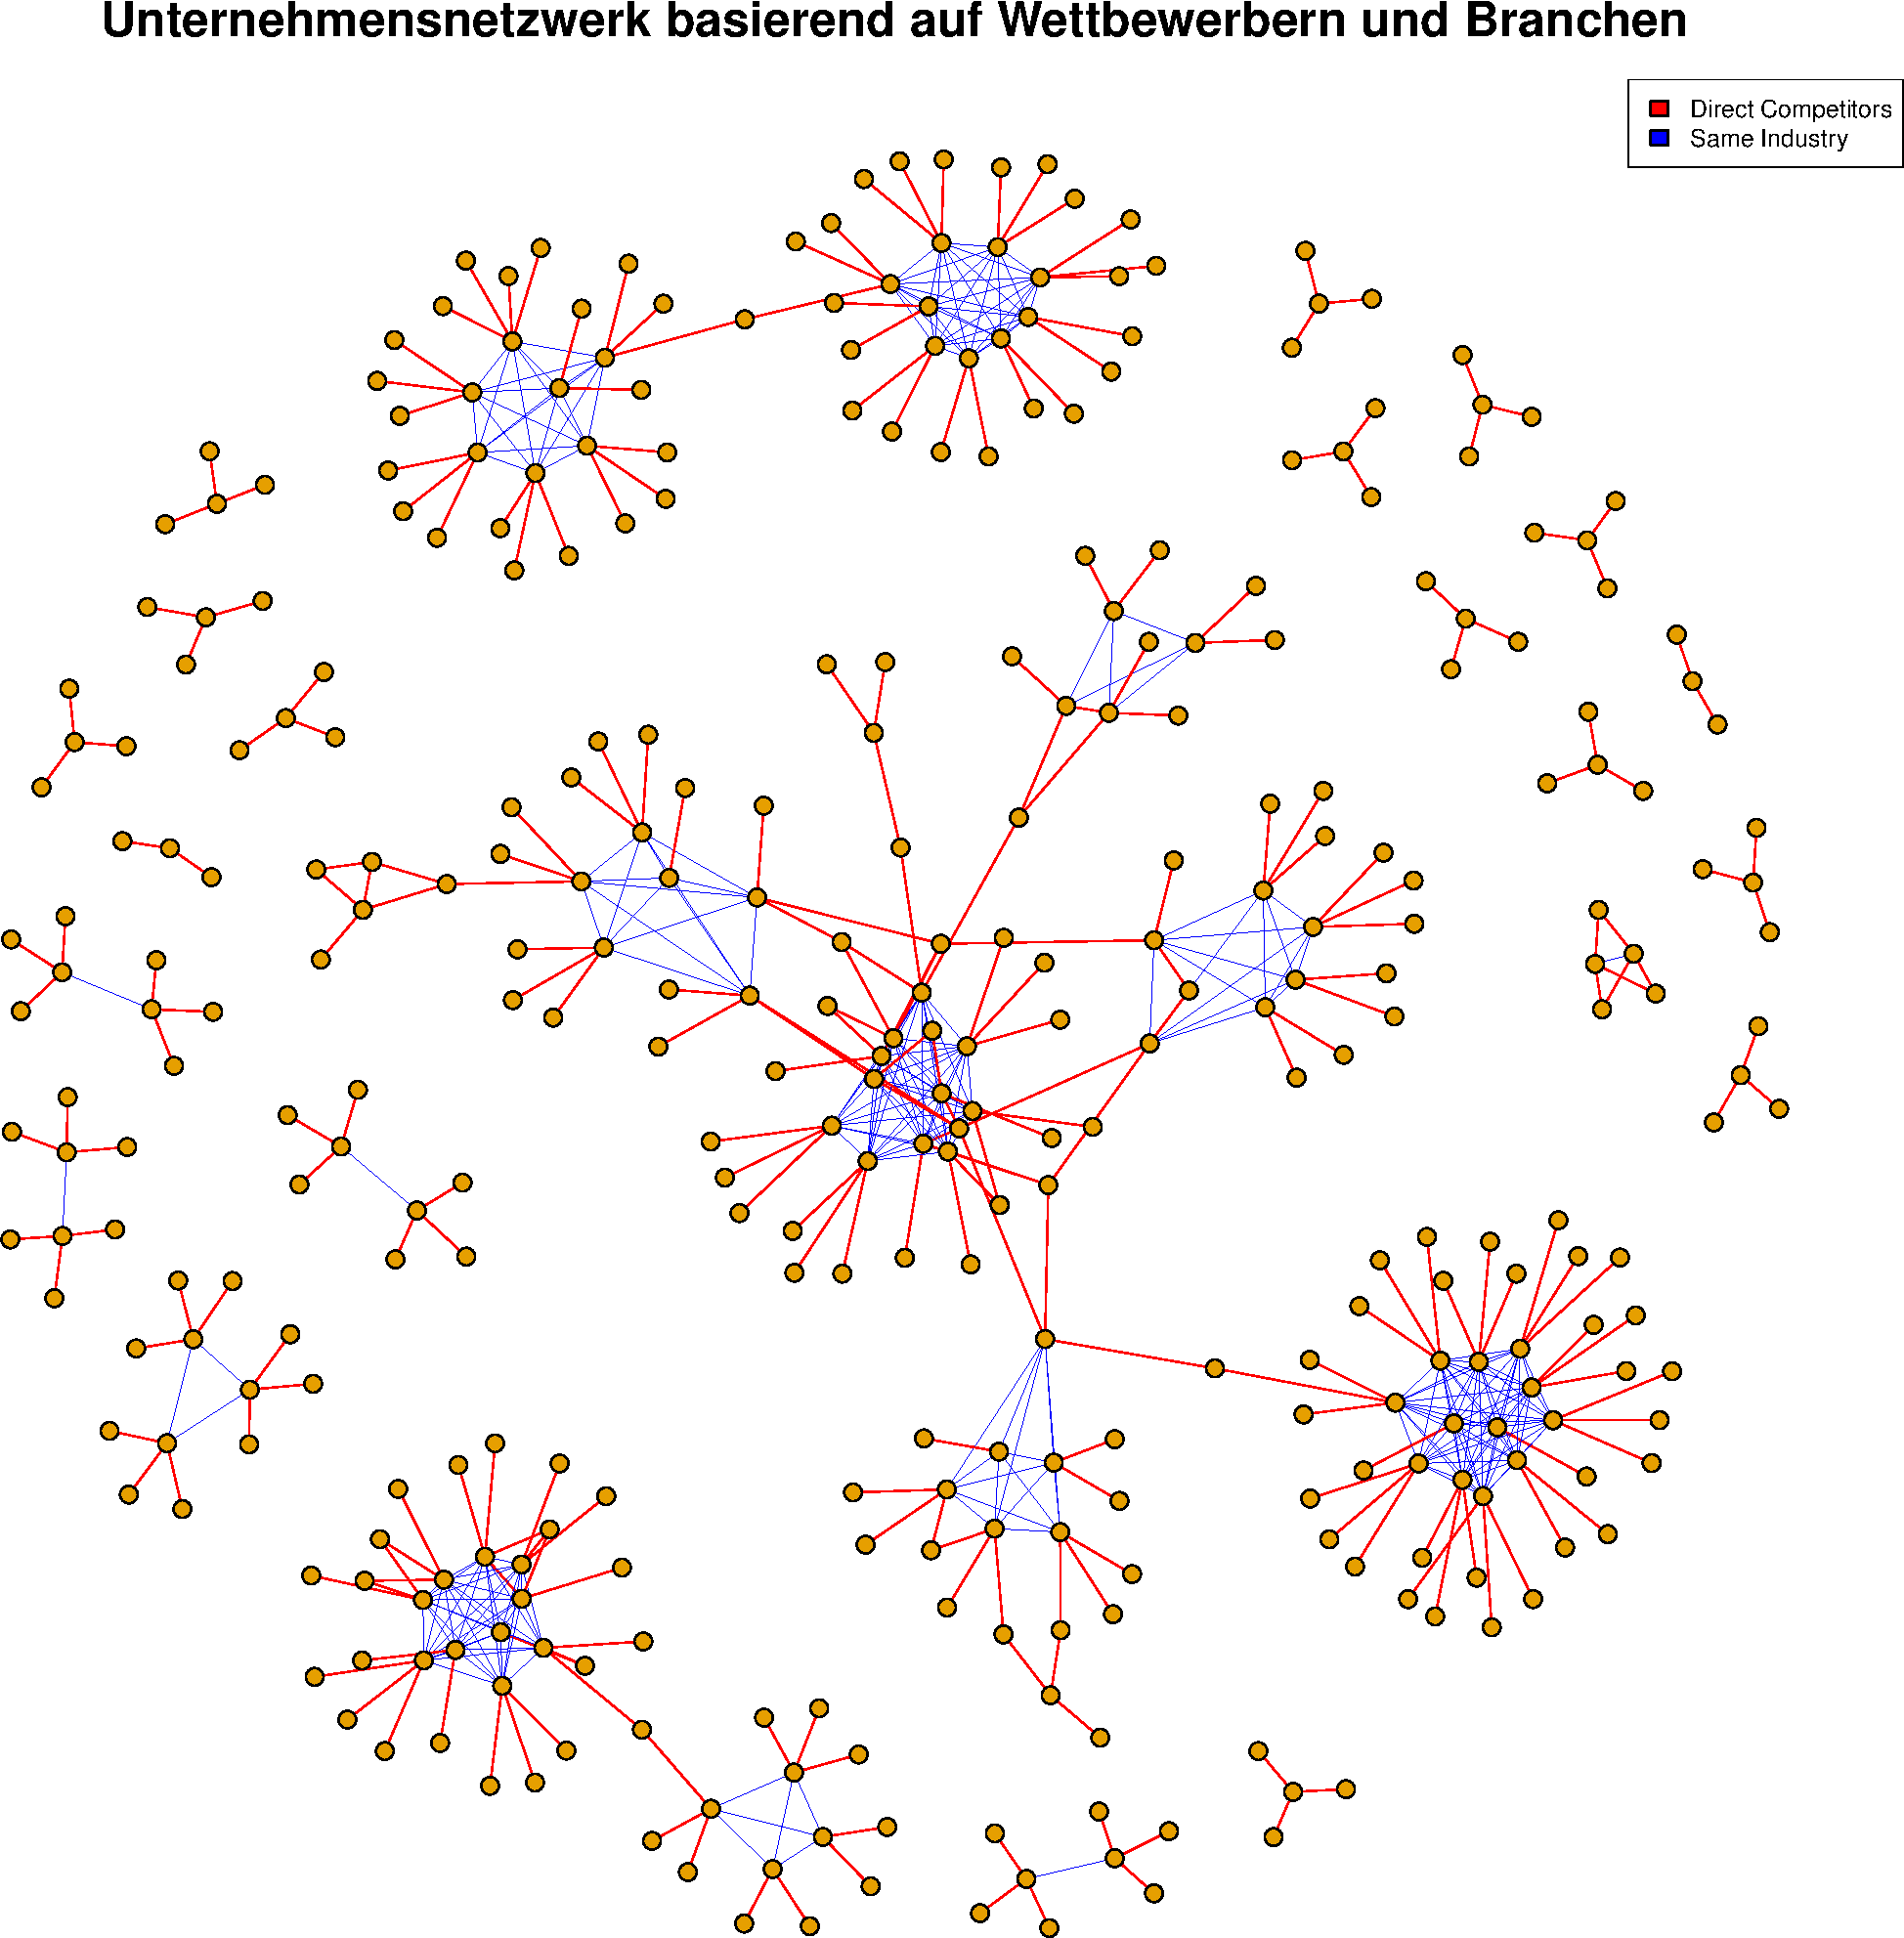
\includegraphics[keepaspectratio]{DataScience_files/figure-latex/unnamed-chunk-15-1.pdf}}
Es lassen sich einige interessante Beobachtungen aus dem Netzwerk
ziehen. Einerseits sind ganz eindeutig Branchencluster zu erkennen, die
auf die Branchenzugehörigkeit der Unternehmen hinweisen.

\begin{Shaded}
\begin{Highlighting}[]
\CommentTok{\# Ausgeben der 10 häufigsten Branchen im Netzwerk}
\NormalTok{top\_industries }\OtherTok{\textless{}{-}}\NormalTok{ data }\SpecialCharTok{\%\textgreater{}\%}
  \FunctionTok{count}\NormalTok{(Industry, }\AttributeTok{sort =} \ConstantTok{TRUE}\NormalTok{) }\SpecialCharTok{\%\textgreater{}\%}
  \FunctionTok{head}\NormalTok{(}\DecValTok{10}\NormalTok{)}

\CommentTok{\# Welche Unternehmen sind in mehreren Branchen vertreten?}
\NormalTok{multi\_industry\_companies }\OtherTok{\textless{}{-}}\NormalTok{ data }\SpecialCharTok{\%\textgreater{}\%}
  \FunctionTok{group\_by}\NormalTok{(}\StringTok{\textasciigrave{}}\AttributeTok{Company Name}\StringTok{\textasciigrave{}}\NormalTok{) }\SpecialCharTok{\%\textgreater{}\%}
  \FunctionTok{summarise}\NormalTok{(}\AttributeTok{Num\_Industries =} \FunctionTok{n\_distinct}\NormalTok{(Industry)) }\SpecialCharTok{\%\textgreater{}\%}
  \FunctionTok{filter}\NormalTok{(Num\_Industries }\SpecialCharTok{\textgreater{}} \DecValTok{1}\NormalTok{) }\SpecialCharTok{\%\textgreater{}\%}
  \FunctionTok{arrange}\NormalTok{(}\FunctionTok{desc}\NormalTok{(Num\_Industries))}

\CommentTok{\# Sind Unternehmen enthalten, die in mehreren Branchen vertreten sind?}
\ControlFlowTok{if}\NormalTok{ (}\FunctionTok{nrow}\NormalTok{(multi\_industry\_companies) }\SpecialCharTok{==} \DecValTok{0}\NormalTok{) \{}
  \FunctionTok{print}\NormalTok{(}\StringTok{"Keine Unternehmen in mehreren Branchen vertreten."}\NormalTok{)}
\NormalTok{\} }\ControlFlowTok{else}\NormalTok{ \{}
  \FunctionTok{print}\NormalTok{(}\StringTok{"Unternehmen in mehreren Branchen vertreten."}\NormalTok{)}
\NormalTok{\}}
\end{Highlighting}
\end{Shaded}

\begin{verbatim}
## [1] "Keine Unternehmen in mehreren Branchen vertreten."
\end{verbatim}

Jedoch sind keine Unternehmen in mehreren Branchen vertreten, was darauf
hindeutet, dass die Branchenzugehörigkeit eindeutig ist. Aber es gibt
einige Unternehmen, die mit direkter Konkurrenz die verschiedenen
Branchen verbinden. Dies könnte auf eine Diversifikation der
Geschäftsfelder hindeuten, die eine breitere Wettbewerbsbasis schafft.

Da aber wie oberhalb dargestellt, die Branchenzugehörigkeit eindeutig
ist, und somit die Branchenzugehörigkeit keinen Mehrwert für die Analyse
bietet, wird diese nicht weiter verfolgt.

\subsubsection{Betrachtung fokussiert auf direkte
Wettbewerber}\label{betrachtung-fokussiert-auf-direkte-wettbewerber}

Aus diesem Grund wird das Netzwerk auf direkte Wettbewerber beschränkt,
um die Analyse zu vereinfachen und die Relevanz der
Wettbewerbsbeziehungen zu erhöhen. \(\\\)

\begin{Shaded}
\begin{Highlighting}[]
\CommentTok{\# Extrahiere Unternehmen und ihre Wettbewerber}
\NormalTok{edges }\OtherTok{\textless{}{-}}\NormalTok{ data }\SpecialCharTok{\%\textgreater{}\%}
  \FunctionTok{separate\_rows}\NormalTok{(Competitors, }\AttributeTok{sep =} \StringTok{", "}\NormalTok{) }\SpecialCharTok{\%\textgreater{}\%}
  \FunctionTok{select}\NormalTok{(}\StringTok{\textasciigrave{}}\AttributeTok{Company Name}\StringTok{\textasciigrave{}}\NormalTok{, Competitors) }\SpecialCharTok{\%\textgreater{}\%}
  \FunctionTok{rename}\NormalTok{(}\AttributeTok{from =} \StringTok{\textasciigrave{}}\AttributeTok{Company Name}\StringTok{\textasciigrave{}}\NormalTok{, }\AttributeTok{to =}\NormalTok{ Competitors) }\SpecialCharTok{\%\textgreater{}\%}
  \FunctionTok{mutate}\NormalTok{(}\AttributeTok{weight =} \DecValTok{1}\NormalTok{)  }\CommentTok{\# Gewichtung für direkte Wettbewerber}

\CommentTok{\# Summiere die Gewichtungen für mehrere Kanten zwischen denselben Punkten}
\NormalTok{edge\_weights }\OtherTok{\textless{}{-}}\NormalTok{ edges }\SpecialCharTok{\%\textgreater{}\%}
  \FunctionTok{group\_by}\NormalTok{(from, to) }\SpecialCharTok{\%\textgreater{}\%}
  \FunctionTok{summarise}\NormalTok{(}\AttributeTok{weight =} \FunctionTok{sum}\NormalTok{(weight), }\AttributeTok{.groups =} \StringTok{\textquotesingle{}drop\textquotesingle{}}\NormalTok{)}

\CommentTok{\# Erstelle den Graphen nur mit direkten Wettbewerbern}
\NormalTok{g\_direct\_competitors }\OtherTok{\textless{}{-}} \FunctionTok{graph\_from\_data\_frame}\NormalTok{(edge\_weights, }\AttributeTok{directed =} \ConstantTok{FALSE}\NormalTok{)}

\CommentTok{\# Setze die Gewichtungen der Kanten im Graphen}
\FunctionTok{E}\NormalTok{(g\_direct\_competitors)}\SpecialCharTok{$}\NormalTok{weight }\OtherTok{\textless{}{-}}\NormalTok{ edge\_weights}\SpecialCharTok{$}\NormalTok{weight}

\CommentTok{\# Füge die Gehaltsdaten hinzu und berechne das durchschnittliche Gehalt pro Unternehmen}
\NormalTok{salary\_data }\OtherTok{\textless{}{-}}\NormalTok{ data }\SpecialCharTok{\%\textgreater{}\%}
  \FunctionTok{group\_by}\NormalTok{(}\StringTok{\textasciigrave{}}\AttributeTok{Company Name}\StringTok{\textasciigrave{}}\NormalTok{) }\SpecialCharTok{\%\textgreater{}\%}
  \FunctionTok{summarise}\NormalTok{(}\AttributeTok{AverageSalary =} \FunctionTok{mean}\NormalTok{(}\StringTok{\textasciigrave{}}\AttributeTok{Salary Estimate}\StringTok{\textasciigrave{}}\NormalTok{, }\AttributeTok{na.rm =} \ConstantTok{TRUE}\NormalTok{))}

\CommentTok{\# Füge die Gehaltsdaten zu den Knoten des Graphen hinzu}
\NormalTok{company\_names }\OtherTok{\textless{}{-}} \FunctionTok{V}\NormalTok{(g\_direct\_competitors)}\SpecialCharTok{$}\NormalTok{name}
\NormalTok{average\_salaries }\OtherTok{\textless{}{-}}\NormalTok{ salary\_data}\SpecialCharTok{$}\NormalTok{AverageSalary}
\NormalTok{company\_indices }\OtherTok{\textless{}{-}} \FunctionTok{match}\NormalTok{(company\_names, salary\_data}\SpecialCharTok{$}\StringTok{\textasciigrave{}}\AttributeTok{Company Name}\StringTok{\textasciigrave{}}\NormalTok{)}
\FunctionTok{V}\NormalTok{(g\_direct\_competitors)}\SpecialCharTok{$}\NormalTok{salary }\OtherTok{\textless{}{-}}\NormalTok{ average\_salaries[company\_indices]}

\CommentTok{\# Setze fehlende Gehaltsdaten auf einen speziellen Wert (z.B. 0)}
\FunctionTok{V}\NormalTok{(g\_direct\_competitors)}\SpecialCharTok{$}\NormalTok{salary[}\FunctionTok{is.na}\NormalTok{(}\FunctionTok{V}\NormalTok{(g\_direct\_competitors)}\SpecialCharTok{$}\NormalTok{salary)] }\OtherTok{\textless{}{-}} \DecValTok{0}

\CommentTok{\# Definiere die Gehaltsspektren}
\NormalTok{salary\_breaks }\OtherTok{\textless{}{-}} \FunctionTok{c}\NormalTok{(}\SpecialCharTok{{-}}\ConstantTok{Inf}\NormalTok{, }\DecValTok{50}\NormalTok{, }\DecValTok{80}\NormalTok{, }\DecValTok{100}\NormalTok{, }\DecValTok{150}\NormalTok{, }\ConstantTok{Inf}\NormalTok{)}
\NormalTok{salary\_labels }\OtherTok{\textless{}{-}} \FunctionTok{c}\NormalTok{(}\StringTok{"Lowest Salary"}\NormalTok{, }\StringTok{"Low Salary"}\NormalTok{, }\StringTok{"Medium Salary"}\NormalTok{, }\StringTok{"High Salary"}\NormalTok{,}
                   \StringTok{"Highest Salary"}\NormalTok{)}

\CommentTok{\# Setze die Farben der Knoten basierend auf den Gehältern}
\NormalTok{color\_palette }\OtherTok{\textless{}{-}} \FunctionTok{brewer.pal}\NormalTok{(}\DecValTok{5}\NormalTok{, }\StringTok{"YlOrRd"}\NormalTok{)}
\FunctionTok{V}\NormalTok{(g\_direct\_competitors)}\SpecialCharTok{$}\NormalTok{color }\OtherTok{\textless{}{-}} \FunctionTok{cut}\NormalTok{(}\FunctionTok{V}\NormalTok{(g\_direct\_competitors)}\SpecialCharTok{$}\NormalTok{salary,}
                                     \AttributeTok{breaks =}\NormalTok{ salary\_breaks,}
                                     \AttributeTok{labels =} \ConstantTok{FALSE}\NormalTok{, }
                                     \AttributeTok{include.lowest =} \ConstantTok{TRUE}\NormalTok{)}
\FunctionTok{V}\NormalTok{(g\_direct\_competitors)}\SpecialCharTok{$}\NormalTok{color }\OtherTok{\textless{}{-}}\NormalTok{ color\_palette[}\FunctionTok{V}\NormalTok{(g\_direct\_competitors)}\SpecialCharTok{$}\NormalTok{color]}

\CommentTok{\# Setze die Farben der Kanten basierend auf der Gewichtung}
\FunctionTok{E}\NormalTok{(g\_direct\_competitors)}\SpecialCharTok{$}\NormalTok{color }\OtherTok{\textless{}{-}} \StringTok{"red"}

\CommentTok{\# Visualisiere das Netzwerk mit kleineren Knoten}
\FunctionTok{plot}\NormalTok{(g\_direct\_competitors, }\AttributeTok{vertex.label =} \ConstantTok{NA}\NormalTok{,}
     \AttributeTok{vertex.size =} \DecValTok{3}\NormalTok{,  }\CommentTok{\# Kleinere Knoten}
     \AttributeTok{edge.width =} \DecValTok{1} \SpecialCharTok{*} \FunctionTok{E}\NormalTok{(g\_direct\_competitors)}\SpecialCharTok{$}\NormalTok{weight,}\CommentTok{\# Reduzierte Gewichtung der Kanten}
     \AttributeTok{edge.arrow.size =} \DecValTok{1}\NormalTok{,}
     \AttributeTok{layout =}\NormalTok{ layout\_with\_fr}
\NormalTok{)}
\FunctionTok{title}\NormalTok{(}\AttributeTok{main =} \StringTok{"Unternehmensnetzwerk basierend auf direkten Wettbewerbern"}\NormalTok{, }\AttributeTok{cex.main =} \DecValTok{2}\NormalTok{)}

\CommentTok{\# Legende für Knotenfarben}
\FunctionTok{legend}\NormalTok{(}\StringTok{"topright"}\NormalTok{, }\AttributeTok{legend =}\NormalTok{ salary\_labels,}
       \AttributeTok{fill =}\NormalTok{ color\_palette)}
\end{Highlighting}
\end{Shaded}

\pandocbounded{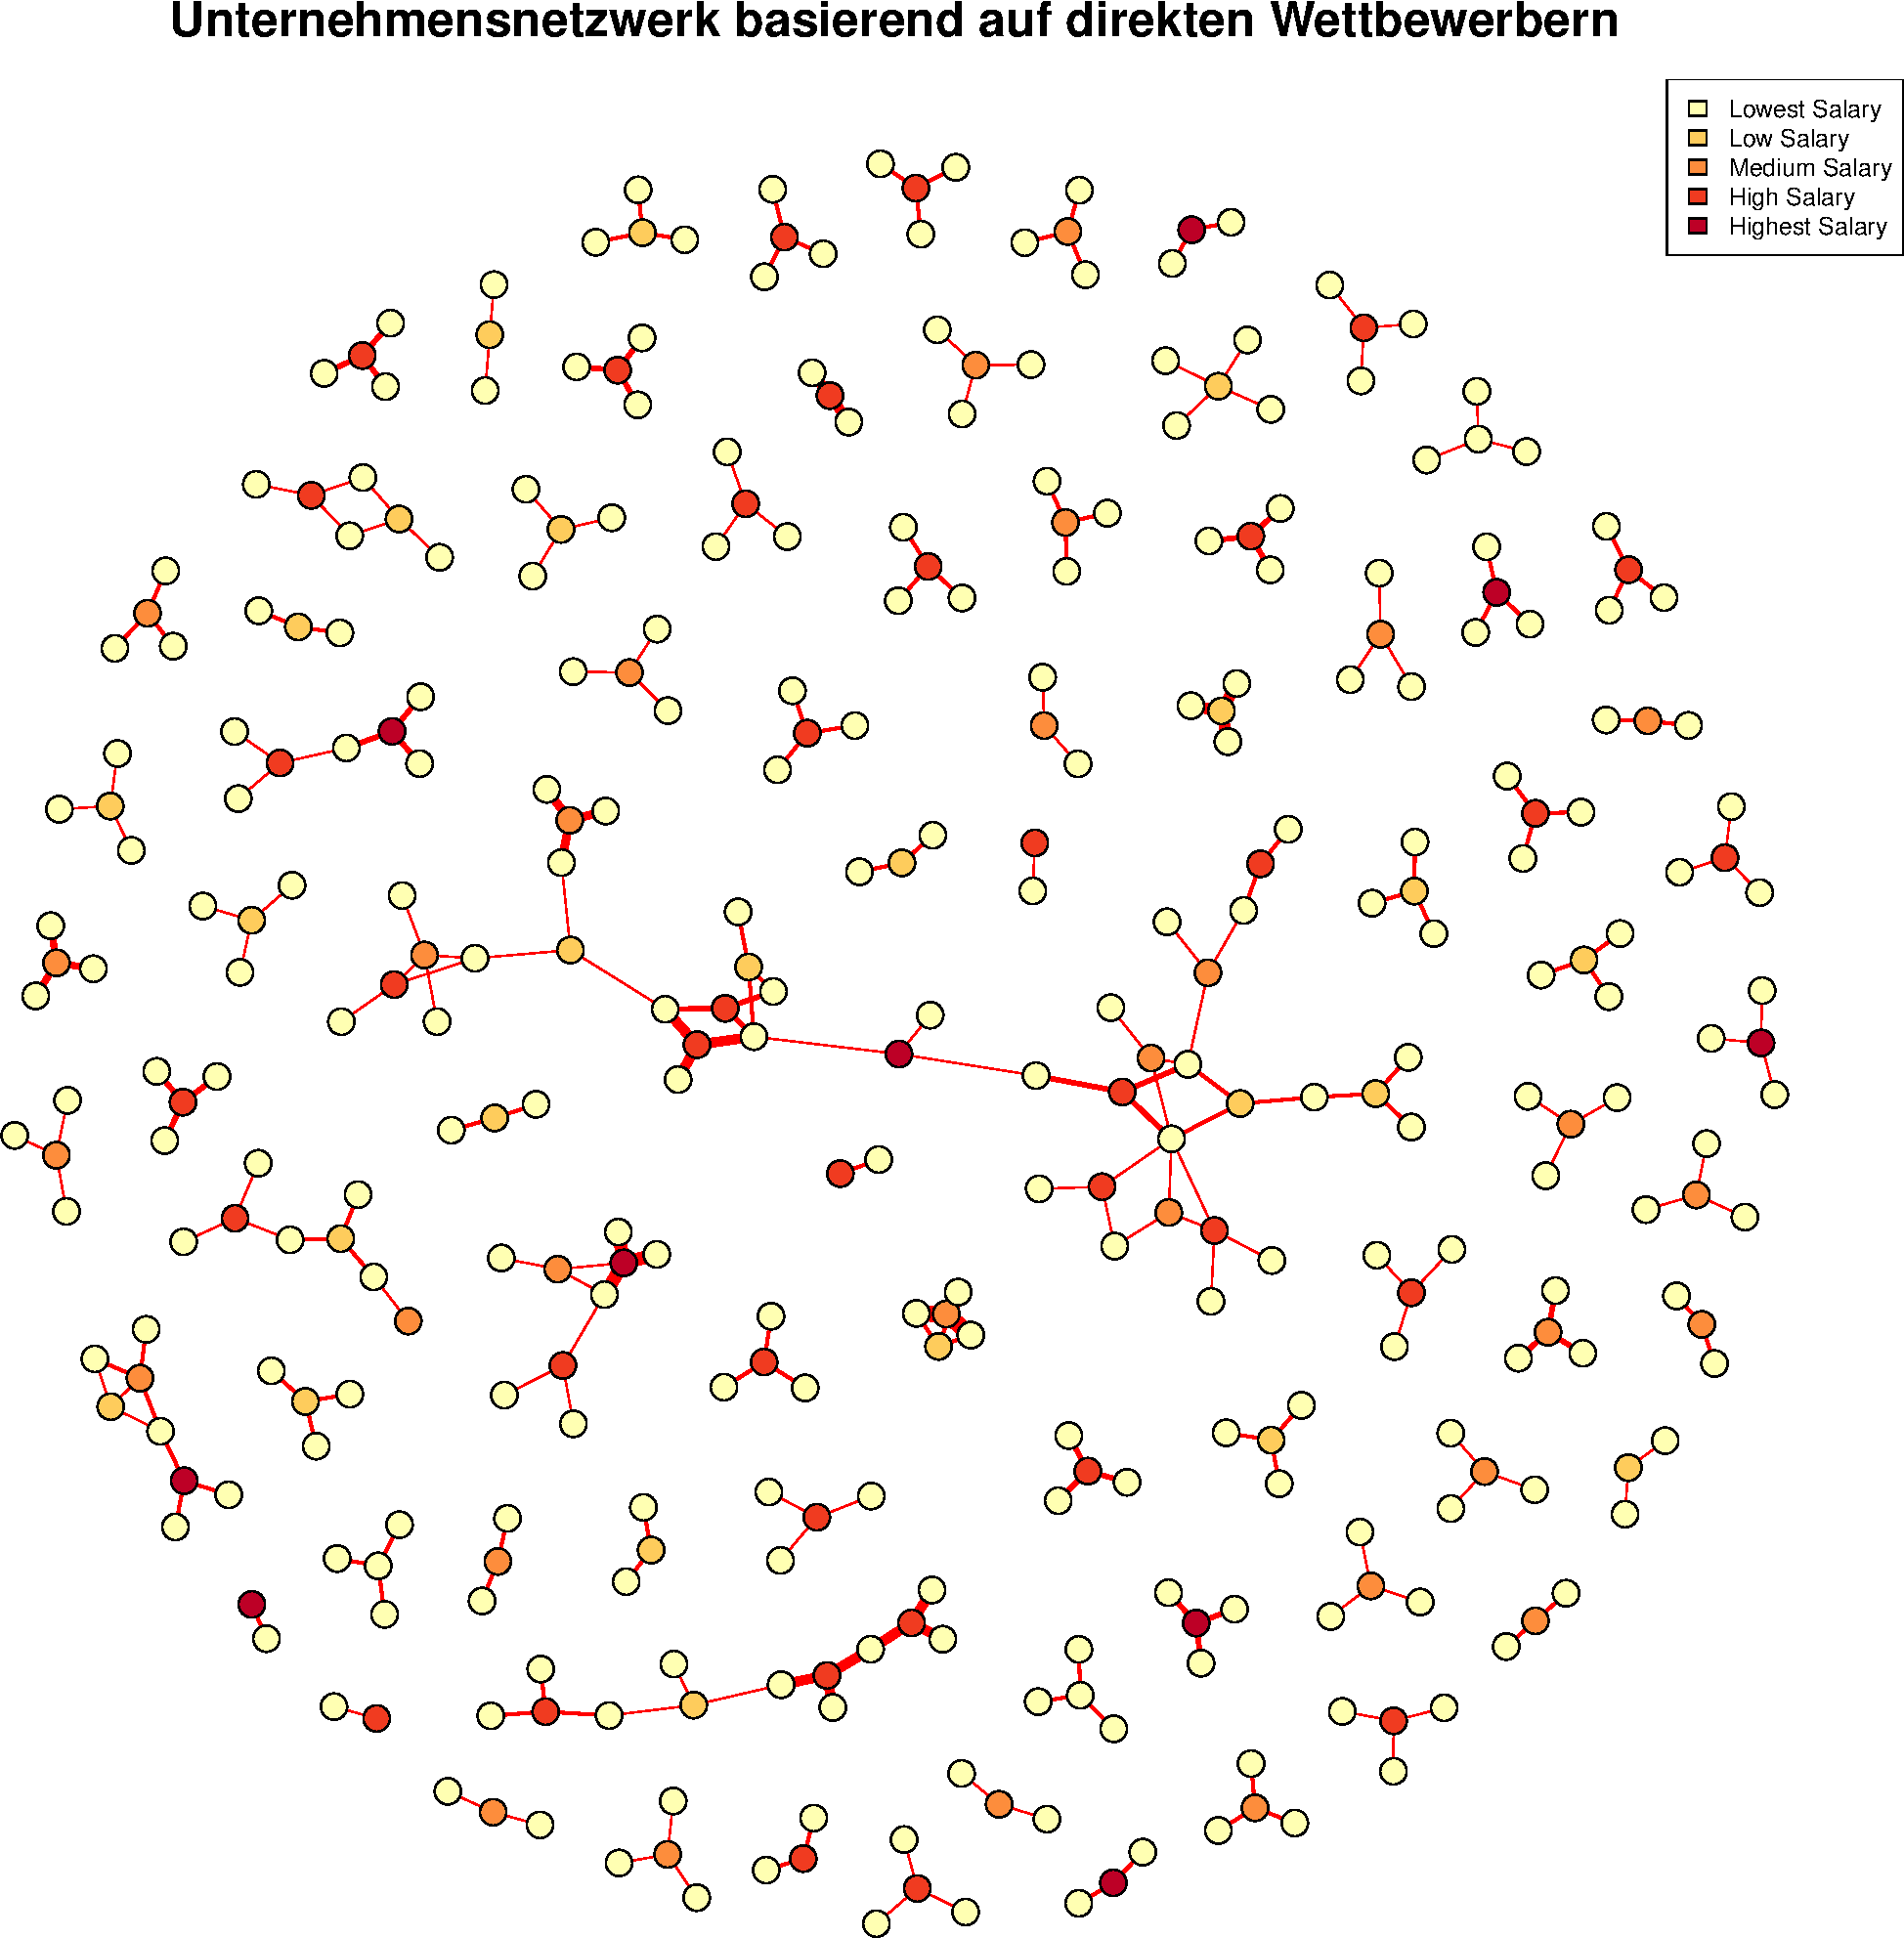
\includegraphics[keepaspectratio]{DataScience_files/figure-latex/unnamed-chunk-17-1.pdf}}

\begin{Shaded}
\begin{Highlighting}[]
\CommentTok{\# Ausgabe der Gehälter der Unternehmen}
\NormalTok{salary\_data }\OtherTok{\textless{}{-}}\NormalTok{ data }\SpecialCharTok{\%\textgreater{}\%}
  \FunctionTok{group\_by}\NormalTok{(}\StringTok{\textasciigrave{}}\AttributeTok{Company Name}\StringTok{\textasciigrave{}}\NormalTok{) }\SpecialCharTok{\%\textgreater{}\%}
  \FunctionTok{summarise}\NormalTok{(}\AttributeTok{AverageSalary =} \FunctionTok{mean}\NormalTok{(}\StringTok{\textasciigrave{}}\AttributeTok{Salary Estimate}\StringTok{\textasciigrave{}}\NormalTok{, }\AttributeTok{na.rm =} \ConstantTok{TRUE}\NormalTok{)) }\SpecialCharTok{\%\textgreater{}\%}
  \FunctionTok{arrange}\NormalTok{(}\FunctionTok{desc}\NormalTok{(AverageSalary))}

\CommentTok{\# Ausgabe der 10 Unternehmen mit den höchsten Gehältern}
\FunctionTok{print}\NormalTok{(salary\_data, }\AttributeTok{n =} \DecValTok{10}\NormalTok{)}
\end{Highlighting}
\end{Shaded}

\begin{verbatim}
## # A tibble: 107 x 2
##    `Company Name`           AverageSalary
##    <chr>                            <dbl>
##  1 Gallup                            238.
##  2 Credit Sesame                     205 
##  3 The Climate Corporation           194 
##  4 Liberty Mutual Insurance          179.
##  5 Samsung Research America          177 
##  6 Western Digital                   172.
##  7 Glassdoor                         162 
##  8 Netskope                          154.
##  9 Factual                           153 
## 10 Visa Inc.                         153.
## # i 97 more rows
\end{verbatim}

\begin{Shaded}
\begin{Highlighting}[]
\CommentTok{\# Konkrete Gehaltsspektren für die jeweilige Färbung}
\FunctionTok{print}\NormalTok{(}\StringTok{"Gehaltsspektren für die jeweilige Färbung:"}\NormalTok{)}
\end{Highlighting}
\end{Shaded}

\begin{verbatim}
## [1] "Gehaltsspektren für die jeweilige Färbung:"
\end{verbatim}

\begin{Shaded}
\begin{Highlighting}[]
\FunctionTok{print}\NormalTok{(salary\_breaks)}
\end{Highlighting}
\end{Shaded}

\begin{verbatim}
## [1] -Inf   50   80  100  150  Inf
\end{verbatim}

Das Unternehmensnetzwerk demonstriert die engen Verbindungen zwischen
Unternehmen, die auf direkten Wettbewerbsbeziehungen basieren, und
stellt dabei die Gehälter der Unternehmen heraus. Die Farbe der Knoten
variiert entsprechend den Gehaltsniveaus. Dabei werden niedrige Gehälter
durch hellgelb und höhere Gehälter durch rote bsi dunkelrote Farben
symbolisiert.

In der Mitte des Netzwerks lassen sich einige Unternehmen mit hohen
Gehältern und zahlreichen Verbindungen ausmachen, die eine zentrale Lage
einnehmen (dunkelrot). Es lässt sich vermuten, dass diese Unternehmen
eine zentrale Rolle im Wettbewerbsnetzwerk einnehmen. Dies könnte darauf
hindeuten, dass sie dominierende Marktakteure oder wichtige
Branchenführer sind.

Das Netzwerk ist gekennzeichnet durch eine Vielzahl kleinerer, weniger
vernetzter Unternehmenscluster, die tendenziell niedrigere Gehälter
zahlen (hellere Farben). Die Präsenz peripherer Gruppen könnte darauf
hinweisen, dass es sich um Nischenmärkte oder weniger stark umkämpfte
Branchen handelt.

Allgemein lässt sich jedoch feststellen, dass Unternehmen die sich in
einer zentraleren Positionen innerhalb ihres Clusters befinden, im
Durchschnitt deutlich höhere Gehälter anbieten. Dies lässt den Schluss
zu, dass eine stärkere Wettbewerbsposition sowie eine höhere
Attraktivität für qualifizierte Arbeitskräfte gegeben sind.

\subsection{Zentralitätsanalyse innerhalb des
Netzwerkes}\label{zentralituxe4tsanalyse-innerhalb-des-netzwerkes}

Die hier präsentierten Zentralitätsmaße lassen sich unmittelbar auf die
Gehaltsstrukturen im Kontext des Wettbewerbsnetzwerks anwenden. Auf
diese Weise könnten sie dazu beitragen, die Position eines Unternehmens
in Bezug auf seine Wettbewerber hinsichtlich der Gehälter zu bestimmen.
\(\\\) Folgend wird die Berechnung der Zentralitätsmaße für die
Unternehmen im Wettbewerbsnetzwerk dargelegt. \(\\\)

\begin{Shaded}
\begin{Highlighting}[]
\CommentTok{\# Datenauswahl für die Zentralitätsanalyse}
\NormalTok{selected\_data }\OtherTok{\textless{}{-}}\NormalTok{ data }\SpecialCharTok{\%\textgreater{}\%}
  \FunctionTok{select}\NormalTok{(}\StringTok{\textasciigrave{}}\AttributeTok{Company Name}\StringTok{\textasciigrave{}}\NormalTok{, Competitors, }\StringTok{\textasciigrave{}}\AttributeTok{Salary Estimate}\StringTok{\textasciigrave{}}\NormalTok{)}

\CommentTok{\# Extrahiere Unternehmen und ihre Wettbewerber}
\NormalTok{edges }\OtherTok{\textless{}{-}}\NormalTok{ selected\_data }\SpecialCharTok{\%\textgreater{}\%}
  \FunctionTok{separate\_rows}\NormalTok{(Competitors, }\AttributeTok{sep =} \StringTok{", "}\NormalTok{) }\SpecialCharTok{\%\textgreater{}\%}
  \FunctionTok{select}\NormalTok{(}\StringTok{\textasciigrave{}}\AttributeTok{Company Name}\StringTok{\textasciigrave{}}\NormalTok{, Competitors) }\SpecialCharTok{\%\textgreater{}\%}
  \FunctionTok{rename}\NormalTok{(}\AttributeTok{from =} \StringTok{\textasciigrave{}}\AttributeTok{Company Name}\StringTok{\textasciigrave{}}\NormalTok{, }\AttributeTok{to =}\NormalTok{ Competitors)}

\CommentTok{\# Erstelle den Graphen}
\NormalTok{g\_competitors\_zentralität }\OtherTok{\textless{}{-}} \FunctionTok{graph\_from\_data\_frame}\NormalTok{(edges, }\AttributeTok{directed =} \ConstantTok{FALSE}\NormalTok{)}


\CommentTok{\# Berechne die Zentralitätsmaße für die Knoten}
\NormalTok{degree\_centrality }\OtherTok{\textless{}{-}} \FunctionTok{degree}\NormalTok{(g\_competitors\_zentralität, }\AttributeTok{mode =} \StringTok{"all"}\NormalTok{)}
\NormalTok{betweenness\_centrality }\OtherTok{\textless{}{-}} \FunctionTok{betweenness}\NormalTok{(g\_competitors\_zentralität, }\AttributeTok{directed =} \ConstantTok{FALSE}\NormalTok{)}
\NormalTok{eigenvector\_centrality }\OtherTok{\textless{}{-}} \FunctionTok{evcent}\NormalTok{(g\_competitors\_zentralität, }\AttributeTok{directed =} \ConstantTok{FALSE}\NormalTok{)}
\end{Highlighting}
\end{Shaded}

\begin{verbatim}
## Warning: `evcent()` was deprecated in igraph 2.0.0.
## i Please use `eigen_centrality()` instead.
## This warning is displayed once every 8 hours.
## Call `lifecycle::last_lifecycle_warnings()` to see where this warning was
## generated.
\end{verbatim}

\subsubsection{Betweenness-Zentralität}\label{betweenness-zentralituxe4t}

Jetzt soll das igraph-Paket in R verwendet werden, um die
Betweenness-Zentralität für jeden Knoten zu berechnen. Unternehmen mit
hoher Betweenness-Centralität könnten strategische Wettbewerbsvorteile
aufweisen, da sie als Vermittler zwischen mehreren Konkurrenten
fungieren und dadurch den Informationsfluss beeinflussen können. \(\\\)
Die Unternehmen könnten höhere Gehälter anbieten, um hochqualifizierte
Arbeitskräfte zu gewinnen, die dazu beitragen, ihre zentrale Position
und die damit verbundenen Wettbewerbsvorteile zu erhalten. Alternativ
könnte ein hohes Gehalt auch als Indikator für eine hohe Nachfrage nach
qualifizierten Mitarbeitenden in solchen Schlüsselpositionen dienen, da
das Unternehmen sich in einem Bereich positioniert, der viele
strategische Informationen benötigt.

\begin{Shaded}
\begin{Highlighting}[]
\CommentTok{\# Berechne die Betweenness{-}Centrality und sortiere sie absteigend}
\NormalTok{top\_betweenness }\OtherTok{\textless{}{-}} \FunctionTok{head}\NormalTok{(}\FunctionTok{sort}\NormalTok{(betweenness\_centrality, }\AttributeTok{decreasing =} \ConstantTok{TRUE}\NormalTok{), }\DecValTok{5}\NormalTok{)}

\CommentTok{\# Erstelle ein DataFrame mit den Namen der Unternehmen und ihrer Betweenness{-}Centrality}
\NormalTok{top\_betweenness\_df }\OtherTok{\textless{}{-}} \FunctionTok{data.frame}\NormalTok{(}
  \AttributeTok{Company =} \FunctionTok{names}\NormalTok{(top\_betweenness),}
  \AttributeTok{Betweenness =} \FunctionTok{as.numeric}\NormalTok{(top\_betweenness),}
  \AttributeTok{stringsAsFactors =} \ConstantTok{FALSE}
\NormalTok{)}

\CommentTok{\# Erstellen einer Tabelle}
\FunctionTok{kable}\NormalTok{(top\_betweenness\_df, }\AttributeTok{format =} \StringTok{"latex"}\NormalTok{, }\AttributeTok{booktabs =} \ConstantTok{TRUE}\NormalTok{, }\AttributeTok{align =} \StringTok{"l"}\NormalTok{) }\SpecialCharTok{\%\textgreater{}\%}
\FunctionTok{kable\_styling}\NormalTok{(}\AttributeTok{latex\_options =} \FunctionTok{c}\NormalTok{(}\StringTok{"striped"}\NormalTok{, }\StringTok{"hold\_position"}\NormalTok{), }\AttributeTok{position =} \StringTok{"left"}\NormalTok{)}
\end{Highlighting}
\end{Shaded}

\begin{tabular}{ll}
\toprule
Company & Betweenness\\
\midrule
\cellcolor{gray!10}{PA Consulting} & \cellcolor{gray!10}{492.8571}\\
Gallup & 479.0000\\
\cellcolor{gray!10}{Booz Allen Hamilton} & \cellcolor{gray!10}{477.1818}\\
McKinsey \& Company & 462.0000\\
\cellcolor{gray!10}{General Dynamics Information Technology} & \cellcolor{gray!10}{354.0000}\\
\bottomrule
\end{tabular}

\(\\\)

\begin{Shaded}
\begin{Highlighting}[]
\CommentTok{\# Zusammenhang zwischen durchschnittliches Gehalt und Betweenness{-}Zentralität}
\NormalTok{salary\_betweenness }\OtherTok{\textless{}{-}} \FunctionTok{data.frame}\NormalTok{(}
  \AttributeTok{Salary =}\NormalTok{ salary\_data}\SpecialCharTok{$}\NormalTok{AverageSalary,}
  \AttributeTok{Betweenness =}\NormalTok{ betweenness\_centrality[}
    \FunctionTok{match}\NormalTok{(salary\_data}\SpecialCharTok{$}\StringTok{\textasciigrave{}}\AttributeTok{Company Name}\StringTok{\textasciigrave{}}\NormalTok{, }\FunctionTok{names}\NormalTok{(betweenness\_centrality))}
\NormalTok{  ]}
\NormalTok{)}

\CommentTok{\# Scatterplot mit roter, gestrichelter Trendlinie}
\FunctionTok{ggplot}\NormalTok{(salary\_betweenness, }\FunctionTok{aes}\NormalTok{(}\AttributeTok{x =}\NormalTok{ Salary, }\AttributeTok{y =}\NormalTok{ Betweenness)) }\SpecialCharTok{+}
  \FunctionTok{geom\_point}\NormalTok{() }\SpecialCharTok{+}
  \FunctionTok{geom\_smooth}\NormalTok{(}\AttributeTok{method =} \StringTok{"loess"}\NormalTok{, }\AttributeTok{se =} \ConstantTok{FALSE}\NormalTok{, }\AttributeTok{color =} \StringTok{"red"}\NormalTok{, }\AttributeTok{linetype =} \StringTok{"dashed"}\NormalTok{) }\SpecialCharTok{+}
  \FunctionTok{labs}\NormalTok{(}\AttributeTok{title =} \StringTok{"Scatterplot of Salary vs. Betweenness Centrality"}\NormalTok{,}
       \AttributeTok{x =} \StringTok{"Salary"}\NormalTok{, }\AttributeTok{y =} \StringTok{"Betweenness Centrality"}\NormalTok{) }\SpecialCharTok{+}
  \FunctionTok{theme\_minimal}\NormalTok{() }\SpecialCharTok{+}
  \FunctionTok{theme}\NormalTok{(}
    \AttributeTok{plot.title =} \FunctionTok{element\_text}\NormalTok{(}\AttributeTok{size =} \DecValTok{14}\NormalTok{, }\AttributeTok{face =} \StringTok{"bold"}\NormalTok{),}
    \AttributeTok{axis.title =} \FunctionTok{element\_text}\NormalTok{(}\AttributeTok{size =} \DecValTok{12}\NormalTok{, }\AttributeTok{face =} \StringTok{"bold"}\NormalTok{),}
    \AttributeTok{axis.text =} \FunctionTok{element\_text}\NormalTok{(}\AttributeTok{size =} \DecValTok{12}\NormalTok{)}
\NormalTok{  )}
\end{Highlighting}
\end{Shaded}

\begin{verbatim}
## `geom_smooth()` using formula = 'y ~ x'
\end{verbatim}

\pandocbounded{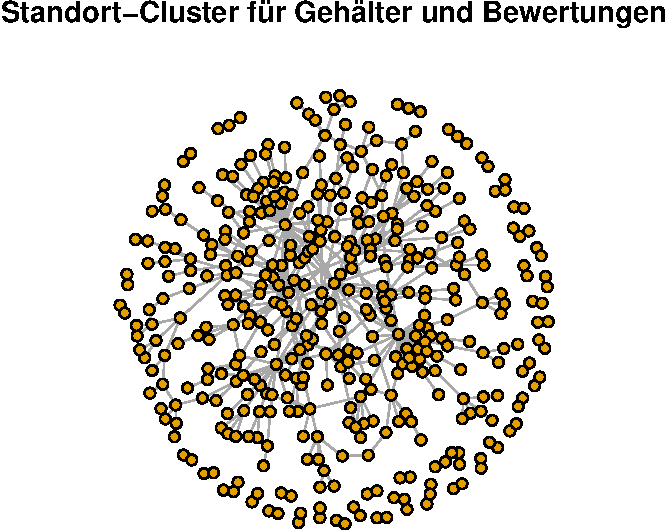
\includegraphics[keepaspectratio]{DataScience_files/figure-latex/unnamed-chunk-20-1.pdf}}
Der Scatterplot veranschaulicht die Korrelation zwischen dem Gehalt auf
der x-Achse und der Betweenness Centrality auf der y-Achse. Die rote
Linie zeigt einen nichtlinearen Trend zwischen Gehalt und Betweenness
Centrality, was auf eine mögliche Korrelation hinweisen könnte,
insbesondere bei höheren Gehältern.

Die Mehrzahl der Unternehmen weist eine geringe Betweenness Centrality
auf, wobei die Höhe der Vergütung eine eher untergeordnete Rolle spielt.
Allerdings lässt sich eine Ausnahmen beobachten. Ab ca. 150k Dollar auf
der Gehaltsachse zeigt der Trend einen deutlichen Anstieg der
Betweenness Centrality. Dies könnte bedeuten, dass Unternehmen mit sehr
hohen Gehältern tendenziell auch höhere Betweenness Centrality Werte
aufweisen und somit eine wichtige Vermittlerrolle im Netzwerk einnehmen.
Jedoch wird dieser Antieg bloß von einem Unternehmen repräsentiert, was
auf eine Ausnahme hinweisen könnte. Dieses Unternehmen könnten jedoch
ein besonders attraktiver Arbeitgeber für strategische
Schlüsselpositionen sein und durch hohe Gehälter zusätzlich Talente
anziehen.

Allgemiens lässt dies den Schluss zu, dass bestimmte Unternehmen eine
zentrale Vermittlerrolle im Netzwerk einnehmen, ohne zwangsläufig die
höchsten Gehälter zu offerieren.

Die wenigen Unternehmen mit einer sehr hohen Betweenness Centrality
könnten als strategische Vermittler im Markt auftreten und dabei
möglicherweise andere Vorteile nutzen, anstatt ihre Gehälter zu erhöhen.
Die dargelegte Erkenntnis lässt die Hypothese zu, dass Unternehmen, die
über zahlreiche Verbindungen im Wettbewerbsnetzwerk verfügen, ihre
Attraktivität nicht allein durch monetäre Zuwendungen, sondern auch
durch andere Vorteile oder Reputation aufrechterhalten könnten. Für
hochspezialisierte Unternehmen, die in einer Nische tätig sind und
weniger Konkurrenz haben, könnte es sich lohnen, gezielt in Gehälter zu
investieren, um Talente anzuziehen.

Im folgenden Schritt soll sich der Außreißer mit dem höchsten Gehalt und
der zweithöchsten Betweenness Centrality genauer betrachtet werden.

\begin{Shaded}
\begin{Highlighting}[]
\CommentTok{\# Unternehmen mit dem höchsten Gehalt und der zweithöchsten Betweenness Centrality}
\NormalTok{outlier }\OtherTok{\textless{}{-}}\NormalTok{ salary\_betweenness }\SpecialCharTok{\%\textgreater{}\%}
  \FunctionTok{filter}\NormalTok{(Salary }\SpecialCharTok{\textgreater{}} \DecValTok{210} \SpecialCharTok{\&}\NormalTok{ Betweenness }\SpecialCharTok{\textgreater{}} \FloatTok{0.0001}\NormalTok{)}

\CommentTok{\# Ausgabe des Unternehmens}
\FunctionTok{print}\NormalTok{(outlier)}
\end{Highlighting}
\end{Shaded}

\begin{verbatim}
##        Salary Betweenness
## Gallup  237.5         479
\end{verbatim}

\(\\\) Das Unternehmen mit dem höchsten Gehalt und der zweithöchsten
Betweenness Centrality ist ``Gallup''. \(\\\)

\begin{Shaded}
\begin{Highlighting}[]
\CommentTok{\# Berechne die Nachbarn von "Gallup"}
\NormalTok{gallup\_neighbors }\OtherTok{\textless{}{-}} \FunctionTok{neighbors}\NormalTok{(g\_direct\_competitors, }\StringTok{"Gallup"}\NormalTok{, }\AttributeTok{mode =} \StringTok{"all"}\NormalTok{)}

\CommentTok{\# Erstelle ein DataFrame mit den Namen der direkten Wettbewerber von "Gallup"}
\NormalTok{gallup\_neighbors\_df }\OtherTok{\textless{}{-}} \FunctionTok{data.frame}\NormalTok{(}
  \AttributeTok{Competitors =} \FunctionTok{names}\NormalTok{(gallup\_neighbors),}
  \AttributeTok{stringsAsFactors =} \ConstantTok{FALSE}
\NormalTok{)}

\CommentTok{\# Erstelle eine schön formatierte Tabelle im LaTeX{-}Format}
\FunctionTok{kable}\NormalTok{(gallup\_neighbors\_df, }\AttributeTok{format =} \StringTok{"latex"}\NormalTok{, }\AttributeTok{booktabs =} \ConstantTok{TRUE}\NormalTok{, }\AttributeTok{align =} \StringTok{"l"}\NormalTok{) }\SpecialCharTok{\%\textgreater{}\%}
  \FunctionTok{kable\_styling}\NormalTok{(}\AttributeTok{latex\_options =} \FunctionTok{c}\NormalTok{(}\StringTok{"striped"}\NormalTok{, }\StringTok{"hold\_position"}\NormalTok{), }\AttributeTok{position =} \StringTok{"left"}\NormalTok{) }\SpecialCharTok{\%\textgreater{}\%}
  \FunctionTok{column\_spec}\NormalTok{(}\DecValTok{1}\NormalTok{, }\AttributeTok{width =} \StringTok{"5cm"}\NormalTok{)}
\end{Highlighting}
\end{Shaded}

\begin{tabular}{>{\raggedright\arraybackslash}p{5cm}}
\toprule
Competitors\\
\midrule
\cellcolor{gray!10}{Booz Allen Hamilton}\\
Advisory Board\\
\cellcolor{gray!10}{McKinsey \& Company}\\
\bottomrule
\end{tabular}

\(\\\) ``Gallup'' hat 3 direkte Wettbewerber: ``Booz Allen Hamilton'',
``Advisory Board'' und ``McKinsey \& Company''. Daraus lässt sich
schließen, dass ``Gallup'' eine zentrale Vermittlerrolle zwischen diesen
drei Unternehmen einnimmt, was durch die hohe Betweenness Centrality und
das hohe Gehalt reflektiert wird.

\subsubsection{Degree-Zentralität}\label{degree-zentralituxe4t}

Hier wird die Anzahl der Kanten gezählt, die an jedem Knoten hängen.
Hohe Werte können auf starke Verbindungen zu anderen Unternehmen
hinweisen. Unternehmen mit hoher Degree Centrality sind also in einem
besonderem Maße der Konkurrenz durch eine Vielzahl anderer Firmen
ausgesetzt, was zu einem hohen Druck innerhalb der Branche führen kann.

Ein hoher Degree Centrality-Wert lässt die Vermutung zu, dass es sich um
ein Unternehmen handelt, welches sich durch höhere Gehälter von der
Konkurrenz abheben und somit Talente anwerben möchte. Andererseits
besteht für Unternehmen in stark besetzten Märkten die Möglichkeit,
durch Maßnahmen wie eine attraktive Arbeitskultur oder
Weiterbildungsmöglichkeiten für Mitarbeiter, trotz eines geringeren
Gehalts, für Bewerber attraktiver zu sein. In diesem Fall können
Unternehmen mit mittleren oder niedrigeren Degree-Centrality-Werten im
Vergleich attraktivere Gehälter bieten, da sie weniger Wettbewerbsdruck
haben und gezielt in Gehälter investieren können.

\begin{Shaded}
\begin{Highlighting}[]
\CommentTok{\# Berechne die Degree{-}Centrality und sortiere sie absteigend}
\NormalTok{top\_degree }\OtherTok{\textless{}{-}} \FunctionTok{head}\NormalTok{(}\FunctionTok{sort}\NormalTok{(degree\_centrality, }\AttributeTok{decreasing =} \ConstantTok{TRUE}\NormalTok{), }\DecValTok{5}\NormalTok{)}

\CommentTok{\# Erstelle ein DataFrame mit den Namen der Unternehmen und ihrer Degree{-}Centrality}
\NormalTok{top\_degree\_df }\OtherTok{\textless{}{-}} \FunctionTok{data.frame}\NormalTok{(}
  \AttributeTok{Company =} \FunctionTok{names}\NormalTok{(top\_degree),}
  \AttributeTok{Degree =} \FunctionTok{as.numeric}\NormalTok{(top\_degree),}
  \AttributeTok{stringsAsFactors =} \ConstantTok{FALSE}
\NormalTok{)}

\CommentTok{\# Erstelle die Tabelle und zentriere sie links}
\FunctionTok{kable}\NormalTok{(gallup\_neighbors\_df, }\AttributeTok{format =} \StringTok{"latex"}\NormalTok{, }\AttributeTok{booktabs =} \ConstantTok{TRUE}\NormalTok{, }\AttributeTok{align =} \StringTok{"l"}\NormalTok{) }\SpecialCharTok{\%\textgreater{}\%}
  \FunctionTok{kable\_styling}\NormalTok{(}\AttributeTok{latex\_options =} \FunctionTok{c}\NormalTok{(}\StringTok{"striped"}\NormalTok{, }\StringTok{"hold\_position"}\NormalTok{), }\AttributeTok{position =} \StringTok{"left"}\NormalTok{)}
\end{Highlighting}
\end{Shaded}

\begin{tabular}{l}
\toprule
Competitors\\
\midrule
\cellcolor{gray!10}{Booz Allen Hamilton}\\
Advisory Board\\
\cellcolor{gray!10}{McKinsey \& Company}\\
\bottomrule
\end{tabular}

\(\\\)

\begin{Shaded}
\begin{Highlighting}[]
\CommentTok{\# Zusammenhang zwischen durchschnittliches Gehalt und Degree{-}Zentralität}
\NormalTok{salary\_degree }\OtherTok{\textless{}{-}} \FunctionTok{data.frame}\NormalTok{(}
  \AttributeTok{Salary =}\NormalTok{ salary\_data}\SpecialCharTok{$}\NormalTok{AverageSalary,}
  \AttributeTok{Degree =}\NormalTok{ degree\_centrality[}\FunctionTok{match}\NormalTok{(salary\_data}\SpecialCharTok{$}\StringTok{\textasciigrave{}}\AttributeTok{Company Name}\StringTok{\textasciigrave{}}\NormalTok{, }\FunctionTok{names}\NormalTok{(degree\_centrality))]}
\NormalTok{)}

\CommentTok{\# Scatterplot}
\FunctionTok{ggplot}\NormalTok{(salary\_degree, }\FunctionTok{aes}\NormalTok{(}\AttributeTok{x =}\NormalTok{ Salary, }\AttributeTok{y =}\NormalTok{ Degree)) }\SpecialCharTok{+}
  \FunctionTok{geom\_smooth}\NormalTok{(}\AttributeTok{method =} \StringTok{"loess"}\NormalTok{, }\AttributeTok{se =} \ConstantTok{FALSE}\NormalTok{, }\AttributeTok{color =} \StringTok{"red"}\NormalTok{, }\AttributeTok{linetype =} \StringTok{"dashed"}\NormalTok{) }\SpecialCharTok{+}
  \FunctionTok{geom\_point}\NormalTok{() }\SpecialCharTok{+}
  \FunctionTok{labs}\NormalTok{(}\AttributeTok{title =} \StringTok{"Scatterplot of Salary vs. Degree Centrality"}\NormalTok{,}
       \AttributeTok{x =} \StringTok{"Salary"}\NormalTok{, }\AttributeTok{y =} \StringTok{"Degree Centrality"}\NormalTok{) }\SpecialCharTok{+}
  \FunctionTok{theme\_minimal}\NormalTok{() }\SpecialCharTok{+}
  \FunctionTok{theme}\NormalTok{(}
    \AttributeTok{plot.title =} \FunctionTok{element\_text}\NormalTok{(}\AttributeTok{size =} \DecValTok{14}\NormalTok{, }\AttributeTok{face =} \StringTok{"bold"}\NormalTok{),}
    \AttributeTok{axis.title =} \FunctionTok{element\_text}\NormalTok{(}\AttributeTok{size =} \DecValTok{12}\NormalTok{, }\AttributeTok{face =} \StringTok{"bold"}\NormalTok{),}
    \AttributeTok{axis.text =} \FunctionTok{element\_text}\NormalTok{(}\AttributeTok{size =} \DecValTok{12}\NormalTok{)}
\NormalTok{  )}
\end{Highlighting}
\end{Shaded}

\begin{verbatim}
## `geom_smooth()` using formula = 'y ~ x'
\end{verbatim}

\pandocbounded{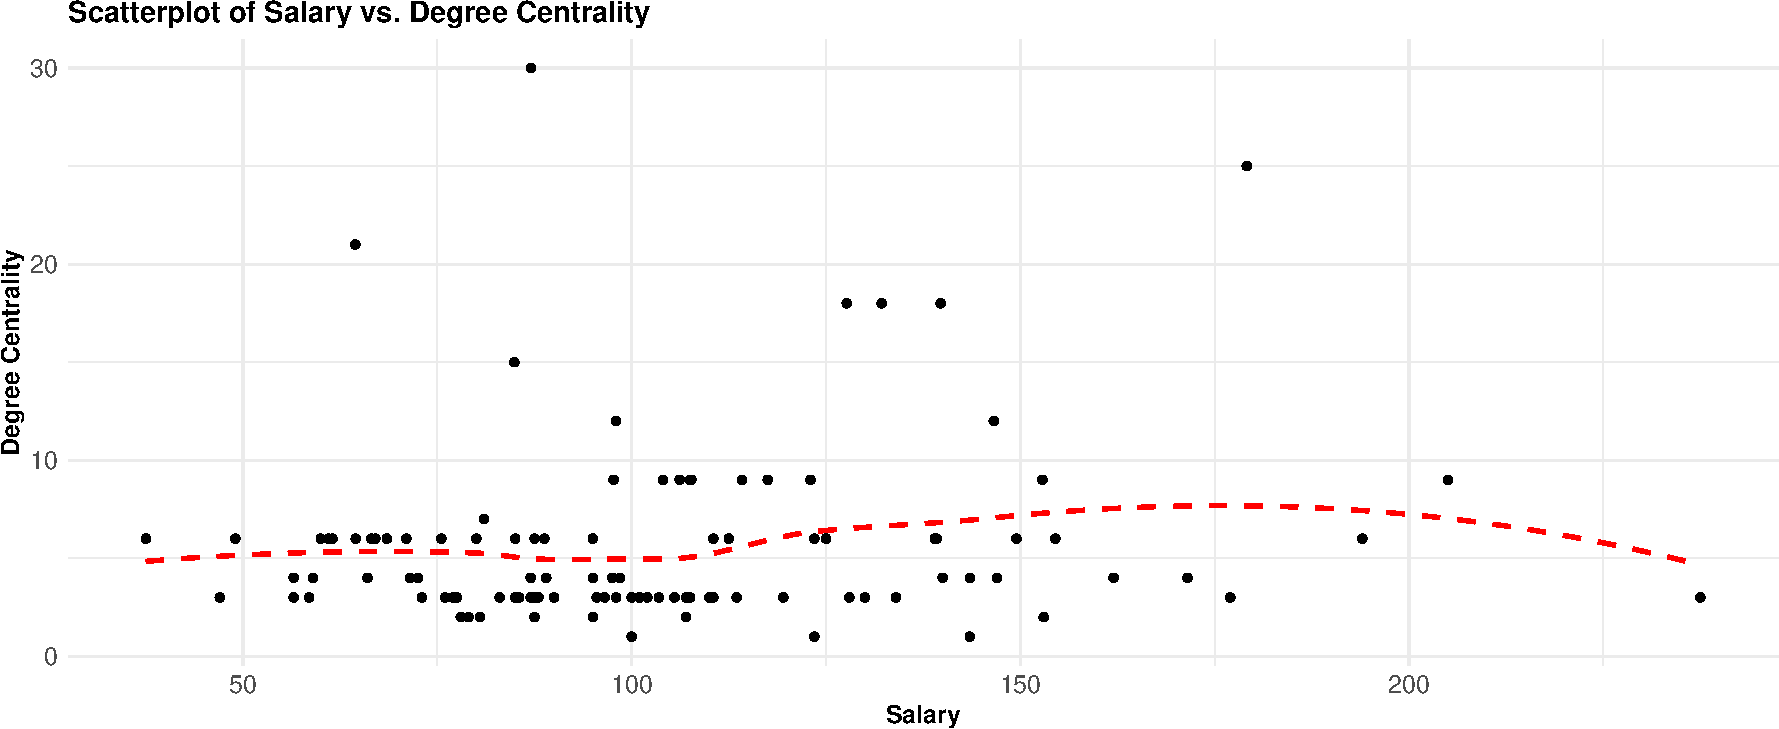
\includegraphics[keepaspectratio]{DataScience_files/figure-latex/unnamed-chunk-24-1.pdf}}
Die rote Linie zeigt einen flachen Trend ohne starke Korrelation in
diesem Scatterplot zwischen Gehalt und Degree Centrality.

Der weitgehend flache Verlauf der Trendlinie lässt den Schluss zu, dass
kein klarer Zusammenhang zwischen der Degree Centrality und den
Gehältern besteht. Dies könnte implizieren, dass die Anzahl direkter
Wettbewerber ( Degree Centrality) für sich genommen keinen signifikanten
Einfluss auf das Gehaltsniveau eines Unternehmens ausübt.

Ein kleiner Anstieg des Gehalts ist insbesondere im Bereich zwischen 100
und 150 zu verzeichnen, was darauf hindeutet, dass Unternehmen mit
mittlerem Gehaltsniveau tendenziell mehr direkte Wettbewerber haben.
Diese Entwicklung lässt sich dadurch erklären, dass Unternehmen mit
mittleren Gehaltsniveaus in stärker besetzten Märkten tätig sind, in
denen eine größere Anzahl an Unternehmen um Talente konkurriert.

Die meisten Werte der Degree Centrality sind relativ niedrig, was darauf
hindeutet, dass eine Vielzahl von Unternehmen lediglich eine geringe
Anzahl direkter Wettbewerber aufweist. Einige Unternehmen mit hoher
Degree Centrality und niedrigen bis mittleren Gehältern heben sich
jedoch von der Gesamtheit ab. Es ist möglich, dass diese Unternehmen in
stark umkämpften Märkten tätig sind, jedoch nicht über die
erforderlichen Ressourcen verfügen, um hohe Gehälter zu offerieren.

Ein Vergleich der Degree Centrality mit der Betweenness Centrality
zeigt, dass die Degree Centrality einen geringeren Einfluss auf das
Gehalt zu haben scheint. Dies lässt den Schluss zu, dass nicht die
Anzahl der direkten Wettbewerber, sondern die Position eines
Unternehmens als strategischer Vermittler im Netzwerk (Betweenness)
einflussreicher für die Höhe des Gehalts ist.

\subsubsection{Eigenvector-Zentralität}\label{eigenvector-zentralituxe4t}

Unternehmen mit hoher Eigenvector Centrality stehen nicht nur in
Konkurrenz zu einer Vielzahl von Unternehmen, sondern insbesondere zu
besonders einflussreichen Wettbewerbern im Netzwerk.

Unternehmen mit hoher Eigenvector Centrality könnten in der Konsequenz
wettbewerbsfähige Gehälter anbieten müssen, um sich im Wettbewerb mit
zentralen und attraktiven Arbeitgebern zu behaupten. Folglich sind auch
die umliegenden Firmen gezwungen, ihre Angebote anzupassen, um für die
Talente am Arbeitsmarkt attraktiv zu bleiben. Es besteht die
Möglichkeit, dass diese Unternehmen die Gehälter für spezifische,
wettbewerbsrelevante Rollen erhöhen, um den Marktstandards und den
Anforderungen eines zentralen Wettbewerbsnetzwerks gerecht zu werden.

\begin{Shaded}
\begin{Highlighting}[]
\CommentTok{\# Berechne die Eigenvector{-}Centrality und sortiere sie absteigend}
\NormalTok{top\_eigenvector }\OtherTok{\textless{}{-}} \FunctionTok{head}\NormalTok{(}\FunctionTok{sort}\NormalTok{(eigenvector\_centrality}\SpecialCharTok{$}\NormalTok{vector, }\AttributeTok{decreasing =} \ConstantTok{TRUE}\NormalTok{), }\DecValTok{5}\NormalTok{)}

\CommentTok{\# Erstelle ein DataFrame mit den Namen der Unternehmen und ihrer Eigenvector{-}Centrality}
\NormalTok{top\_eigenvector\_df }\OtherTok{\textless{}{-}} \FunctionTok{data.frame}\NormalTok{(}
  \AttributeTok{Company =} \FunctionTok{names}\NormalTok{(top\_eigenvector),}
  \AttributeTok{Eigenvector =} \FunctionTok{as.numeric}\NormalTok{(top\_eigenvector),}
  \AttributeTok{stringsAsFactors =} \ConstantTok{FALSE}
\NormalTok{)}

\CommentTok{\# Erstelle die Tabelle und zentriere sie links}
\FunctionTok{kable}\NormalTok{(top\_eigenvector\_df, }\AttributeTok{format =} \StringTok{"latex"}\NormalTok{, }\AttributeTok{booktabs =} \ConstantTok{TRUE}\NormalTok{, }\AttributeTok{align =} \StringTok{"l"}\NormalTok{) }\SpecialCharTok{\%\textgreater{}\%}
  \FunctionTok{kable\_styling}\NormalTok{(}\AttributeTok{latex\_options =} \FunctionTok{c}\NormalTok{(}\StringTok{"striped"}\NormalTok{, }\StringTok{"hold\_position"}\NormalTok{), }\AttributeTok{position =} \StringTok{"left"}\NormalTok{)}
\end{Highlighting}
\end{Shaded}

\begin{tabular}{ll}
\toprule
Company & Eigenvector\\
\midrule
\cellcolor{gray!10}{PNNL} & \cellcolor{gray!10}{1.0000000}\\
National Renewable Energy Lab & 0.5887841\\
\cellcolor{gray!10}{Oak Ridge National Laboratory} & \cellcolor{gray!10}{0.5887841}\\
Los Alamos National Laboratory & 0.5887841\\
\cellcolor{gray!10}{Pacific Northwest National Laboratory} & \cellcolor{gray!10}{0.2000000}\\
\bottomrule
\end{tabular}

\(\\\)

\begin{Shaded}
\begin{Highlighting}[]
\CommentTok{\# Berechne die Eigenvector{-}Centrality und sortiere sie absteigend}
\NormalTok{eigenvector\_centrality }\OtherTok{\textless{}{-}} \FunctionTok{evcent}\NormalTok{(g\_competitors\_zentralität, }\AttributeTok{directed =} \ConstantTok{FALSE}\NormalTok{)}\SpecialCharTok{$}\NormalTok{vector}

\CommentTok{\# Zusammenhang zwischen durchschnittliches Gehalt und Eigenvector{-}Zentralität}
\NormalTok{salary\_eigenvector }\OtherTok{\textless{}{-}} \FunctionTok{data.frame}\NormalTok{(}
  \AttributeTok{Salary =}\NormalTok{ salary\_data}\SpecialCharTok{$}\NormalTok{AverageSalary,}
  \AttributeTok{Eigenvector =}\NormalTok{ eigenvector\_centrality[}
    \FunctionTok{match}\NormalTok{(salary\_data}\SpecialCharTok{$}\StringTok{\textasciigrave{}}\AttributeTok{Company Name}\StringTok{\textasciigrave{}}\NormalTok{, }\FunctionTok{names}\NormalTok{(eigenvector\_centrality))}
\NormalTok{  ]}
\NormalTok{)}

\CommentTok{\# Entferne NA{-}Werte, die durch fehlende Übereinstimmungen entstehen könnten}
\NormalTok{salary\_eigenvector }\OtherTok{\textless{}{-}} \FunctionTok{na.omit}\NormalTok{(salary\_eigenvector)}

\CommentTok{\# Scatterplot mit roter, gestrichelter Trendlinie}
\FunctionTok{ggplot}\NormalTok{(salary\_eigenvector, }\FunctionTok{aes}\NormalTok{(}\AttributeTok{x =}\NormalTok{ Salary, }\AttributeTok{y =}\NormalTok{ Eigenvector)) }\SpecialCharTok{+}
  \FunctionTok{geom\_point}\NormalTok{() }\SpecialCharTok{+}
  \FunctionTok{geom\_smooth}\NormalTok{(}\AttributeTok{method =} \StringTok{"loess"}\NormalTok{, }\AttributeTok{se =} \ConstantTok{FALSE}\NormalTok{, }\AttributeTok{color =} \StringTok{"red"}\NormalTok{, }\AttributeTok{linetype =} \StringTok{"dashed"}\NormalTok{) }\SpecialCharTok{+}
  \FunctionTok{labs}\NormalTok{(}\AttributeTok{title =} \StringTok{"Scatterplot of Salary vs. Eigenvector Centrality"}\NormalTok{,}
       \AttributeTok{x =} \StringTok{"Salary"}\NormalTok{, }\AttributeTok{y =} \StringTok{"Eigenvector Centrality"}\NormalTok{) }\SpecialCharTok{+}
  \FunctionTok{theme\_minimal}\NormalTok{() }\SpecialCharTok{+}
  \FunctionTok{theme}\NormalTok{(}
    \AttributeTok{plot.title =} \FunctionTok{element\_text}\NormalTok{(}\AttributeTok{size =} \DecValTok{14}\NormalTok{, }\AttributeTok{face =} \StringTok{"bold"}\NormalTok{),}
    \AttributeTok{axis.title =} \FunctionTok{element\_text}\NormalTok{(}\AttributeTok{size =} \DecValTok{12}\NormalTok{, }\AttributeTok{face =} \StringTok{"bold"}\NormalTok{),}
    \AttributeTok{axis.text =} \FunctionTok{element\_text}\NormalTok{(}\AttributeTok{size =} \DecValTok{12}\NormalTok{)}
\NormalTok{  )}
\end{Highlighting}
\end{Shaded}

\begin{verbatim}
## `geom_smooth()` using formula = 'y ~ x'
\end{verbatim}

\pandocbounded{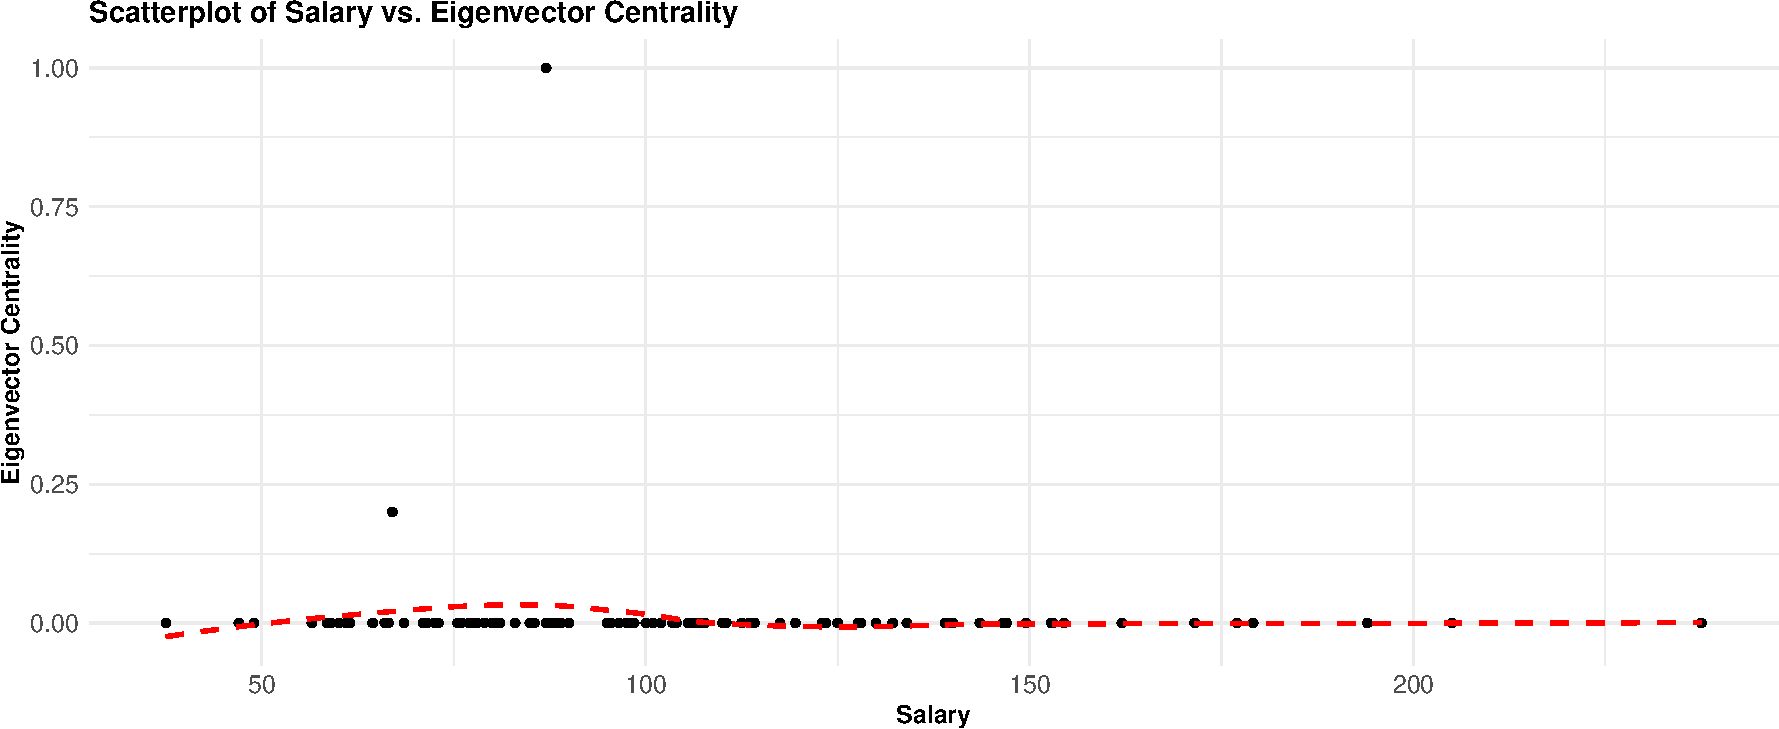
\includegraphics[keepaspectratio]{DataScience_files/figure-latex/unnamed-chunk-26-1.pdf}}
Auch im Scatterplot zwischen Gehalt und Eigenvector Centrality lässt
sich ein weitgehend flacher Trend beobachten, wie die rote Linie
veranschaulicht. Der Eigenvector Centrality-Index misst die Intensität
der Verbindungen zwischen einem Unternehmen und anderen, stark
vernetzten Unternehmen.

Die rote Linie verbleibt nahe dem Nullpunkt, was darauf hindeutet, dass
die Eigenvector Centrality keine eindeutige Korrelation mit dem Gehalt
aufweist. Diese Erkenntnis lässt den Schluss zu, dass Unternehmen, die
mit anderen stark vernetzten Firmen assoziiert sind, nicht zwangsläufig
höhere Gehälter zahlen.

Es lassen sich zwei Ausreißer identifizieren, die eine
überdurchschnittlich hohe Eigenvector-Centrality-Wertigkeit aufweisen,
obwohl sie vergleichsweise niedrige Gehälter zahlen. Es besteht die
Möglichkeit, dass diese Unternehmen in hohem Maße mit anderen gut
vernetzten Firmen verbunden sind, jedoch dennoch niedrigere Gehälter
zahlen. Dies lässt den Schluss zu, dass die zentrale Vernetzung der
Unternehmen im Wettbewerbsnetzwerk nicht ausreicht, um höhere Gehälter
zu rechtfertigen, oder dass sie in einem stark vernetzten, aber niedrig
bezahlten Segment tätig sind.

Die Analyse der Gehälter in Unternehmen mit hohen Vergütungen zeigt,
dass diese sehr niedrige Werte in der Eigenvector-Centrality aufweisen.
Dies lässt den Schluss zu, dass hohe Gehälter eher bei Unternehmen
vorkommen, die weniger stark an andere hoch vernetzte Firmen im Netzwerk
gebunden sind. Diese Unternehmen könnten eine besondere Marktstellung
oder Spezialisierung aufweisen, welche ihnen erlaubt, hohe Gehälter zu
zahlen, ohne auf enge Verbindungen zu anderen zentralen Unternehmen
angewiesen zu sein.

\subsection{Cluster-Analyse}\label{cluster-analyse}

Die Anwendung von Community-Detection-Methoden, wie beispielsweise
Louvain oder Walktrap, ermöglicht die Identifikation von Clustern von
Unternehmen, die sich durch einen besonders engen Wettbewerb
auszeichnen.

Im Rahmen der Klassifizierung und Visualisierung erfolgt eine farbliche
Markierung der identifizierten Cluster im Netzwerk, um eine bessere
Übersicht über die Wettbewerbsgruppen zu gewinnen.

Im Rahmen der Untersuchung wird ermittelt, ob Cluster existieren, in
denen besonders hohe oder niedrige Gehälter überwiegen, und ob diese
Cluster eine gemeinsame Markt- oder Branchenstruktur aufweisen.

\subsubsection{Clustering
Identifikation}\label{clustering-identifikation}

\begin{Shaded}
\begin{Highlighting}[]
\CommentTok{\# Louvain Community Detection}
\NormalTok{louvain\_community }\OtherTok{\textless{}{-}} \FunctionTok{cluster\_louvain}\NormalTok{(g\_direct\_competitors, }\AttributeTok{resolution =} \FloatTok{0.1}\NormalTok{)}

\CommentTok{\# Walktrap Community Detection}
\NormalTok{walktrap\_community }\OtherTok{\textless{}{-}} \FunctionTok{cluster\_walktrap}\NormalTok{(g\_direct\_competitors, }\AttributeTok{steps =} \DecValTok{2}\NormalTok{)}

\CommentTok{\# Wähle Louvain als Community{-}Detection{-}Methode}
\NormalTok{communities }\OtherTok{\textless{}{-}}\NormalTok{ louvain\_community}


\CommentTok{\# Füge die Community{-}Informationen zu den Knoten des Graphen hinzu}
\FunctionTok{V}\NormalTok{(g\_direct\_competitors)}\SpecialCharTok{$}\NormalTok{community }\OtherTok{\textless{}{-}} \FunctionTok{membership}\NormalTok{(communities)}

\CommentTok{\# Erstelle eine Farbpalette für die Communities}
\NormalTok{num\_communities }\OtherTok{\textless{}{-}} \FunctionTok{length}\NormalTok{(}\FunctionTok{unique}\NormalTok{(}\FunctionTok{V}\NormalTok{(g\_direct\_competitors)}\SpecialCharTok{$}\NormalTok{community))}
\ControlFlowTok{if}\NormalTok{ (num\_communities }\SpecialCharTok{\textgreater{}} \DecValTok{12}\NormalTok{) \{}
\NormalTok{  community\_colors }\OtherTok{\textless{}{-}} \FunctionTok{colorRampPalette}\NormalTok{(}\FunctionTok{brewer.pal}\NormalTok{(}\DecValTok{12}\NormalTok{, }\StringTok{"Set3"}\NormalTok{))(num\_communities)}
\NormalTok{\} }\ControlFlowTok{else}\NormalTok{ \{}
\NormalTok{  community\_colors }\OtherTok{\textless{}{-}} \FunctionTok{brewer.pal}\NormalTok{(num\_communities, }\StringTok{"Set3"}\NormalTok{)}
\NormalTok{\}}

\CommentTok{\# Weise die Farben den Knoten basierend auf ihrer Community zu}
\FunctionTok{V}\NormalTok{(g\_direct\_competitors)}\SpecialCharTok{$}\NormalTok{color }\OtherTok{\textless{}{-}}\NormalTok{ community\_colors[}\FunctionTok{V}\NormalTok{(g\_direct\_competitors)}\SpecialCharTok{$}\NormalTok{community]}

\CommentTok{\# Visualisiere das Netzwerk mit den Community{-}Farben}
\FunctionTok{plot}\NormalTok{(g\_direct\_competitors, }\AttributeTok{vertex.label =} \ConstantTok{NA}\NormalTok{,}
     \AttributeTok{vertex.size =} \DecValTok{3}\NormalTok{,  }\CommentTok{\# Kleinere Knoten}
     \AttributeTok{edge.width =} \DecValTok{1} \SpecialCharTok{*} \FunctionTok{E}\NormalTok{(g\_direct\_competitors)}\SpecialCharTok{$}\NormalTok{weight, }\CommentTok{\# Reduzierte Gewichtung der Kanten}
     \AttributeTok{edge.arrow.size =} \DecValTok{1}\NormalTok{,}
     \AttributeTok{layout =}\NormalTok{ layout\_with\_fr,}
\NormalTok{)}
\FunctionTok{title}\NormalTok{(}\AttributeTok{main =} \StringTok{"Unternehmensnetzwerk mit Community{-}Detection (Louvain)"}\NormalTok{, }\AttributeTok{cex.main =} \DecValTok{2}\NormalTok{)}
\end{Highlighting}
\end{Shaded}

\pandocbounded{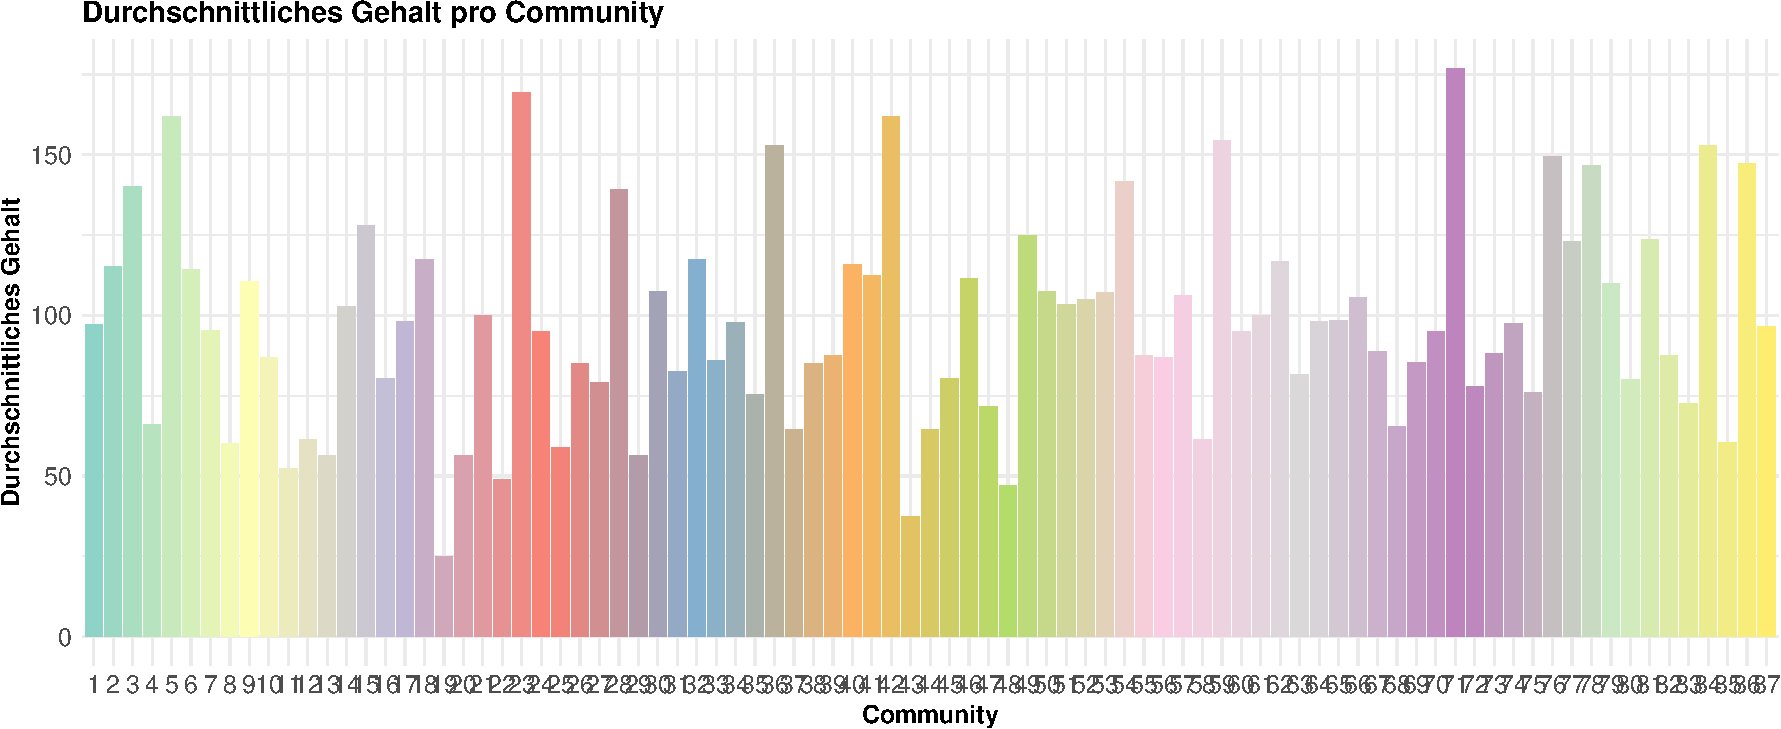
\includegraphics[keepaspectratio]{DataScience_files/figure-latex/unnamed-chunk-27-1.pdf}}

\begin{Shaded}
\begin{Highlighting}[]
\CommentTok{\# Berechne die Größe der Cluster}
\NormalTok{cluster\_sizes }\OtherTok{\textless{}{-}} \FunctionTok{table}\NormalTok{(}\FunctionTok{membership}\NormalTok{(communities))}

\CommentTok{\# Sortiere die Cluster nach Größe absteigend}
\NormalTok{sorted\_clusters }\OtherTok{\textless{}{-}} \FunctionTok{sort}\NormalTok{(cluster\_sizes, }\AttributeTok{decreasing =} \ConstantTok{TRUE}\NormalTok{)}

\CommentTok{\# Erstelle ein DataFrame mit den Cluster{-}Informationen}
\NormalTok{cluster\_info }\OtherTok{\textless{}{-}} \FunctionTok{data.frame}\NormalTok{(}
  \AttributeTok{Cluster =} \FunctionTok{names}\NormalTok{(sorted\_clusters),}
  \AttributeTok{Size =} \FunctionTok{as.numeric}\NormalTok{(sorted\_clusters),}
  \AttributeTok{stringsAsFactors =} \ConstantTok{FALSE}
\NormalTok{)}

\CommentTok{\# Ausgeben wie viele Cluster es gibt}
\FunctionTok{print}\NormalTok{(}\FunctionTok{paste}\NormalTok{(}\StringTok{"Anzahl der Cluster:"}\NormalTok{, }\FunctionTok{length}\NormalTok{(cluster\_info}\SpecialCharTok{$}\NormalTok{Cluster)))}
\end{Highlighting}
\end{Shaded}

\begin{verbatim}
## [1] "Anzahl der Cluster: 79"
\end{verbatim}

\begin{Shaded}
\begin{Highlighting}[]
\CommentTok{\# Auswahl der 7 größten Cluster}
\NormalTok{top\_clusters }\OtherTok{\textless{}{-}} \FunctionTok{head}\NormalTok{(sorted\_clusters, }\DecValTok{7}\NormalTok{)}

\CommentTok{\# Ausgabe der 7 größten Cluster}
\NormalTok{top\_clusters\_df }\OtherTok{\textless{}{-}} \FunctionTok{data.frame}\NormalTok{(}
\AttributeTok{Cluster =} \FunctionTok{names}\NormalTok{(top\_clusters),}
\AttributeTok{Size =} \FunctionTok{as.numeric}\NormalTok{(top\_clusters),}
\AttributeTok{stringsAsFactors =} \ConstantTok{FALSE}
\NormalTok{)}

\CommentTok{\# Erstelle die Tabelle und zentriere sie links}
\FunctionTok{kable}\NormalTok{(top\_clusters\_df, }\AttributeTok{format =} \StringTok{"latex"}\NormalTok{, }\AttributeTok{booktabs =} \ConstantTok{TRUE}\NormalTok{, }\AttributeTok{align =} \StringTok{"l"}\NormalTok{) }\SpecialCharTok{\%\textgreater{}\%}
  \FunctionTok{kable\_styling}\NormalTok{(}\AttributeTok{latex\_options =} \FunctionTok{c}\NormalTok{(}\StringTok{"striped"}\NormalTok{, }\StringTok{"hold\_position"}\NormalTok{),}
                \AttributeTok{position =} \StringTok{"left"}\NormalTok{)}
\end{Highlighting}
\end{Shaded}

\begin{tabular}{ll}
\toprule
Cluster & Size\\
\midrule
\cellcolor{gray!10}{1} & \cellcolor{gray!10}{44}\\
8 & 13\\
\cellcolor{gray!10}{35} & \cellcolor{gray!10}{9}\\
5 & 8\\
\cellcolor{gray!10}{15} & \cellcolor{gray!10}{8}\\
\addlinespace
19 & 7\\
\cellcolor{gray!10}{12} & \cellcolor{gray!10}{6}\\
\bottomrule
\end{tabular}

\(\\\) Da das Netzwerk sehr fragmentiert ist, werden im folgenden
Schritt bloß die 7 größten Cluster betrachtet. \(\\\)

\begin{Shaded}
\begin{Highlighting}[]
\CommentTok{\# Berechne die Größe der Cluster}
\NormalTok{cluster\_sizes }\OtherTok{\textless{}{-}} \FunctionTok{table}\NormalTok{(}\FunctionTok{membership}\NormalTok{(communities))}

\CommentTok{\# Sortiere die Cluster nach Größe absteigend}
\NormalTok{sorted\_clusters }\OtherTok{\textless{}{-}} \FunctionTok{sort}\NormalTok{(cluster\_sizes, }\AttributeTok{decreasing =} \ConstantTok{TRUE}\NormalTok{)}

\CommentTok{\# Auswahl der 7 größten Cluster}
\NormalTok{top\_clusters }\OtherTok{\textless{}{-}} \FunctionTok{head}\NormalTok{(sorted\_clusters, }\DecValTok{7}\NormalTok{)}

\CommentTok{\# Erstelle eine Farbpalette für die Top 7 Cluster}
\NormalTok{top\_cluster\_ids }\OtherTok{\textless{}{-}} \FunctionTok{names}\NormalTok{(top\_clusters)}
\NormalTok{num\_top\_clusters }\OtherTok{\textless{}{-}} \FunctionTok{length}\NormalTok{(top\_cluster\_ids)}
\NormalTok{top\_cluster\_colors }\OtherTok{\textless{}{-}} \FunctionTok{brewer.pal}\NormalTok{(}\FunctionTok{min}\NormalTok{(num\_top\_clusters, }\DecValTok{12}\NormalTok{), }\StringTok{"Set3"}\NormalTok{)}

\CommentTok{\# Weise die Farben den Knoten basierend auf ihrer Zugehörigkeit zu den Top 7 Clustern zu}
\FunctionTok{V}\NormalTok{(g\_direct\_competitors)}\SpecialCharTok{$}\NormalTok{color }\OtherTok{\textless{}{-}} \FunctionTok{ifelse}\NormalTok{(}
  \FunctionTok{V}\NormalTok{(g\_direct\_competitors)}\SpecialCharTok{$}\NormalTok{community }\SpecialCharTok{\%in\%}\NormalTok{ top\_cluster\_ids,}
\NormalTok{  top\_cluster\_colors[}
    \FunctionTok{match}\NormalTok{(}\FunctionTok{V}\NormalTok{(g\_direct\_competitors)}\SpecialCharTok{$}\NormalTok{community, top\_cluster\_ids)}
\NormalTok{  ],}
  \StringTok{"grey"}
\NormalTok{)}

\CommentTok{\# Visualisiere das Netzwerk mit den Community{-}Farben}
\FunctionTok{plot}\NormalTok{(g\_direct\_competitors, }\AttributeTok{vertex.label =} \ConstantTok{NA}\NormalTok{,}
     \AttributeTok{vertex.size =} \DecValTok{3}\NormalTok{,  }\CommentTok{\# Kleinere Knoten}
     \AttributeTok{edge.width =} \DecValTok{1} \SpecialCharTok{*} \FunctionTok{E}\NormalTok{(g\_direct\_competitors)}\SpecialCharTok{$}\NormalTok{weight,  }\CommentTok{\# Reduzierte Gewichtung}
     \AttributeTok{edge.arrow.size =} \DecValTok{1}\NormalTok{,}
     \AttributeTok{layout =}\NormalTok{ layout\_with\_fr}
\NormalTok{)}
\FunctionTok{title}\NormalTok{(}\AttributeTok{main =} \StringTok{"Die 7 größten Cluster im Unternehmensnetzwerk"}\NormalTok{, }\AttributeTok{cex.main =} \DecValTok{2}\NormalTok{)}

\CommentTok{\# Legende für Cluster{-}Farben}
\FunctionTok{legend}\NormalTok{(}\StringTok{"topright"}\NormalTok{, }\AttributeTok{legend =} \FunctionTok{c}\NormalTok{(top\_cluster\_ids, }\StringTok{"Andere"}\NormalTok{),}
       \AttributeTok{fill =} \FunctionTok{c}\NormalTok{(top\_cluster\_colors, }\StringTok{"grey"}\NormalTok{))}
\end{Highlighting}
\end{Shaded}

\pandocbounded{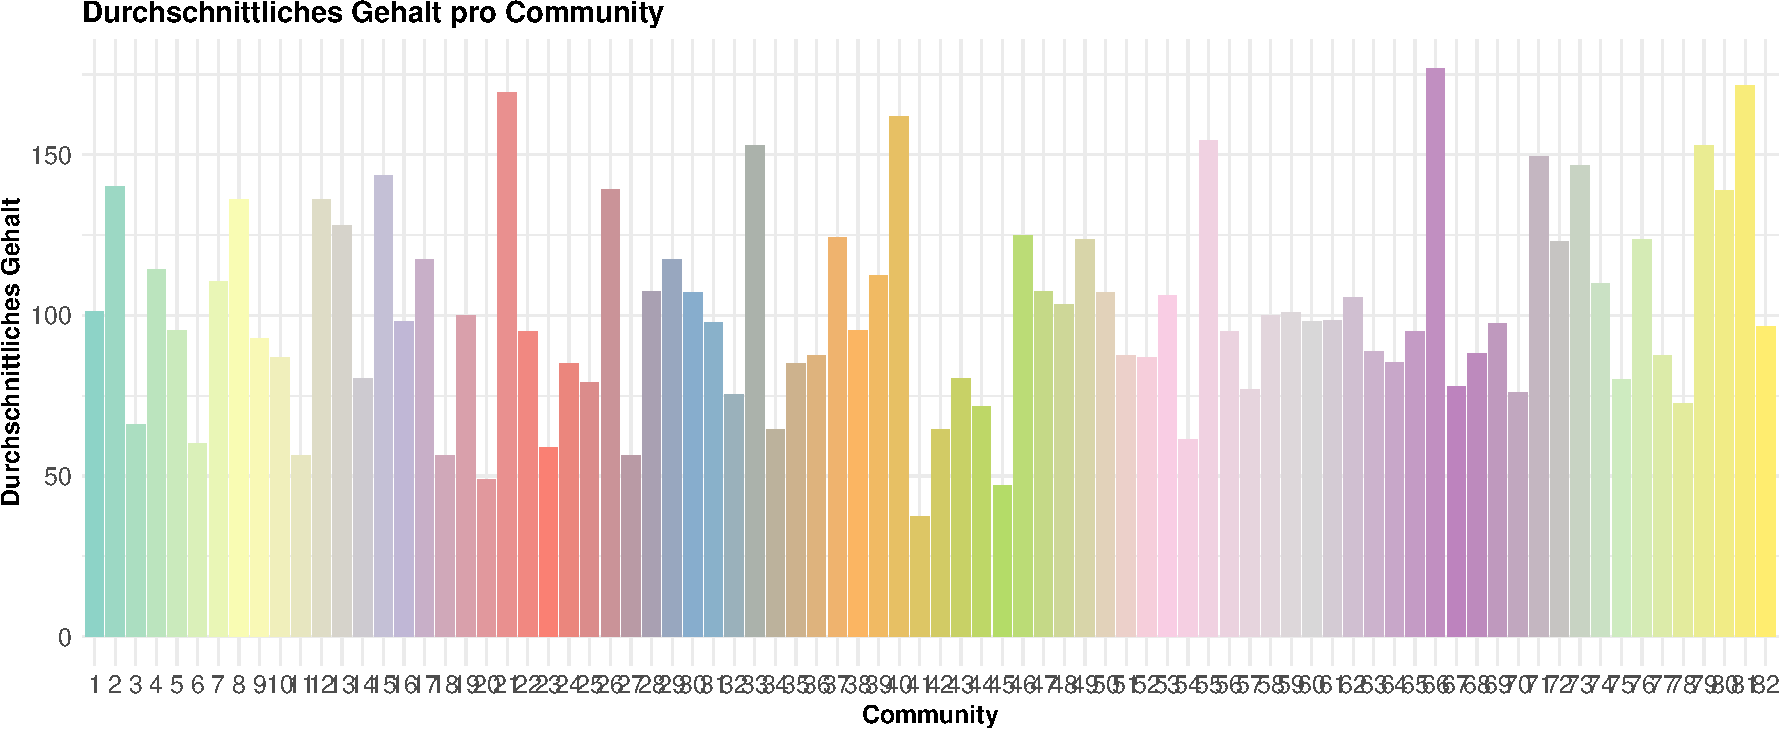
\includegraphics[keepaspectratio]{DataScience_files/figure-latex/unnamed-chunk-30-1.pdf}}

\subsubsection{Gehaltsunterschiede zwischen den
Clustern}\label{gehaltsunterschiede-zwischen-den-clustern}

Der Boxplot zeigt die Verteilung der Durchschnittsgehälter in den Top 7
Clustern.

\begin{Shaded}
\begin{Highlighting}[]
\CommentTok{\# Nimmt die top\_cluster und fügt sie in ein Dataframe}
\NormalTok{top\_clusters\_df }\OtherTok{\textless{}{-}} \FunctionTok{data.frame}\NormalTok{(}
  \AttributeTok{Cluster =} \FunctionTok{names}\NormalTok{(top\_clusters),}
  \AttributeTok{Size =} \FunctionTok{as.numeric}\NormalTok{(top\_clusters),}
  \AttributeTok{stringsAsFactors =} \ConstantTok{FALSE}
\NormalTok{)}

\CommentTok{\# Erstelle eine leere Liste für die Durchschnittsgehälter der Cluster}
\NormalTok{cluster\_salaries }\OtherTok{\textless{}{-}} \FunctionTok{list}\NormalTok{()}

\CommentTok{\# Berechne die Durchschnittsgehälter für jeden Cluster}
\ControlFlowTok{for}\NormalTok{ (cluster\_id }\ControlFlowTok{in} \FunctionTok{names}\NormalTok{(top\_clusters)) \{}
\NormalTok{  cluster\_members }\OtherTok{\textless{}{-}} \FunctionTok{V}\NormalTok{(g\_direct\_competitors)}\SpecialCharTok{$}\NormalTok{name[}
    \FunctionTok{V}\NormalTok{(g\_direct\_competitors)}\SpecialCharTok{$}\NormalTok{community }\SpecialCharTok{==}\NormalTok{ cluster\_id}
\NormalTok{  ]}
\NormalTok{  cluster\_salaries[[cluster\_id]] }\OtherTok{\textless{}{-}}\NormalTok{ salary\_data}\SpecialCharTok{$}\NormalTok{AverageSalary[}
\NormalTok{    salary\_data}\SpecialCharTok{$}\StringTok{\textasciigrave{}}\AttributeTok{Company Name}\StringTok{\textasciigrave{}} \SpecialCharTok{\%in\%}\NormalTok{ cluster\_members}
\NormalTok{  ]}
\NormalTok{\}}

\CommentTok{\# Erstelle ein DataFrame mit den Durchschnittsgehältern der Cluster}
\NormalTok{cluster\_salaries\_df }\OtherTok{\textless{}{-}} \FunctionTok{data.frame}\NormalTok{(}
  \AttributeTok{Cluster =} \FunctionTok{rep}\NormalTok{(}\FunctionTok{names}\NormalTok{(top\_clusters), }\FunctionTok{sapply}\NormalTok{(cluster\_salaries, length)),}
  \AttributeTok{Salary =} \FunctionTok{unlist}\NormalTok{(cluster\_salaries),}
  \AttributeTok{stringsAsFactors =} \ConstantTok{FALSE}
\NormalTok{)}

\CommentTok{\# Erstelle ein Boxplot der Gehälter nach Cluster}
\FunctionTok{ggplot}\NormalTok{(cluster\_salaries\_df, }\FunctionTok{aes}\NormalTok{(}\AttributeTok{x =}\NormalTok{ Cluster, }\AttributeTok{y =}\NormalTok{ Salary, }\AttributeTok{fill =}\NormalTok{ Cluster)) }\SpecialCharTok{+}
  \FunctionTok{geom\_boxplot}\NormalTok{() }\SpecialCharTok{+}
  \FunctionTok{labs}\NormalTok{(}\AttributeTok{title =} \StringTok{"Boxplot der Durchschnittsgehälter nach Cluster"}\NormalTok{,}
       \AttributeTok{x =} \StringTok{"Cluster"}\NormalTok{, }\AttributeTok{y =} \StringTok{"Average Salary"}\NormalTok{) }\SpecialCharTok{+}
  \FunctionTok{theme\_minimal}\NormalTok{() }\SpecialCharTok{+}
  \FunctionTok{theme}\NormalTok{(}
    \AttributeTok{plot.title =} \FunctionTok{element\_text}\NormalTok{(}\AttributeTok{size =} \DecValTok{18}\NormalTok{, }\AttributeTok{face =} \StringTok{"bold"}\NormalTok{),}
    \AttributeTok{axis.title =} \FunctionTok{element\_text}\NormalTok{(}\AttributeTok{size =} \DecValTok{14}\NormalTok{, }\AttributeTok{face =} \StringTok{"bold"}\NormalTok{),}
    \AttributeTok{axis.text =} \FunctionTok{element\_text}\NormalTok{(}\AttributeTok{size =} \DecValTok{14}\NormalTok{)}
\NormalTok{  )}
\end{Highlighting}
\end{Shaded}

\pandocbounded{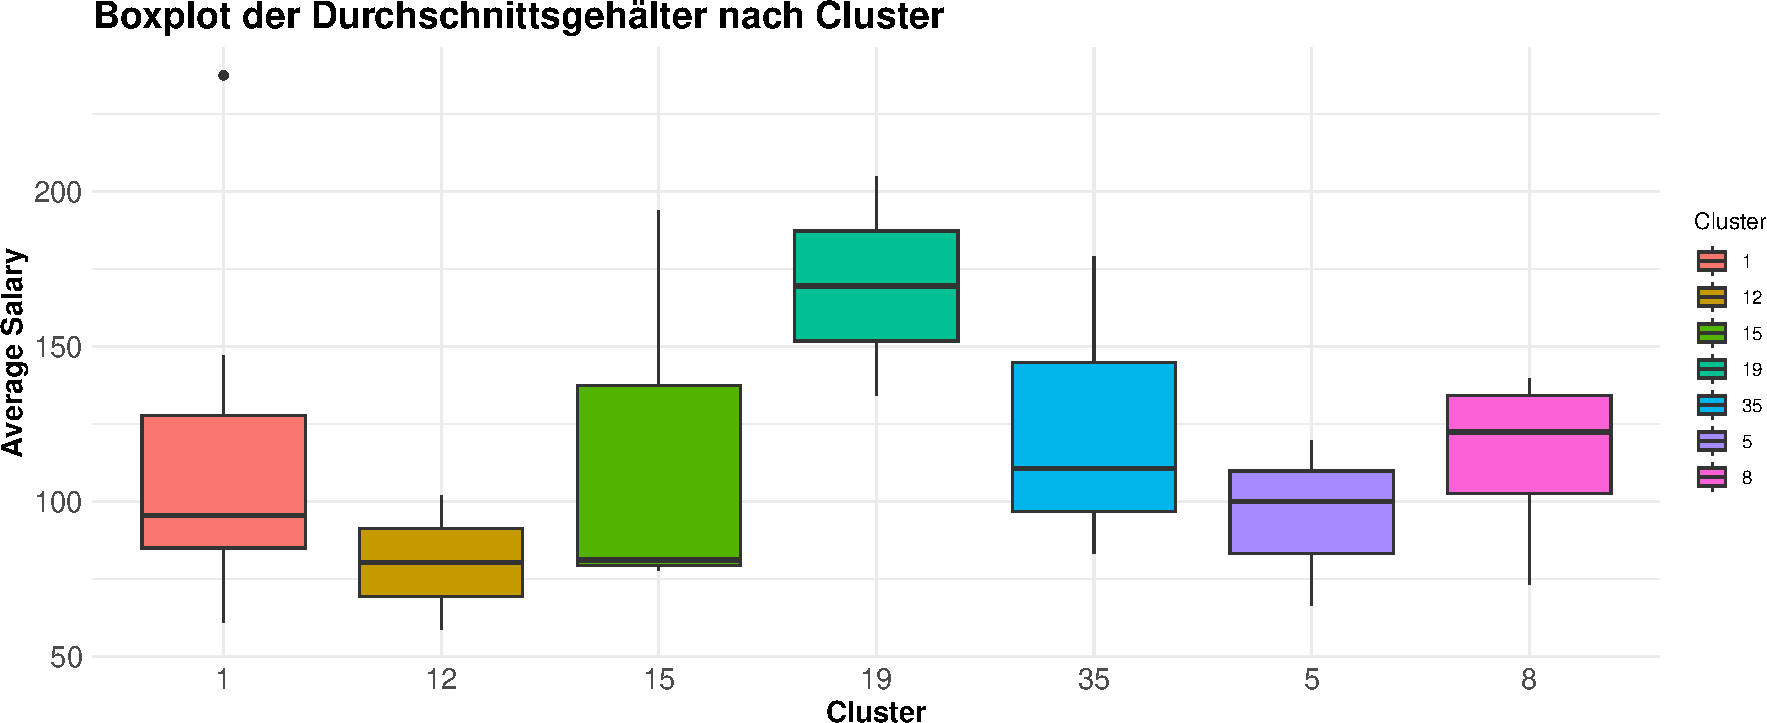
\includegraphics[keepaspectratio]{DataScience_files/figure-latex/unnamed-chunk-31-1.pdf}}
\(\\\) Die höchsten Gehälter werden in den Clustern 19 und 15 gezahlt.
Dabei weist Cluster 19 die höchsten Durchschnittsgehälter auf. Die
Gehaltsverteilung in Cluster 15 ist hingegen sehr heterogen, was darauf
hindeutet, dass in diesem Cluster sowohl hoch als auch niedrig bezahlte
Positionen vertreten sind.

Die Cluster 12 und 5 weisen die niedrigsten Durchschnittsgehälter auf.
Die Gehälter in diesen Clustern sind relativ gering und weisen zudem
eine geringe Variabilität auf. Dies könnte auf eine homogene Struktur
der Gehaltsstufen hindeuten.

Die beiden Cluster 35 und Cluster 1, lassen sich dem mittleren Bereich
zuordnen, wobei Cluster 35 eine breite Streuung aufweist. Dies lässt den
Schluss zu, dass innerhalb dieses Clusters eine signifikante Varianz
besteht, was auf eine Mischung aus verschiedenen Unternehmensarten oder
Positionen mit unterschiedlichen Gehältern hindeuten könnte.

Cluster 8 weist ebenfalls einen mittleren Gehaltsbereich auf, jedoch mit
einer geringeren Streuung als Cluster 35. Dies lässt auf eine gewisse
Homogenität in den Gehaltsstrukturen innerhalb dieses Clusters
schließen.

Die beiden Cluster mit der breitesten Streuung (15 und 35) könnten auf
heterogene Unternehmen hinweisen, die in unterschiedlichen Branchen oder
Positionen tätig sind und daher ein breiteres Gehaltsspektrum aufweisen.

Die Analyse der Gehaltsstruktur nach Cluster offenbart eine signifikante
Variation in den Gehaltsniveaus zwischen den einzelnen Clustern. Cluster
mit hoher Gehaltsstreuung lassen auf eine beträchtliche Diversität
hinsichtlich der Unternehmensgrößen und -typen schließen, während
Cluster mit geringer Streuung eine höhere Homogenität aufweisen.

\subsubsection{Branchenstruktur der
Cluster}\label{branchenstruktur-der-cluster}

Die Branchenzugehörigkeit der Unternehmen in den Top 7 Clustern wird im
folgenden Schritt untersucht, um festzustellen, ob die Cluster eine
gemeinsame Markt- oder Branchenstruktur aufweisen. \(\\\)

\begin{Shaded}
\begin{Highlighting}[]
\CommentTok{\# Erstelle eine leere Liste für die Branchen der Cluster}
\NormalTok{cluster\_industries }\OtherTok{\textless{}{-}} \FunctionTok{list}\NormalTok{()}

\CommentTok{\# Extrahiere die Branchen der Unternehmen in den Clustern}
\ControlFlowTok{for}\NormalTok{ (cluster\_id }\ControlFlowTok{in} \FunctionTok{names}\NormalTok{(top\_clusters)) \{}
\NormalTok{  cluster\_members }\OtherTok{\textless{}{-}} \FunctionTok{V}\NormalTok{(g\_direct\_competitors)}\SpecialCharTok{$}\NormalTok{name[}
    \FunctionTok{V}\NormalTok{(g\_direct\_competitors)}\SpecialCharTok{$}\NormalTok{community }\SpecialCharTok{==}\NormalTok{ cluster\_id]}
\NormalTok{  cluster\_industries[[cluster\_id]] }\OtherTok{\textless{}{-}}\NormalTok{ data}\SpecialCharTok{$}\NormalTok{Industry[}
\NormalTok{    data}\SpecialCharTok{$}\StringTok{\textasciigrave{}}\AttributeTok{Company Name}\StringTok{\textasciigrave{}} \SpecialCharTok{\%in\%}\NormalTok{ cluster\_members}
\NormalTok{  ]}
\NormalTok{\}}

\CommentTok{\# Erstelle Tabellen für jedes Cluster}
\ControlFlowTok{for}\NormalTok{ (cluster\_id }\ControlFlowTok{in} \FunctionTok{names}\NormalTok{(cluster\_industries)) \{}
  \CommentTok{\# Berechne die Anzahl der einzigartigen Branchen in jedem Cluster}
\NormalTok{  industry\_counts }\OtherTok{\textless{}{-}} \FunctionTok{as.data.frame}\NormalTok{(}\FunctionTok{table}\NormalTok{(cluster\_industries[[cluster\_id]]))}
  \FunctionTok{colnames}\NormalTok{(industry\_counts) }\OtherTok{\textless{}{-}} \FunctionTok{c}\NormalTok{(}\StringTok{"Industry"}\NormalTok{, }\StringTok{"Count"}\NormalTok{)}

  \CommentTok{\# Erstelle eine Tabelle für das aktuelle Cluster}
  \FunctionTok{cat}\NormalTok{(}\FunctionTok{paste0}\NormalTok{(}\StringTok{"**Cluster "}\NormalTok{, cluster\_id, }\StringTok{"**}\SpecialCharTok{\textbackslash{}n\textbackslash{}n}\StringTok{"}\NormalTok{))}
\NormalTok{  kable\_output }\OtherTok{\textless{}{-}} \FunctionTok{kable}\NormalTok{(industry\_counts, }\AttributeTok{format =} \StringTok{"latex"}\NormalTok{, }\AttributeTok{booktabs =} \ConstantTok{TRUE}\NormalTok{,}
                        \AttributeTok{align =} \StringTok{"l"}\NormalTok{) }\SpecialCharTok{\%\textgreater{}\%}
    \FunctionTok{kable\_styling}\NormalTok{(}\AttributeTok{latex\_options =} \FunctionTok{c}\NormalTok{(}\StringTok{"striped"}\NormalTok{, }\StringTok{"hold\_position"}\NormalTok{),}
                  \AttributeTok{position =} \StringTok{"left"}\NormalTok{)}
  \FunctionTok{print}\NormalTok{(kable\_output)}
  \FunctionTok{cat}\NormalTok{(}\StringTok{"}\SpecialCharTok{\textbackslash{}n\textbackslash{}n}\StringTok{"}\NormalTok{)}
  \FunctionTok{cat}\NormalTok{(}\StringTok{"\_\_}\SpecialCharTok{\textbackslash{}n\textbackslash{}n}\StringTok{"}\NormalTok{)}
\NormalTok{\}}
\end{Highlighting}
\end{Shaded}

\textbf{Cluster 1}

\begin{tabular}{ll}
\toprule
Industry & Count\\
\midrule
\cellcolor{gray!10}{Aerospace \& Defense} & \cellcolor{gray!10}{2}\\
Biotech \& Pharmaceuticals & 2\\
\cellcolor{gray!10}{Computer Hardware \& Software} & \cellcolor{gray!10}{2}\\
Consulting & 4\\
\cellcolor{gray!10}{Enterprise Software \& Network Solutions} & \cellcolor{gray!10}{7}\\
\addlinespace
Federal Agencies & 5\\
\cellcolor{gray!10}{IT Services} & \cellcolor{gray!10}{12}\\
\bottomrule
\end{tabular}

\_\_

\textbf{Cluster 8}

\begin{tabular}{ll}
\toprule
Industry & Count\\
\midrule
\cellcolor{gray!10}{Biotech \& Pharmaceuticals} & \cellcolor{gray!10}{14}\\
Health Care Products Manufacturing & 1\\
\bottomrule
\end{tabular}

\_\_

\textbf{Cluster 35}

\begin{tabular}{ll}
\toprule
Industry & Count\\
\midrule
\cellcolor{gray!10}{Insurance Carriers} & \cellcolor{gray!10}{10}\\
\bottomrule
\end{tabular}

\_\_

\textbf{Cluster 5}

\begin{tabular}{ll}
\toprule
Industry & Count\\
\midrule
\cellcolor{gray!10}{Health Care Services \& Hospitals} & \cellcolor{gray!10}{1}\\
Insurance Carriers & 3\\
\bottomrule
\end{tabular}

\_\_

\textbf{Cluster 15}

\begin{tabular}{ll}
\toprule
Industry & Count\\
\midrule
\cellcolor{gray!10}{Enterprise Software \& Network Solutions} & \cellcolor{gray!10}{2}\\
Industrial Manufacturing & 3\\
\bottomrule
\end{tabular}

\_\_

\textbf{Cluster 19}

\begin{tabular}{ll}
\toprule
Industry & Count\\
\midrule
\cellcolor{gray!10}{Advertising \& Marketing} & \cellcolor{gray!10}{1}\\
Information Technology & 3\\
\bottomrule
\end{tabular}

\_\_

\textbf{Cluster 12}

\begin{tabular}{ll}
\toprule
Industry & Count\\
\midrule
\cellcolor{gray!10}{Insurance Carriers} & \cellcolor{gray!10}{2}\\
\bottomrule
\end{tabular}

\_\_

\subsubsection{Errechnung der durchschnittlichen Gehälter pro
Branche}\label{errechnung-der-durchschnittlichen-gehuxe4lter-pro-branche}

Im Folgenden erfolgt eine Analyse der durchschnittlichen Gehaltsstruktur
pro Branche in den Top-7-Clustern. Ziel ist die Feststellung, ob
bestimmte Branchen tendenziell höhere oder niedrigere Gehälter anbieten.
Dazu wird auf der vorhergehenden Analyse aufgebaut, um die Vertretung
der verschiedenen Branchen in den Clustern und die spezifischen
Gehaltsstrukturen einbeziehen zu können. \(\\\)

\begin{Shaded}
\begin{Highlighting}[]
\CommentTok{\# Lade das Paket "viridis" für eine bessere Farbpalette}
\FunctionTok{library}\NormalTok{(viridis)}
\end{Highlighting}
\end{Shaded}

\begin{verbatim}
## Loading required package: viridisLite
\end{verbatim}

\begin{Shaded}
\begin{Highlighting}[]
\CommentTok{\# Erstelle eine leere Liste für die Durchschnittsgehälter pro Branche}
\NormalTok{industry\_salaries }\OtherTok{\textless{}{-}} \FunctionTok{list}\NormalTok{()}

\CommentTok{\# Extrahiere die Branchen und Gehälter der Unternehmen in den Clustern}
\ControlFlowTok{for}\NormalTok{ (cluster\_id }\ControlFlowTok{in} \FunctionTok{names}\NormalTok{(top\_clusters)) \{}
\NormalTok{  cluster\_members }\OtherTok{\textless{}{-}} \FunctionTok{V}\NormalTok{(g\_direct\_competitors)}\SpecialCharTok{$}\NormalTok{name[}
    \FunctionTok{V}\NormalTok{(g\_direct\_competitors)}\SpecialCharTok{$}\NormalTok{community }\SpecialCharTok{==}\NormalTok{ cluster\_id}
\NormalTok{  ]}
\NormalTok{  cluster\_data }\OtherTok{\textless{}{-}}\NormalTok{ data[data}\SpecialCharTok{$}\StringTok{\textasciigrave{}}\AttributeTok{Company Name}\StringTok{\textasciigrave{}} \SpecialCharTok{\%in\%}\NormalTok{ cluster\_members, ]}

  \CommentTok{\# Berechne die Durchschnittsgehälter pro Branche}
\NormalTok{  industry\_salaries[[cluster\_id]] }\OtherTok{\textless{}{-}}\NormalTok{ cluster\_data }\SpecialCharTok{\%\textgreater{}\%}
    \FunctionTok{group\_by}\NormalTok{(Industry) }\SpecialCharTok{\%\textgreater{}\%}
    \FunctionTok{summarise}\NormalTok{(}\AttributeTok{AverageSalary =} \FunctionTok{mean}\NormalTok{(}\StringTok{\textasciigrave{}}\AttributeTok{Salary Estimate}\StringTok{\textasciigrave{}}\NormalTok{, }\AttributeTok{na.rm =} \ConstantTok{TRUE}\NormalTok{)) }\SpecialCharTok{\%\textgreater{}\%}
    \FunctionTok{mutate}\NormalTok{(}\AttributeTok{Cluster =}\NormalTok{ cluster\_id) }\SpecialCharTok{\%\textgreater{}\%}
    \FunctionTok{arrange}\NormalTok{(}\FunctionTok{desc}\NormalTok{(AverageSalary))}
\NormalTok{\}}

\CommentTok{\# Kombiniere die Daten aus allen Clustern}
\NormalTok{combined\_industry\_salaries }\OtherTok{\textless{}{-}} \FunctionTok{bind\_rows}\NormalTok{(industry\_salaries)}

\CommentTok{\# Visualisiere die Durchschnittsgehälter pro Branche über alle Cluster hinweg}
\FunctionTok{ggplot}\NormalTok{(combined\_industry\_salaries,}
       \FunctionTok{aes}\NormalTok{(}\AttributeTok{x =} \FunctionTok{reorder}\NormalTok{(Industry, }\SpecialCharTok{{-}}\NormalTok{AverageSalary),}
           \AttributeTok{y =}\NormalTok{ AverageSalary,}
           \AttributeTok{fill =}\NormalTok{ Cluster)) }\SpecialCharTok{+}
  \FunctionTok{geom\_bar}\NormalTok{(}\AttributeTok{stat =} \StringTok{"identity"}\NormalTok{, }\AttributeTok{position =} \StringTok{"dodge"}\NormalTok{) }\SpecialCharTok{+}
  \FunctionTok{scale\_fill\_viridis\_d}\NormalTok{() }\SpecialCharTok{+}
  \FunctionTok{labs}\NormalTok{(}\AttributeTok{title =} \StringTok{"Durchschnittsgehälter nach Branche über alle Cluster hinweg"}\NormalTok{,}
       \AttributeTok{x =} \StringTok{"Branche"}\NormalTok{, }\AttributeTok{y =} \StringTok{"Durchschnittsgehalt"}\NormalTok{) }\SpecialCharTok{+}
  \FunctionTok{theme\_minimal}\NormalTok{() }\SpecialCharTok{+}
  \FunctionTok{theme}\NormalTok{(}
    \AttributeTok{plot.title =} \FunctionTok{element\_text}\NormalTok{(}\AttributeTok{size =} \DecValTok{18}\NormalTok{, }\AttributeTok{face =} \StringTok{"bold"}\NormalTok{),}
    \AttributeTok{axis.title =} \FunctionTok{element\_text}\NormalTok{(}\AttributeTok{size =} \DecValTok{14}\NormalTok{, }\AttributeTok{face =} \StringTok{"bold"}\NormalTok{),}
    \AttributeTok{axis.text =} \FunctionTok{element\_text}\NormalTok{(}\AttributeTok{size =} \DecValTok{14}\NormalTok{),}
    \AttributeTok{axis.text.x =} \FunctionTok{element\_text}\NormalTok{(}\AttributeTok{angle =} \DecValTok{45}\NormalTok{, }\AttributeTok{hjust =} \DecValTok{1}\NormalTok{)}
\NormalTok{  ) }\SpecialCharTok{+}
  \FunctionTok{coord\_flip}\NormalTok{()  }\CommentTok{\# Optional: Drehe das Diagramm für bessere Lesbarkeit}
\end{Highlighting}
\end{Shaded}

\pandocbounded{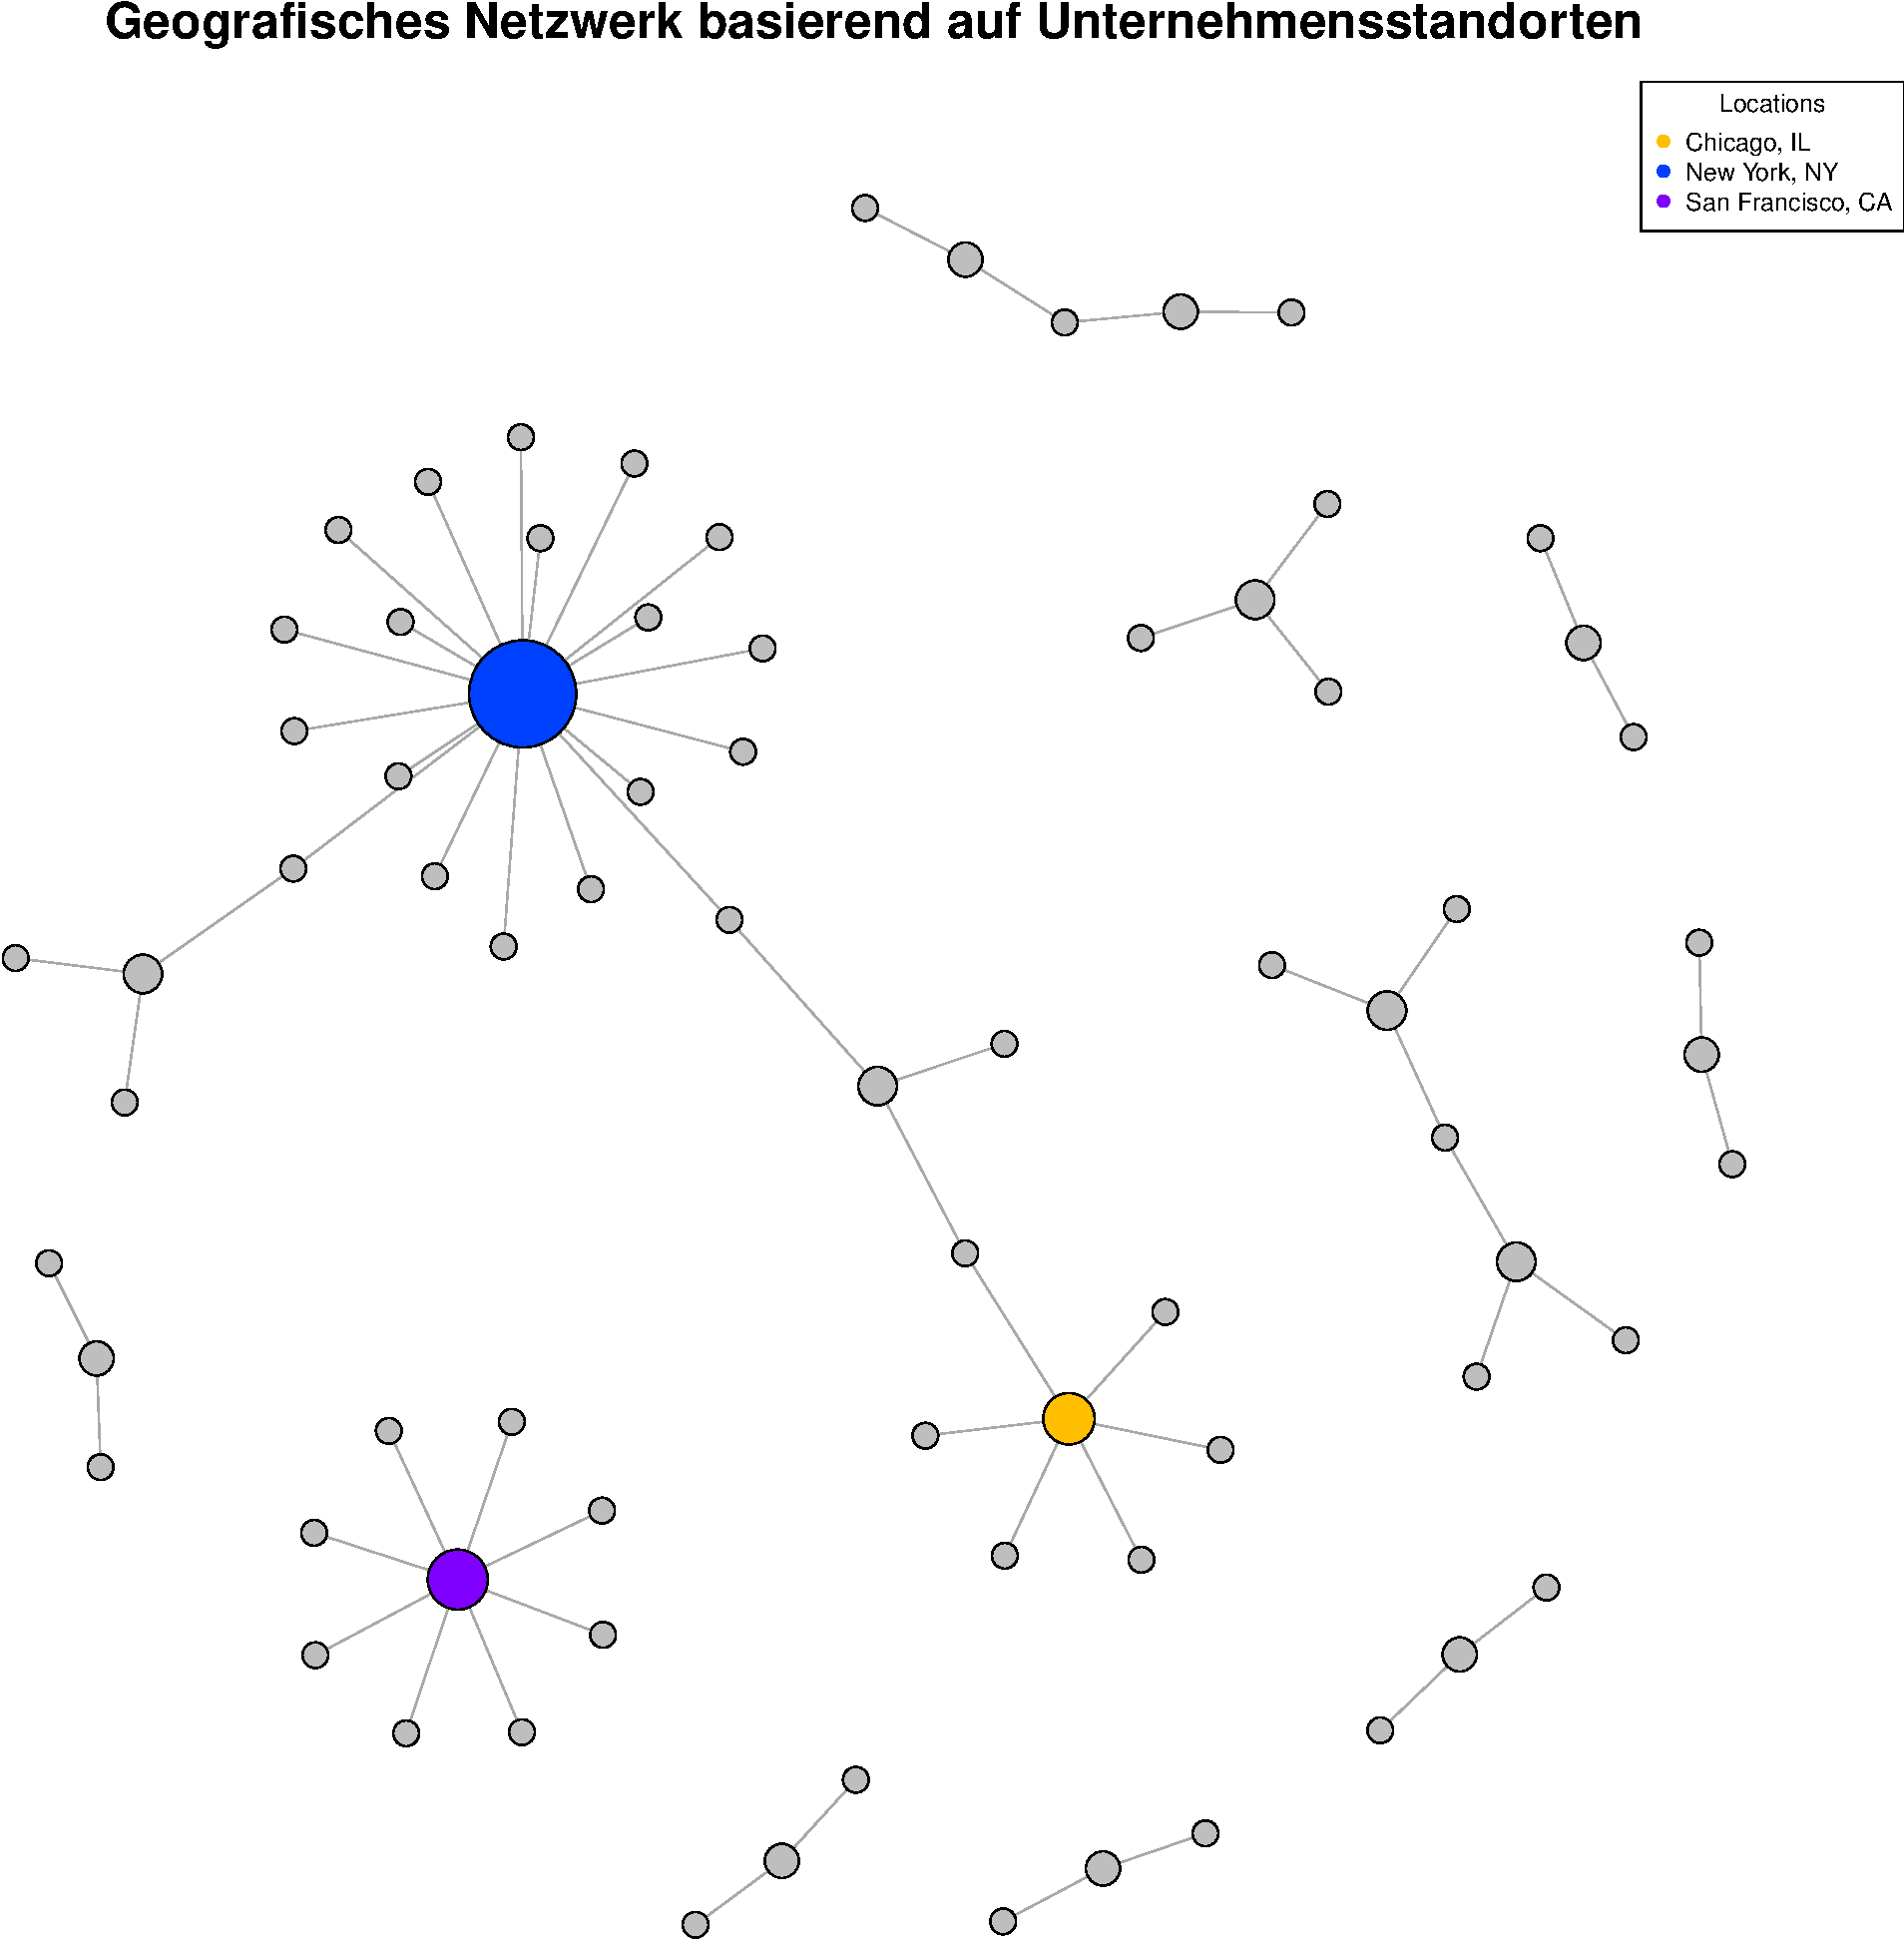
\includegraphics[keepaspectratio]{DataScience_files/figure-latex/unnamed-chunk-33-1.pdf}}

\textbf{1. Branchen mit den höchsten Durchschnittsgehältern:}

\begin{itemize}
\item
  Die Bereiche \textbf{Information Technology} und \textbf{Enterprise
  Software \& Network Solutions} gehören zu den führenden Sektoren.
  Innerhalb der Cluster 19 und 35 werden insbesondere in den genannten
  Sektoren hohe Durchschnittsgehälter erzielt.
\item
  Auch die Branchen \textbf{Consulting} und \textbf{Advertising \&
  Marketing} verzeichnen hohe Durchschnittsgehälter, insbesondere in dem
  Cluster 1.
\end{itemize}

\textbf{2. Branchen mit mittleren Gehältern:}

\begin{itemize}
\tightlist
\item
  Die mittlere Gehaltsgruppe wird insbesondere von den Clustern 19 und 5
  geprägt, wobei die Sektoren \textbf{Aerospace \& Defense} sowie
  \textbf{Insurance Carriers} eine überproportionale Bedeutung
  aufweisen. Dies lässt den Schluss zu, dass die Gehälter in diesen
  Branchen relativ stabil sind.
\end{itemize}

\textbf{3. Branchen mit niedrigeren Durchschnittsgehältern:}

\begin{itemize}
\item
  Die Branchen \textbf{Health Care Products Manufacturing} und
  \textbf{Industrial Manufacturing} sind durch ein geringeres Lohnniveau
  gekennzeichnet, insbesondere in den Clustern 8 und 12.
\item
  Die Vergütung für \textbf{IT-Services} und \textbf{Computer-Hardware
  und -Software} fällt ebenfalls eher gering aus, wobei die Cluster 1
  und 12 hier eine übergeordnete Rolle einnehmen.
\end{itemize}

\textbf{4. Clusterverteilung nach Branchen:}

\begin{itemize}
\item
  Die Analyse der Daten zeigt, dass \textbf{Cluster 19} eine
  signifikante Präsenz in hochbezahlten Branchen wie Information
  Technology und Enterprise Software \& Network Solutions aufweist. Dies
  lässt den Schluss zu, dass in diesen Bereichen ein hohes
  Gehaltspotenzial besteht.
\item
  Die Verteilung der \textbf{Cluster 1} und \textbf{Cluster 12} in den
  verschiedenen Branchen ist relativ homogen, was auf ein mittleres bis
  niedriges Gehaltsniveau in einer Vielzahl von Sektoren hindeutet.
\end{itemize}

Das vorliegende Diagramm verdeutlicht, dass bestimmte Branchen, wie
beispielsweise die Informationstechnologie sowie Enterprise Software \&
Network Solutions, über alle Cluster hinweg mit besonders hohen
Gehältern aufwarten, während andere Branchen eher auf niedrigeren
Gehaltsniveaus verbleiben.

\section{Abschließende Betrachtung mittels interaktiver
Visualisierung}\label{abschlieuxdfende-betrachtung-mittels-interaktiver-visualisierung}

Im Folgenden wird dem Leser eine interaktive Visualisierung präsentiert,
welche ihm die Möglichkeit bietet, die Ergebnisse der Wettbewerbsanalyse
eigenständig zu explorieren, bevor die Schlussfolgerungen und
Empfehlungen dargelegt werden. \(\\\)

\begin{Shaded}
\begin{Highlighting}[]
\CommentTok{\# Bereite die Daten für visNetwork vor}
\NormalTok{nodes }\OtherTok{\textless{}{-}} \FunctionTok{data.frame}\NormalTok{(}\AttributeTok{id =} \FunctionTok{V}\NormalTok{(g\_direct\_competitors)}\SpecialCharTok{$}\NormalTok{name,}
                    \AttributeTok{label =} \FunctionTok{V}\NormalTok{(g\_direct\_competitors)}\SpecialCharTok{$}\NormalTok{name,}
                    \AttributeTok{group =} \FunctionTok{membership}\NormalTok{(communities),}
                    \AttributeTok{value =}\NormalTok{ degree\_centrality,}
                    \AttributeTok{title =} \FunctionTok{paste}\NormalTok{(}\StringTok{"Degree:"}\NormalTok{, degree\_centrality, }
                                  \StringTok{"\textless{}br\textgreater{}Betweenness:"}\NormalTok{, betweenness\_centrality,}
                                  \StringTok{"\textless{}br\textgreater{}Eigenvector:"}\NormalTok{, eigenvector\_centrality,}
                                  \StringTok{"\textless{}br\textgreater{}Average Salary:"}\NormalTok{, }\FunctionTok{V}\NormalTok{(g\_direct\_competitors)}\SpecialCharTok{$}\NormalTok{salary),}
                    \AttributeTok{salary =} \FunctionTok{V}\NormalTok{(g\_direct\_competitors)}\SpecialCharTok{$}\NormalTok{salary)}

\NormalTok{edges }\OtherTok{\textless{}{-}} \FunctionTok{data.frame}\NormalTok{(}\AttributeTok{from =} \FunctionTok{as.character}\NormalTok{(edges}\SpecialCharTok{$}\NormalTok{from), }\AttributeTok{to =} \FunctionTok{as.character}\NormalTok{(edges}\SpecialCharTok{$}\NormalTok{to))}

\CommentTok{\# Erstelle eine Farbpalette basierend auf den Gehältern mit RColorBrewer}
\NormalTok{num\_colors }\OtherTok{\textless{}{-}} \DecValTok{9}
\NormalTok{color\_palette }\OtherTok{\textless{}{-}} \FunctionTok{brewer.pal}\NormalTok{(num\_colors, }\StringTok{"YlOrRd"}\NormalTok{)}
\NormalTok{nodes}\SpecialCharTok{$}\NormalTok{color }\OtherTok{\textless{}{-}}\NormalTok{ color\_palette[}\FunctionTok{cut}\NormalTok{(nodes}\SpecialCharTok{$}\NormalTok{salary, }\AttributeTok{breaks =}\NormalTok{ num\_colors, }\AttributeTok{labels =} \ConstantTok{FALSE}\NormalTok{)]}

\CommentTok{\# Erstelle die interaktive Netzwerkvisualisierung}
\NormalTok{network }\OtherTok{\textless{}{-}} \FunctionTok{visNetwork}\NormalTok{(nodes, edges) }\SpecialCharTok{\%\textgreater{}\%}
  \FunctionTok{visOptions}\NormalTok{(}\AttributeTok{highlightNearest =} \ConstantTok{TRUE}\NormalTok{, }\AttributeTok{nodesIdSelection =} \ConstantTok{TRUE}\NormalTok{) }\SpecialCharTok{\%\textgreater{}\%}
  \FunctionTok{visGroups}\NormalTok{(}\AttributeTok{groupname =} \StringTok{"1"}\NormalTok{, }\AttributeTok{color =} \StringTok{"red"}\NormalTok{) }\SpecialCharTok{\%\textgreater{}\%}
  \FunctionTok{visGroups}\NormalTok{(}\AttributeTok{groupname =} \StringTok{"2"}\NormalTok{, }\AttributeTok{color =} \StringTok{"blue"}\NormalTok{) }\SpecialCharTok{\%\textgreater{}\%}
  \FunctionTok{visGroups}\NormalTok{(}\AttributeTok{groupname =} \StringTok{"3"}\NormalTok{, }\AttributeTok{color =} \StringTok{"green"}\NormalTok{) }\SpecialCharTok{\%\textgreater{}\%}
  \FunctionTok{visGroups}\NormalTok{(}\AttributeTok{groupname =} \StringTok{"4"}\NormalTok{, }\AttributeTok{color =} \StringTok{"yellow"}\NormalTok{) }\SpecialCharTok{\%\textgreater{}\%}
  \FunctionTok{visGroups}\NormalTok{(}\AttributeTok{groupname =} \StringTok{"5"}\NormalTok{, }\AttributeTok{color =} \StringTok{"purple"}\NormalTok{) }\SpecialCharTok{\%\textgreater{}\%}
  \FunctionTok{visGroups}\NormalTok{(}\AttributeTok{groupname =} \StringTok{"6"}\NormalTok{, }\AttributeTok{color =} \StringTok{"orange"}\NormalTok{) }\SpecialCharTok{\%\textgreater{}\%}
  \FunctionTok{visGroups}\NormalTok{(}\AttributeTok{groupname =} \StringTok{"7"}\NormalTok{, }\AttributeTok{color =} \StringTok{"pink"}\NormalTok{) }\SpecialCharTok{\%\textgreater{}\%}
  \FunctionTok{visLayout}\NormalTok{(}\AttributeTok{randomSeed =} \DecValTok{123}\NormalTok{) }\SpecialCharTok{\%\textgreater{}\%}
  \FunctionTok{visLegend}\NormalTok{() }\SpecialCharTok{\%\textgreater{}\%}
  \FunctionTok{visNodes}\NormalTok{(}\AttributeTok{color =} \FunctionTok{list}\NormalTok{(}\AttributeTok{highlight =} \StringTok{"orange"}\NormalTok{))}

\CommentTok{\# Speichere die interaktive Visualisierung als HTML{-}Datei}
\FunctionTok{saveWidget}\NormalTok{(network, }\StringTok{"network.html"}\NormalTok{, }\AttributeTok{selfcontained =} \ConstantTok{TRUE}\NormalTok{)}

\CommentTok{\# Fügt ein Bild der interaktiven Netzwerkvisualisierung hinzu}
\NormalTok{knitr}\SpecialCharTok{::}\FunctionTok{include\_graphics}\NormalTok{(}\StringTok{"interaktive\_Netzwerke\_Bilder/Übersicht.png"}\NormalTok{)}
\end{Highlighting}
\end{Shaded}

\pandocbounded{\includegraphics[keepaspectratio]{interaktive_Netzwerke_Bilder/Übersicht.png}}

\begin{Shaded}
\begin{Highlighting}[]
\NormalTok{knitr}\SpecialCharTok{::}\FunctionTok{include\_graphics}\NormalTok{(}\StringTok{"interaktive\_Netzwerke\_Bilder/Deloitte.png"}\NormalTok{)}
\end{Highlighting}
\end{Shaded}

\pandocbounded{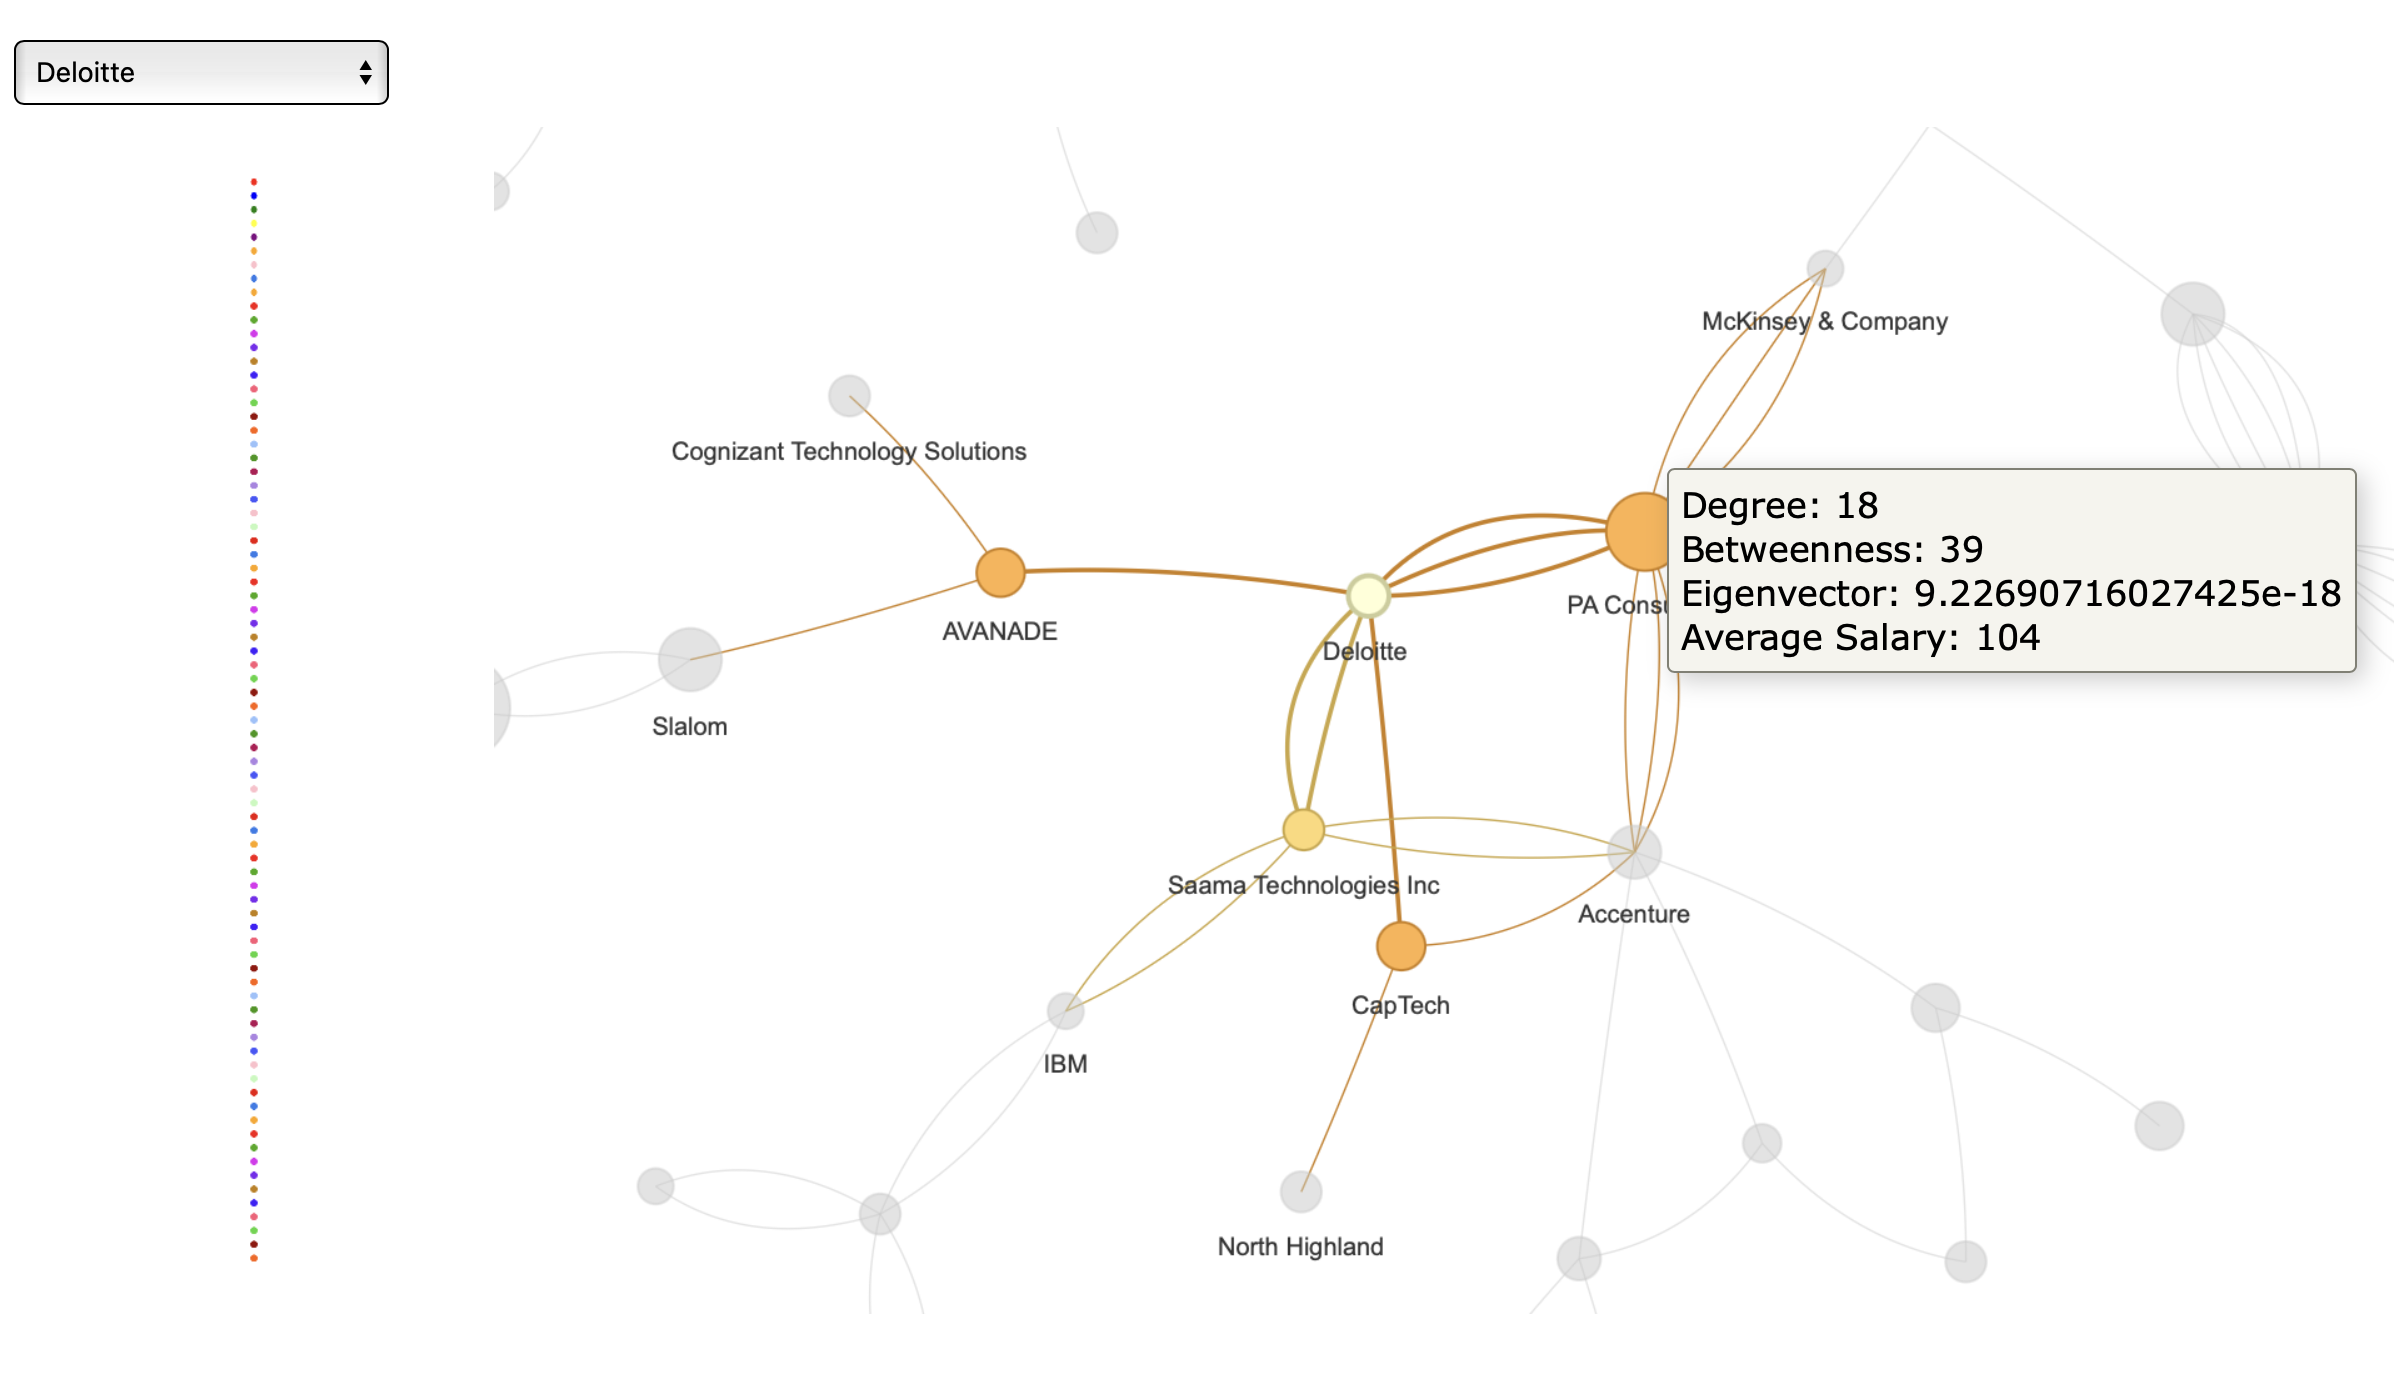
\includegraphics[keepaspectratio]{interaktive_Netzwerke_Bilder/Deloitte.png}}

Die Ausführung des Codes resultiert in der Speicherung der interaktiven
Visualisierung unter dem Namen ``network.html'' im Arbeitsverzeichnis.
Diese kann aufgerufen werden, um explorativ die Ergebnisse zu
untersuchen.

\newpage

\section{Conclusion}\label{conclusion}

Zusammenfassend zeigen die Ergebnisse dieser Arbeit überraschenderweise
wenig Zusammenhang zwischen der Wettbewerbsstruktur und den Gehältern
von Data Science-Positionen. Jedoch konnte trotzdem eine Vielzahl von
Erkenntnissen gewonnen werden, die die Rolle des Wettbewerbs im
Gehaltsgefüge von Data Science-Positionen beleuchten. \(\\\) Einerseits
zeigte die initielle Netzwerkanalyse der direkten Wettbewerber auf, dass
Unternehmen die im Mittelpunt der Wettbewerbsbeziehungen verschieder
Unternehmen stehen durchaus höhere Gehälter zahlen. Dies zeigte sich
vorallem bei erster Betrachtung, der Eindruck konnte jedoch durch
analyse der Zentralitätsmaße nicht vollends bestätigt werden.
Ausschließlich die Betweenness Centrality und Degree Centrality zeigten
einen leichten Zusammenhang mit den Gehältern, wobei die Eigenvector
Centrality keinen signifikanten Einfluss auf die Gehälter hatte. \(\\\)
Die Clusteranalyse ergab eine signifikante Varianz der Gehälter zwischen
den Clustern. Die Cluster 1, 8, 35, 5, 15, 19, 12 erwiesen sich als die
größten Cluster, wobei Cluster 19 die höchsten Durchschnittsgehälter
aufwies. Dabei entpuppten sich die Branchen Informationstechnologie und
Enterprise Software \& Network Solutions in den zentralen Clustern als
besonders lukrativ, während andere Branchen eher niedrigere Gehälter
aufwiesen. \(\\\) Insgesamt lässt sich festhalten, dass das
Wettbewerbsumfeld und die Netzwerkposition zwar ein entscheidender
Faktor für die Gehaltsstruktur im Data Science-Bereich ist, es jedoch
sehr wahrscheinlich ist, dass andere Einflussfaktoren eine ähnliche oder
sogar größere Rolle spielen könnten.

Die in dieser Arbeit gewonnenen Erkenntnisse bieten Ansatzpunkte für
weiterführende Untersuchungen. Eine naheliegende Erweiterung wäre die
Einbeziehung zusätzlicher Einflussfaktoren wie Unternehmensgröße,
Branche oder Standort, um ein noch differenzierteres Bild des
Zusammenhangs zwischen Wettbewerbsstruktur und Lohnniveau zu erhalten.
Ein erster Schritt in diese Richtung wurde im Rahmen dieser Arbeit
bereits unternommen (siehe Anhang). \(\\\) Eine weitere Möglichkeit wäre
die Durchführung einer Regressionsanalyse, um den Einfluss der
Wettbewerbsstruktur auf die Gehälter quantitativ genauer zu erfassen.
Dies könnte zu einem besseren Verständnis der Auswirkungen verschiedener
Wettbewerbsfaktoren auf die Vergütung im Bereich Data Science beitragen.
\(\\\) Darüber hinaus wäre es denkbar, aus den Ergebnissen dieser Arbeit
konkrete Handlungsempfehlungen für Unternehmen oder Arbeitnehmer
abzuleiten, um ihnen eine Orientierung im Wettbewerb um Talente im
Bereich Data Science zu geben. Dies würde jedoch den Rahmen dieser
Arbeit sprengen und könnte als eigenständiges Forschungsprojekt verfolgt
werden.

\newpage

\section{Anhang}\label{anhang}

\subsection{Geografische Betrachtung}\label{geografische-betrachtung}

Da bei der Betrachtung der Wettbewerbsstruktur die geografische Nähe von
Unternehmen auch eine Rolle spielen kann, soll zunächst ein Netzwerk
erstellt werden, das auf der geografischen Nähe von Unternehmen basiert.
Diese annahme beruht darauf, dass Unternehmen in derselben Region
wahrscheinlich ähnliche Gehälter anbieten. Dies soll Überprüft werden um
diese Arbeit um eine weiter Dimension zu erweitern.

\subsubsection{Erstellung eines Geografischen
Netzwerkes}\label{erstellung-eines-geografischen-netzwerkes}

Die Gewichtung erfolgt linear, wobei jeder Standort eine Grundgröße von
3 hat, und für jedes Unternehmen an diesem Standort wird die Größe um
0.5 erhöht. Ab einer Größe von 4.5 wird die Farbe des Standorts
geändert, um die Standorte mit mehreren Unternehmen hervorzuheben.
\(\\\)

\begin{Shaded}
\begin{Highlighting}[]
\CommentTok{\# Aus Gründen der Sichtbarkeit, werden bloß Locations mit mehr als einem}
\CommentTok{\# Unternehmen dargestellt.}

\CommentTok{\# Extract relevant columns for geographic visualization}
\NormalTok{edges\_geo }\OtherTok{\textless{}{-}}\NormalTok{ data }\SpecialCharTok{\%\textgreater{}\%}
  \FunctionTok{select}\NormalTok{(}\AttributeTok{Company =} \StringTok{\textasciigrave{}}\AttributeTok{Company Name}\StringTok{\textasciigrave{}}\NormalTok{, }\AttributeTok{Location =} \StringTok{\textasciigrave{}}\AttributeTok{Location}\StringTok{\textasciigrave{}}\NormalTok{) }\SpecialCharTok{\%\textgreater{}\%}
  \FunctionTok{distinct}\NormalTok{()}

\CommentTok{\# Calculate the number of companies per location and filter for locations}
\CommentTok{\# with more than one company}
\NormalTok{location\_counts }\OtherTok{\textless{}{-}}\NormalTok{ edges\_geo }\SpecialCharTok{\%\textgreater{}\%}
  \FunctionTok{group\_by}\NormalTok{(Location) }\SpecialCharTok{\%\textgreater{}\%}
  \FunctionTok{summarise}\NormalTok{(}\AttributeTok{Company\_Count =} \FunctionTok{n}\NormalTok{()) }\SpecialCharTok{\%\textgreater{}\%}
  \FunctionTok{filter}\NormalTok{(Company\_Count }\SpecialCharTok{\textgreater{}} \DecValTok{1}\NormalTok{)  }\CommentTok{\# Keep only locations with more than one company}

\CommentTok{\# Filter edges to include only connections for locations with more than}
\CommentTok{\# one company}
\NormalTok{filtered\_edges }\OtherTok{\textless{}{-}}\NormalTok{ edges\_geo }\SpecialCharTok{\%\textgreater{}\%}
  \FunctionTok{filter}\NormalTok{(Location }\SpecialCharTok{\%in\%}\NormalTok{ location\_counts}\SpecialCharTok{$}\NormalTok{Location)}

\CommentTok{\# Create an igraph object for geographic visualization}
\NormalTok{network\_geo }\OtherTok{\textless{}{-}} \FunctionTok{graph\_from\_data\_frame}\NormalTok{(filtered\_edges, }\AttributeTok{directed =} \ConstantTok{FALSE}\NormalTok{)}

\CommentTok{\# Set vertex colors based on whether the node is a company or a location}
\NormalTok{company\_colors }\OtherTok{\textless{}{-}} \StringTok{"blue"}
\NormalTok{location\_colors }\OtherTok{\textless{}{-}} \FunctionTok{rainbow}\NormalTok{(}\FunctionTok{nrow}\NormalTok{(location\_counts))}

\CommentTok{\# Set vertex size based on the number of companies at each location}
\NormalTok{vertex\_sizes }\OtherTok{\textless{}{-}} \FunctionTok{ifelse}\NormalTok{(}\FunctionTok{V}\NormalTok{(network\_geo)}\SpecialCharTok{$}\NormalTok{name }\SpecialCharTok{\%in\%}\NormalTok{ location\_counts}\SpecialCharTok{$}\NormalTok{Location,}
                       \DecValTok{3} \SpecialCharTok{+}\NormalTok{ location\_counts}\SpecialCharTok{$}\NormalTok{Company\_Count[}
                         \FunctionTok{match}\NormalTok{(}\FunctionTok{V}\NormalTok{(network\_geo)}\SpecialCharTok{$}\NormalTok{name, location\_counts}\SpecialCharTok{$}\NormalTok{Location)}
\NormalTok{                       ] }\SpecialCharTok{*} \FloatTok{0.5}\NormalTok{,  }\CommentTok{\# Linear scaling factor with minimum size 3}
                       \DecValTok{3}\NormalTok{) }\CommentTok{\# Default size for companies}

\CommentTok{\# Assign colors and sizes to vertices}
\FunctionTok{V}\NormalTok{(network\_geo)}\SpecialCharTok{$}\NormalTok{size }\OtherTok{\textless{}{-}}\NormalTok{ vertex\_sizes}
\FunctionTok{V}\NormalTok{(network\_geo)}\SpecialCharTok{$}\NormalTok{color }\OtherTok{\textless{}{-}} \FunctionTok{ifelse}\NormalTok{(}\FunctionTok{V}\NormalTok{(network\_geo)}\SpecialCharTok{$}\NormalTok{name }\SpecialCharTok{\%in\%}\NormalTok{ location\_counts}\SpecialCharTok{$}\NormalTok{Location }\SpecialCharTok{\&}
\NormalTok{                               vertex\_sizes }\SpecialCharTok{\textgreater{}} \FloatTok{4.5}\NormalTok{,}
\NormalTok{                               location\_colors[}
                                 \FunctionTok{match}\NormalTok{(}\FunctionTok{V}\NormalTok{(network\_geo)}\SpecialCharTok{$}\NormalTok{name, location\_counts}\SpecialCharTok{$}\NormalTok{Location)}
\NormalTok{                               ],}
                               \StringTok{"grey"}\NormalTok{)}

\CommentTok{\# Plot the network}
\FunctionTok{plot}\NormalTok{(network\_geo,}
     \AttributeTok{vertex.label =} \ConstantTok{NA}\NormalTok{,  }\CommentTok{\# Remove labels from the plot}
     \AttributeTok{vertex.size =} \FunctionTok{V}\NormalTok{(network\_geo)}\SpecialCharTok{$}\NormalTok{size,}
     \AttributeTok{vertex.color =} \FunctionTok{V}\NormalTok{(network\_geo)}\SpecialCharTok{$}\NormalTok{color,}
     \AttributeTok{edge.arrow.size =} \FloatTok{0.3}\NormalTok{,}
     \AttributeTok{layout =}\NormalTok{ layout\_with\_fr,}
\NormalTok{)}

\CommentTok{\# Add legend for locations with size \textgreater{} 4.5}
\NormalTok{location\_indices }\OtherTok{\textless{}{-}} \FunctionTok{match}\NormalTok{(location\_counts}\SpecialCharTok{$}\NormalTok{Location, }\FunctionTok{V}\NormalTok{(network\_geo)}\SpecialCharTok{$}\NormalTok{name)}
\NormalTok{large\_locations }\OtherTok{\textless{}{-}}\NormalTok{ location\_counts}\SpecialCharTok{$}\NormalTok{Location[vertex\_sizes[location\_indices] }\SpecialCharTok{\textgreater{}} \FloatTok{4.5}\NormalTok{]}

\NormalTok{large\_location\_colors }\OtherTok{\textless{}{-}}\NormalTok{ location\_colors[}
  \FunctionTok{match}\NormalTok{(large\_locations, location\_counts}\SpecialCharTok{$}\NormalTok{Location)}
\NormalTok{]}
\FunctionTok{legend}\NormalTok{(}\StringTok{"topright"}\NormalTok{,}
       \AttributeTok{legend =}\NormalTok{ large\_locations,}
       \AttributeTok{col =}\NormalTok{ large\_location\_colors,}
       \AttributeTok{pch =} \DecValTok{19}\NormalTok{,}
       \AttributeTok{title =} \StringTok{"Locations"}\NormalTok{)}

\FunctionTok{title}\NormalTok{(}\AttributeTok{main =} \StringTok{"Geografisches Netzwerk basierend auf Unternehmensstandorten"}\NormalTok{, }\AttributeTok{cex.main =} \DecValTok{2}\NormalTok{)}
\end{Highlighting}
\end{Shaded}

\pandocbounded{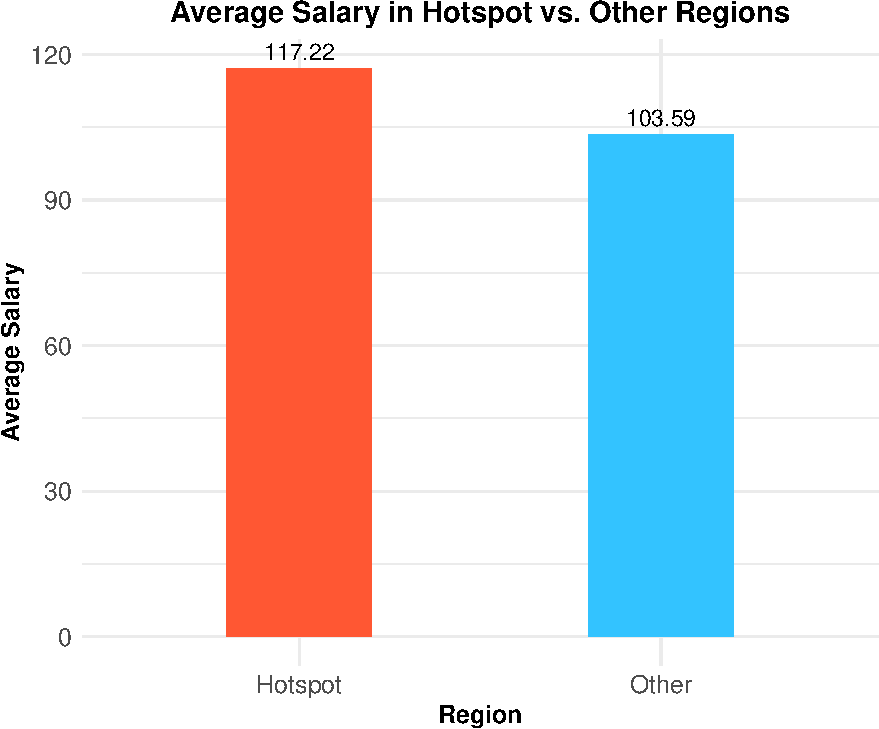
\includegraphics[keepaspectratio]{DataScience_files/figure-latex/unnamed-chunk-35-1.pdf}}

Wie zu erwarten war, sind die meisten Unternehmen in Ballungszentren wie
New York, Chicago und San Francisco angesiedelt.

\subsubsection{Vergleich der Gehälter zwischen den Hotspot- und den
anderen
Regionen}\label{vergleich-der-gehuxe4lter-zwischen-den-hotspot--und-den-anderen-regionen}

\begin{Shaded}
\begin{Highlighting}[]
\CommentTok{\# Ausgabe der farbigen Standorte}
\FunctionTok{print}\NormalTok{(large\_locations)}
\end{Highlighting}
\end{Shaded}

\begin{verbatim}
## [1] "Chicago, IL"       "New York, NY"      "San Francisco, CA"
\end{verbatim}

\begin{Shaded}
\begin{Highlighting}[]
\CommentTok{\# Filterung der Daten für die Hotspot{-}Regionen}
\NormalTok{data\_hotspots }\OtherTok{\textless{}{-}}\NormalTok{ data }\SpecialCharTok{\%\textgreater{}\%}
  \FunctionTok{filter}\NormalTok{(}\StringTok{\textasciigrave{}}\AttributeTok{Location}\StringTok{\textasciigrave{}} \SpecialCharTok{\%in\%}\NormalTok{ large\_locations)}

\CommentTok{\# Filterung der Daten für die anderen Regionen}
\NormalTok{data\_other }\OtherTok{\textless{}{-}}\NormalTok{ data }\SpecialCharTok{\%\textgreater{}\%}
  \FunctionTok{filter}\NormalTok{(}\SpecialCharTok{!}\StringTok{\textasciigrave{}}\AttributeTok{Location}\StringTok{\textasciigrave{}} \SpecialCharTok{\%in\%}\NormalTok{ large\_locations)}

\CommentTok{\# Durchschnittsgehalt in den Hotspot{-}Regionen}
\NormalTok{avg\_salary\_hotspots }\OtherTok{\textless{}{-}} \FunctionTok{mean}\NormalTok{(data\_hotspots}\SpecialCharTok{$}\StringTok{\textasciigrave{}}\AttributeTok{Salary Estimate}\StringTok{\textasciigrave{}}\NormalTok{, }\AttributeTok{na.rm =} \ConstantTok{TRUE}\NormalTok{)}

\CommentTok{\# Durchschnittsgehalt in den anderen Regionen}
\NormalTok{avg\_salary\_other }\OtherTok{\textless{}{-}} \FunctionTok{mean}\NormalTok{(data\_other}\SpecialCharTok{$}\StringTok{\textasciigrave{}}\AttributeTok{Salary Estimate}\StringTok{\textasciigrave{}}\NormalTok{, }\AttributeTok{na.rm =} \ConstantTok{TRUE}\NormalTok{)}

\CommentTok{\# Erstellung eines Balkendiagramms}
\FunctionTok{ggplot}\NormalTok{(}\AttributeTok{data =} \FunctionTok{data.frame}\NormalTok{(}\AttributeTok{Region =} \FunctionTok{c}\NormalTok{(}\StringTok{"Hotspot"}\NormalTok{, }\StringTok{"Other"}\NormalTok{),}
                         \AttributeTok{Average\_Salary =} \FunctionTok{c}\NormalTok{(avg\_salary\_hotspots,}
\NormalTok{                                            avg\_salary\_other)),}
       \FunctionTok{aes}\NormalTok{(}\AttributeTok{x =}\NormalTok{ Region, }\AttributeTok{y =}\NormalTok{ Average\_Salary, }\AttributeTok{fill =}\NormalTok{ Region)) }\SpecialCharTok{+}
  \FunctionTok{geom\_bar}\NormalTok{(}\AttributeTok{stat =} \StringTok{"identity"}\NormalTok{, }\AttributeTok{width =} \FloatTok{0.4}\NormalTok{) }\SpecialCharTok{+}
  \FunctionTok{scale\_fill\_manual}\NormalTok{(}\AttributeTok{values =} \FunctionTok{c}\NormalTok{(}\StringTok{"Hotspot"} \OtherTok{=} \StringTok{"\#FF5733"}\NormalTok{, }\StringTok{"Other"} \OtherTok{=} \StringTok{"\#33C3FF"}\NormalTok{)) }\SpecialCharTok{+}
  \FunctionTok{labs}\NormalTok{(}\AttributeTok{title =} \StringTok{"Average Salary in Hotspot vs. Other Regions"}\NormalTok{,}
       \AttributeTok{x =} \StringTok{"Region"}\NormalTok{,}
       \AttributeTok{y =} \StringTok{"Average Salary"}\NormalTok{) }\SpecialCharTok{+}
  \FunctionTok{theme\_minimal}\NormalTok{() }\SpecialCharTok{+}
  \FunctionTok{theme}\NormalTok{(}
    \AttributeTok{plot.title =} \FunctionTok{element\_text}\NormalTok{(}\AttributeTok{hjust =} \FloatTok{0.5}\NormalTok{, }\AttributeTok{size =} \DecValTok{14}\NormalTok{, }\AttributeTok{face =} \StringTok{"bold"}\NormalTok{),}
    \AttributeTok{axis.title.x =} \FunctionTok{element\_text}\NormalTok{(}\AttributeTok{size =} \DecValTok{12}\NormalTok{, }\AttributeTok{face =} \StringTok{"bold"}\NormalTok{),}
    \AttributeTok{axis.title.y =} \FunctionTok{element\_text}\NormalTok{(}\AttributeTok{size =} \DecValTok{12}\NormalTok{, }\AttributeTok{face =} \StringTok{"bold"}\NormalTok{),}
    \AttributeTok{axis.text.x =} \FunctionTok{element\_text}\NormalTok{(}\AttributeTok{size =} \DecValTok{12}\NormalTok{),}
    \AttributeTok{axis.text.y =} \FunctionTok{element\_text}\NormalTok{(}\AttributeTok{size =} \DecValTok{12}\NormalTok{),}
    \AttributeTok{legend.position =} \StringTok{"none"}
\NormalTok{  ) }\SpecialCharTok{+}
  \FunctionTok{geom\_text}\NormalTok{(}\FunctionTok{aes}\NormalTok{(}\AttributeTok{label =} \FunctionTok{round}\NormalTok{(Average\_Salary, }\DecValTok{2}\NormalTok{)), }\AttributeTok{vjust =} \SpecialCharTok{{-}}\FloatTok{0.5}\NormalTok{, }\AttributeTok{size =} \DecValTok{4}\NormalTok{)}
\end{Highlighting}
\end{Shaded}

\pandocbounded{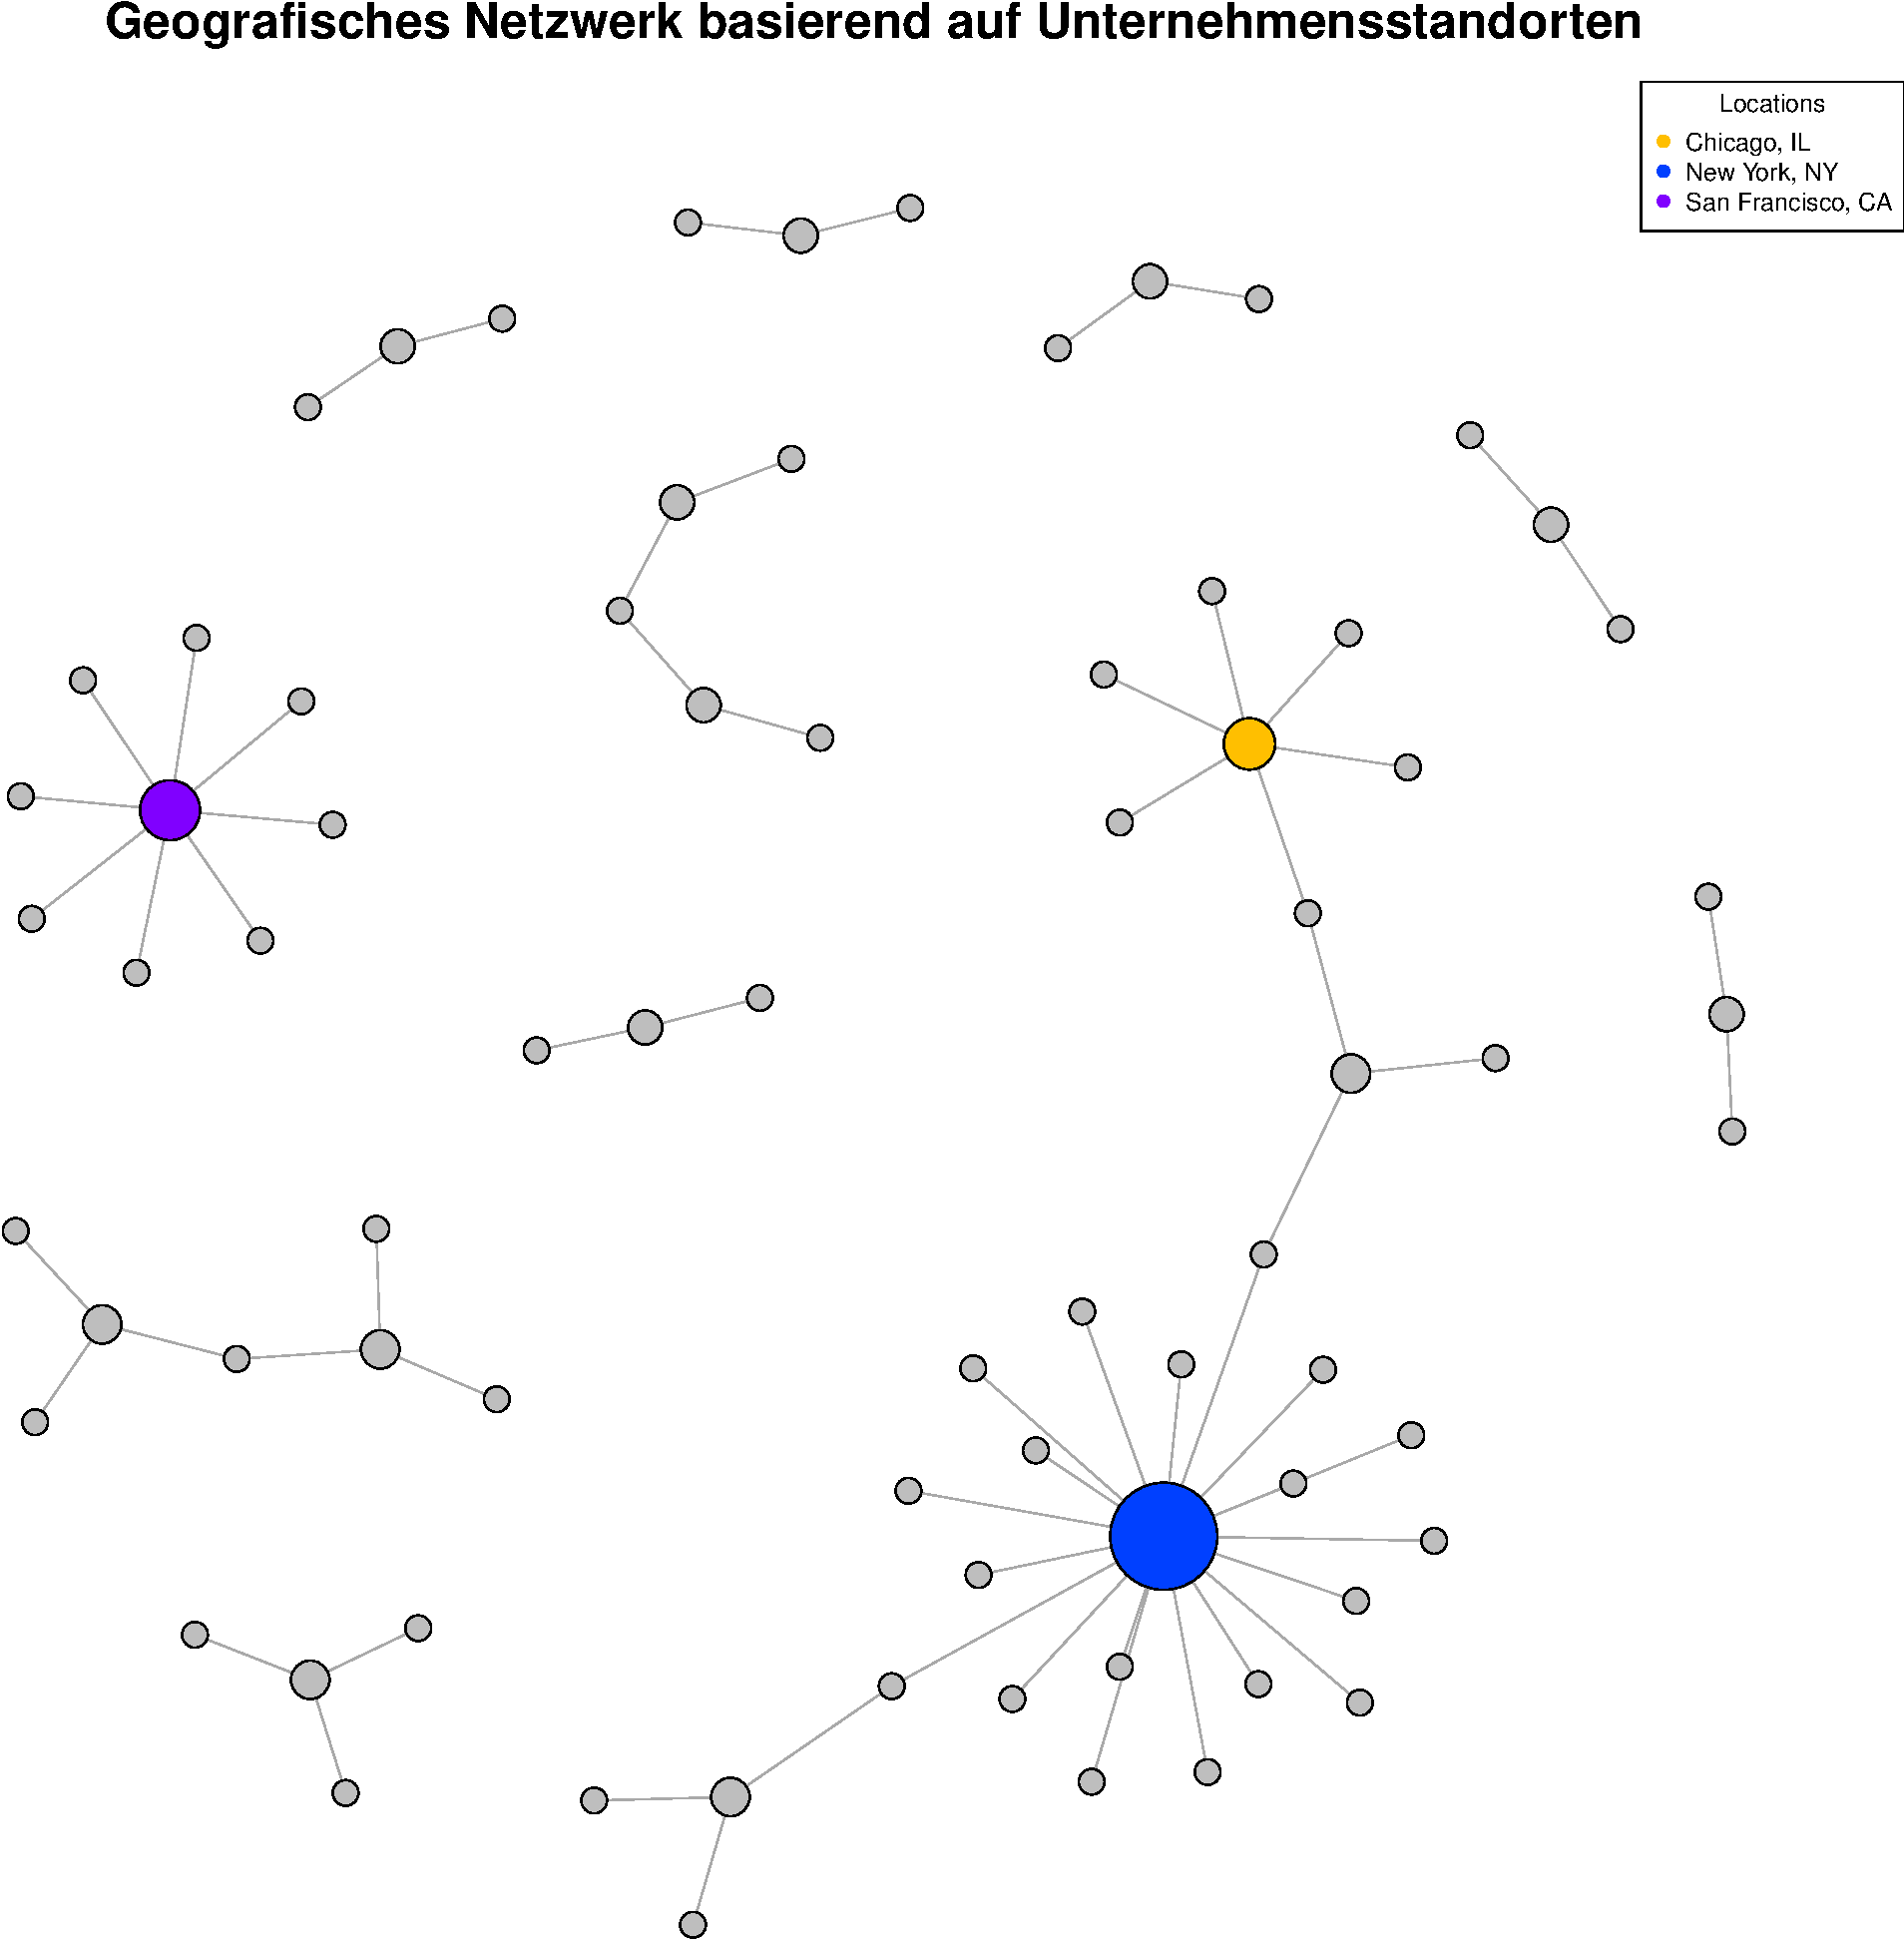
\includegraphics[keepaspectratio]{DataScience_files/figure-latex/unnamed-chunk-36-1.pdf}}

\begin{Shaded}
\begin{Highlighting}[]
\CommentTok{\# Berechnung der Gehaltsunterschiede}
\NormalTok{salary\_diff }\OtherTok{\textless{}{-}}\NormalTok{ avg\_salary\_hotspots }\SpecialCharTok{{-}}\NormalTok{ avg\_salary\_other}

\CommentTok{\# Ausgabe der Gehaltsunterschiede}
\FunctionTok{print}\NormalTok{(}\FunctionTok{paste}\NormalTok{(}\StringTok{"Durchschnittsgehalt in Hotspot{-}Regionen:"}\NormalTok{, avg\_salary\_hotspots))}
\end{Highlighting}
\end{Shaded}

\begin{verbatim}
## [1] "Durchschnittsgehalt in Hotspot-Regionen: 117.223880597015"
\end{verbatim}

\begin{Shaded}
\begin{Highlighting}[]
\FunctionTok{print}\NormalTok{(}\FunctionTok{paste}\NormalTok{(}\StringTok{"Durchschnittsgehalt in anderen Regionen:"}\NormalTok{, avg\_salary\_other))}
\end{Highlighting}
\end{Shaded}

\begin{verbatim}
## [1] "Durchschnittsgehalt in anderen Regionen: 103.59"
\end{verbatim}

\begin{Shaded}
\begin{Highlighting}[]
\FunctionTok{print}\NormalTok{(}\FunctionTok{paste}\NormalTok{(}\StringTok{"Durchschnittlicher Gehaltsunterschied:"}\NormalTok{, salary\_diff))}
\end{Highlighting}
\end{Shaded}

\begin{verbatim}
## [1] "Durchschnittlicher Gehaltsunterschied: 13.6338805970149"
\end{verbatim}

Das Ergebniss zeigt, dass entsprechend der vorher getroffenen Annahme,
die Gehälter in den Hotspot-Regionen im Durchschnitt höher sind als in
anderen Regionen. Dies impliziert eine Korrelation zwischen
geografischer Nähe und Gehaltsniveau. Eine mögliche Erlärung hierfür
könnte die höhere Lebenshaltungskosten in Ballungszentren sein, die
höhere Gehälter erforderlich machen.

\newpage

\section{Literaturverzeichnis}\label{literaturverzeichnis}

Davenport, Thomas H.; Patil, D. J. 2012. »Data Scientist: The Sexiest
Job of the 21st Century«, in Harvard Business Review vom 1. Oktober
2012.
\url{https://hbr.org/2012/10/data-scientist-the-sexiest-job-of-the-21st-century}
(Zugriff vom 30.10.2024).

Google Trends,
\url{https://trends.google.com/trends/explore?date=all&q=\%22data\%20science\%22,\%22data\%20scientist\%22}
(Zugriff vom 30.10.2024).

Mahanti, Rupa 2021. »Data and Its Governance«, in Data Governance and
Data Management: Contextualizing Data Governance Drivers, Technologies,
and Tools, hrsg. v. Mahanti, Rupa, S. 5--82. Singapore: Springer.

Rydning, David Reinsel--John Gantz--John 2018. »The Digitization of the
World From Edge to Core«.

Stockinger, Kurt; Stadelmann, Thilo; Ruckstuhl, Andreas 2016. »Data
Scientist als Beruf«, in Big Data: Grundlagen, Systeme und
Nutzungspotenziale, hrsg. v. Fasel, Daniel; Meier, Andreas, S. 59-61.
Wiesbaden: Springer Fachmedien.

»The world's most valuable resource is no longer oil, but data«, in The
Economist vom 6. Mai 2017.
\url{https://www.economist.com/leaders/2017/05/06/the-worlds-most-valuable-resource-is-no-longer-oil-but-data}
(Zugriff vom 11.13.2024).

\includepdf[pages=-]{KI_Selbstständigkeit.pdf}

\end{document}
